\documentclass[twoside]{book}

% Packages required by doxygen
\usepackage{fixltx2e}
\usepackage{calc}
\usepackage{doxygen}
\usepackage[export]{adjustbox} % also loads graphicx
\usepackage{graphicx}
\usepackage[utf8]{inputenc}
\usepackage{makeidx}
\usepackage{multicol}
\usepackage{multirow}
\PassOptionsToPackage{warn}{textcomp}
\usepackage{textcomp}
\usepackage[nointegrals]{wasysym}
\usepackage[table]{xcolor}

% Font selection
\usepackage[T1]{fontenc}
\usepackage[scaled=.90]{helvet}
\usepackage{courier}
\usepackage{amssymb}
\usepackage{sectsty}
\renewcommand{\familydefault}{\sfdefault}
\allsectionsfont{%
  \fontseries{bc}\selectfont%
  \color{darkgray}%
}
\renewcommand{\DoxyLabelFont}{%
  \fontseries{bc}\selectfont%
  \color{darkgray}%
}
\newcommand{\+}{\discretionary{\mbox{\scriptsize$\hookleftarrow$}}{}{}}

% Page & text layout
\usepackage{geometry}
\geometry{%
  a4paper,%
  top=2.5cm,%
  bottom=2.5cm,%
  left=2.5cm,%
  right=2.5cm%
}
\tolerance=750
\hfuzz=15pt
\hbadness=750
\setlength{\emergencystretch}{15pt}
\setlength{\parindent}{0cm}
\setlength{\parskip}{3ex plus 2ex minus 2ex}
\makeatletter
\renewcommand{\paragraph}{%
  \@startsection{paragraph}{4}{0ex}{-1.0ex}{1.0ex}{%
    \normalfont\normalsize\bfseries\SS@parafont%
  }%
}
\renewcommand{\subparagraph}{%
  \@startsection{subparagraph}{5}{0ex}{-1.0ex}{1.0ex}{%
    \normalfont\normalsize\bfseries\SS@subparafont%
  }%
}
\makeatother

% Headers & footers
\usepackage{fancyhdr}
\pagestyle{fancyplain}
\fancyhead[LE]{\fancyplain{}{\bfseries\thepage}}
\fancyhead[CE]{\fancyplain{}{}}
\fancyhead[RE]{\fancyplain{}{\bfseries\leftmark}}
\fancyhead[LO]{\fancyplain{}{\bfseries\rightmark}}
\fancyhead[CO]{\fancyplain{}{}}
\fancyhead[RO]{\fancyplain{}{\bfseries\thepage}}
\fancyfoot[LE]{\fancyplain{}{}}
\fancyfoot[CE]{\fancyplain{}{}}
\fancyfoot[RE]{\fancyplain{}{\bfseries\scriptsize Generated by Doxygen }}
\fancyfoot[LO]{\fancyplain{}{\bfseries\scriptsize Generated by Doxygen }}
\fancyfoot[CO]{\fancyplain{}{}}
\fancyfoot[RO]{\fancyplain{}{}}
\renewcommand{\footrulewidth}{0.4pt}
\renewcommand{\chaptermark}[1]{%
  \markboth{#1}{}%
}
\renewcommand{\sectionmark}[1]{%
  \markright{\thesection\ #1}%
}

% Indices & bibliography
\usepackage{natbib}
\usepackage[titles]{tocloft}
\setcounter{tocdepth}{3}
\setcounter{secnumdepth}{5}
\makeindex

% Custom commands
\newcommand{\clearemptydoublepage}{%
  \newpage{\pagestyle{empty}\cleardoublepage}%
}

\usepackage{caption}
\captionsetup{labelsep=space,justification=centering,font={bf},singlelinecheck=off,skip=4pt,position=top}

%===== C O N T E N T S =====

\begin{document}

% Titlepage & ToC
\pagenumbering{roman}
\begin{titlepage}
\vspace*{7cm}
\begin{center}%
{\Large P\+DF Search Engine }\\
\vspace*{1cm}
{\large Generated by Doxygen 1.8.11}\\
\end{center}
\end{titlepage}
\clearemptydoublepage
\tableofcontents
\clearemptydoublepage
\pagenumbering{arabic}

%--- Begin generated contents ---
\chapter{Module Index}
\section{Modules}
Here is a list of all modules\+:\begin{DoxyCompactList}
\item \contentsline{section}{Indexing}{\pageref{group___indexing}}{}
\item \contentsline{section}{Debugging}{\pageref{group___debugging}}{}
\item \contentsline{section}{Stemming}{\pageref{group___stemming}}{}
\item \contentsline{section}{Mathematics}{\pageref{group___mathematics}}{}
\item \contentsline{section}{String\+Operations}{\pageref{group___string_operations}}{}
\item \contentsline{section}{Utilities}{\pageref{group___utilities}}{}
\end{DoxyCompactList}

\chapter{Namespace Index}
\section{Namespace List}
Here is a list of all documented namespaces with brief descriptions\+:\begin{DoxyCompactList}
\item\contentsline{section}{{\bf stemming} \\*Namespace for stemming classes }{\pageref{namespacestemming}}{}
\item\contentsline{section}{{\bf string\+\_\+util} }{\pageref{namespacestring__util}}{}
\end{DoxyCompactList}

\chapter{Hierarchical Index}
\section{Class Hierarchy}
This inheritance list is sorted roughly, but not completely, alphabetically\+:\begin{DoxyCompactList}
\item \contentsline{section}{backup\+\_\+variable$<$ T $>$}{\pageref{classbackup__variable}}{}
\item binary\+\_\+function\begin{DoxyCompactList}
\item \contentsline{section}{double\+\_\+less}{\pageref{classdouble__less}}{}
\item \contentsline{section}{string\+\_\+util\+:\+:equal\+\_\+basic\+\_\+string\+\_\+i\+\_\+compare$<$ T $>$}{\pageref{classstring__util_1_1equal__basic__string__i__compare}}{}
\item \contentsline{section}{string\+\_\+util\+:\+:equal\+\_\+string\+\_\+compare$<$ T $>$}{\pageref{classstring__util_1_1equal__string__compare}}{}
\item \contentsline{section}{string\+\_\+util\+:\+:equal\+\_\+string\+\_\+i\+\_\+compare$<$ T $>$}{\pageref{classstring__util_1_1equal__string__i__compare}}{}
\item \contentsline{section}{string\+\_\+util\+:\+:less\+\_\+basic\+\_\+string\+\_\+compare$<$ T $>$}{\pageref{classstring__util_1_1less__basic__string__compare}}{}
\item \contentsline{section}{string\+\_\+util\+:\+:less\+\_\+string\+\_\+compare$<$ T $>$}{\pageref{classstring__util_1_1less__string__compare}}{}
\item \contentsline{section}{string\+\_\+util\+:\+:less\+\_\+string\+\_\+i\+\_\+compare$<$ T $>$}{\pageref{classstring__util_1_1less__string__i__compare}}{}
\item \contentsline{section}{string\+\_\+util\+:\+:less\+\_\+string\+\_\+n\+\_\+compare$<$ T $>$}{\pageref{classstring__util_1_1less__string__n__compare}}{}
\item \contentsline{section}{string\+\_\+util\+:\+:less\+\_\+string\+\_\+natural\+\_\+order\+\_\+i\+\_\+compare$<$ T $>$}{\pageref{classstring__util_1_1less__string__natural__order__i__compare}}{}
\item \contentsline{section}{string\+\_\+util\+:\+:less\+\_\+string\+\_\+ni\+\_\+compare$<$ T $>$}{\pageref{classstring__util_1_1less__string__ni__compare}}{}
\end{DoxyCompactList}
\item \contentsline{section}{bookmark}{\pageref{structbookmark}}{}
\item \contentsline{section}{document}{\pageref{structdocument}}{}
\item \contentsline{section}{Document\+Parser}{\pageref{class_document_parser}}{}
\item \contentsline{section}{index\+\_\+node}{\pageref{structindex__node}}{}
\item \contentsline{section}{indexextractor}{\pageref{classindexextractor}}{}
\item \contentsline{section}{Index\+Handler}{\pageref{class_index_handler}}{}
\item \contentsline{section}{Index\+Interface}{\pageref{class_index_interface}}{}
\begin{DoxyCompactList}
\item \contentsline{section}{A\+V\+L\+Tree\+Index}{\pageref{class_a_v_l_tree_index}}{}
\item \contentsline{section}{hashy}{\pageref{classhashy}}{}
\end{DoxyCompactList}
\item \contentsline{section}{item}{\pageref{structitem}}{}
\item \contentsline{section}{stemming\+:\+:no\+\_\+op\+\_\+stem$<$ string\+\_\+typeT $>$}{\pageref{classstemming_1_1no__op__stem}}{}
\item pair\begin{DoxyCompactList}
\item \contentsline{section}{comparable\+\_\+first\+\_\+pair$<$ T1, T2 $>$}{\pageref{classcomparable__first__pair}}{}
\end{DoxyCompactList}
\item \contentsline{section}{Query\+Engine}{\pageref{class_query_engine}}{}
\item \contentsline{section}{raw\+Output\+Extractor}{\pageref{classraw_output_extractor}}{}
\item \contentsline{section}{Search\+Engine}{\pageref{class_search_engine}}{}
\item \contentsline{section}{stemming\+:\+:stem$<$ string\+\_\+typeT $>$}{\pageref{classstemming_1_1stem}}{}
\begin{DoxyCompactList}
\item \contentsline{section}{stemming\+:\+:english\+\_\+stem$<$ string\+\_\+typeT $>$}{\pageref{classstemming_1_1english__stem}}{}
\end{DoxyCompactList}
\item \contentsline{section}{string\+\_\+util\+:\+:string\+\_\+tokenize$<$ T $>$}{\pageref{classstring__util_1_1string__tokenize}}{}
\item \contentsline{section}{string\+\_\+util\+:\+:string\+\_\+trim$<$ char\+\_\+typeT $>$}{\pageref{classstring__util_1_1string__trim}}{}
\item \contentsline{section}{Text\+Extractor}{\pageref{class_text_extractor}}{}
\item unary\+\_\+function\begin{DoxyCompactList}
\item \contentsline{section}{within$<$ T $>$}{\pageref{classwithin}}{}
\end{DoxyCompactList}
\item \contentsline{section}{userinterface}{\pageref{classuserinterface}}{}
\end{DoxyCompactList}

\chapter{Class Index}
\section{Class List}
Here are the classes, structs, unions and interfaces with brief descriptions\+:\begin{DoxyCompactList}
\item\contentsline{section}{{\bf A\+V\+L\+Tree\+Index} }{\pageref{class_a_v_l_tree_index}}{}
\item\contentsline{section}{{\bf backup\+\_\+variable$<$ T $>$} \\*Class that remembers its original value from construction }{\pageref{classbackup__variable}}{}
\item\contentsline{section}{{\bf bookmark} }{\pageref{structbookmark}}{}
\item\contentsline{section}{{\bf comparable\+\_\+first\+\_\+pair$<$ T1, T2 $>$} \\*Pair interface that compares on the first item }{\pageref{classcomparable__first__pair}}{}
\item\contentsline{section}{{\bf document} }{\pageref{structdocument}}{}
\item\contentsline{section}{{\bf Document\+Parser} }{\pageref{class_document_parser}}{}
\item\contentsline{section}{{\bf double\+\_\+less} \\*\char`\"{}less\char`\"{} interface for double values }{\pageref{classdouble__less}}{}
\item\contentsline{section}{{\bf stemming\+::english\+\_\+stem$<$ string\+\_\+type\+T $>$} \\*English stemmer }{\pageref{classstemming_1_1english__stem}}{}
\item\contentsline{section}{{\bf string\+\_\+util\+::equal\+\_\+basic\+\_\+string\+\_\+i\+\_\+compare$<$ T $>$} }{\pageref{classstring__util_1_1equal__basic__string__i__compare}}{}
\item\contentsline{section}{{\bf string\+\_\+util\+::equal\+\_\+string\+\_\+compare$<$ T $>$} }{\pageref{classstring__util_1_1equal__string__compare}}{}
\item\contentsline{section}{{\bf string\+\_\+util\+::equal\+\_\+string\+\_\+i\+\_\+compare$<$ T $>$} }{\pageref{classstring__util_1_1equal__string__i__compare}}{}
\item\contentsline{section}{{\bf hashy} }{\pageref{classhashy}}{}
\item\contentsline{section}{{\bf index\+\_\+node} }{\pageref{structindex__node}}{}
\item\contentsline{section}{{\bf indexextractor} }{\pageref{classindexextractor}}{}
\item\contentsline{section}{{\bf Index\+Handler} }{\pageref{class_index_handler}}{}
\item\contentsline{section}{{\bf Index\+Interface} }{\pageref{class_index_interface}}{}
\item\contentsline{section}{{\bf item} }{\pageref{structitem}}{}
\item\contentsline{section}{{\bf string\+\_\+util\+::less\+\_\+basic\+\_\+string\+\_\+compare$<$ T $>$} }{\pageref{classstring__util_1_1less__basic__string__compare}}{}
\item\contentsline{section}{{\bf string\+\_\+util\+::less\+\_\+string\+\_\+compare$<$ T $>$} }{\pageref{classstring__util_1_1less__string__compare}}{}
\item\contentsline{section}{{\bf string\+\_\+util\+::less\+\_\+string\+\_\+i\+\_\+compare$<$ T $>$} }{\pageref{classstring__util_1_1less__string__i__compare}}{}
\item\contentsline{section}{{\bf string\+\_\+util\+::less\+\_\+string\+\_\+n\+\_\+compare$<$ T $>$} }{\pageref{classstring__util_1_1less__string__n__compare}}{}
\item\contentsline{section}{{\bf string\+\_\+util\+::less\+\_\+string\+\_\+natural\+\_\+order\+\_\+i\+\_\+compare$<$ T $>$} }{\pageref{classstring__util_1_1less__string__natural__order__i__compare}}{}
\item\contentsline{section}{{\bf string\+\_\+util\+::less\+\_\+string\+\_\+ni\+\_\+compare$<$ T $>$} }{\pageref{classstring__util_1_1less__string__ni__compare}}{}
\item\contentsline{section}{{\bf stemming\+::no\+\_\+op\+\_\+stem$<$ string\+\_\+type\+T $>$} }{\pageref{classstemming_1_1no__op__stem}}{}
\item\contentsline{section}{{\bf Query\+Engine} }{\pageref{class_query_engine}}{}
\item\contentsline{section}{{\bf raw\+Output\+Extractor} }{\pageref{classraw_output_extractor}}{}
\item\contentsline{section}{{\bf Search\+Engine} }{\pageref{class_search_engine}}{}
\item\contentsline{section}{{\bf stemming\+::stem$<$ string\+\_\+type\+T $>$} \\*The base class for language-\/specific stemmers }{\pageref{classstemming_1_1stem}}{}
\item\contentsline{section}{{\bf string\+\_\+util\+::string\+\_\+tokenize$<$ T $>$} \\*Tokenizes a string using a set of delimiters }{\pageref{classstring__util_1_1string__tokenize}}{}
\item\contentsline{section}{{\bf string\+\_\+util\+::string\+\_\+trim$<$ char\+\_\+type\+T $>$} \\*Trims whitespace from around a string }{\pageref{classstring__util_1_1string__trim}}{}
\item\contentsline{section}{{\bf Text\+Extractor} }{\pageref{class_text_extractor}}{}
\item\contentsline{section}{{\bf userinterface} }{\pageref{classuserinterface}}{}
\item\contentsline{section}{{\bf within$<$ T $>$} \\*Determines if a value is within a given range }{\pageref{classwithin}}{}
\end{DoxyCompactList}

\chapter{Module Documentation}
\section{Indexing}
\label{group___indexing}\index{Indexing@{Indexing}}


Library for stemming words down to their root words.  




\subsection{Detailed Description}
Library for stemming words down to their root words. 

\begin{DoxyDate}{Date}
2003-\/2016 
\end{DoxyDate}
\begin{DoxyCopyright}{Copyright}
Oleander Software, Ltd. 
\end{DoxyCopyright}
\begin{DoxyAuthor}{Author}
Oleander Software, Ltd.
\end{DoxyAuthor}
This program is free software; you can redistribute it and/or modify it under the terms of the B\+SD License. 
\section{Debugging}
\label{group___debugging}\index{Debugging@{Debugging}}


Functions used for debugging.  


\subsection*{Macros}
\begin{DoxyCompactItemize}
\item 
\#define {\bf C\+A\+S\+S\+E\+RT}(x)~typedef char \+\_\+\+\_\+\+C\+\_\+\+A\+S\+S\+E\+R\+T\+\_\+\+\_\+[(x) ? 1 \+: -\/1]
\item 
\#define {\bf N\+O\+N\+\_\+\+U\+N\+I\+T\+\_\+\+T\+E\+S\+T\+\_\+\+A\+S\+S\+E\+RT}(x)~assert(x)
\item 
\#define {\bf D\+U\+M\+P\+\_\+\+T\+O\+\_\+\+F\+I\+LE}(x,  file)~\+\_\+\+\_\+debug\+::\+\_\+\+\_\+dump\+\_\+to\+\_\+file((x), (file))
\end{DoxyCompactItemize}


\subsection{Detailed Description}
Functions used for debugging. 

\begin{DoxyDate}{Date}
2008-\/2015 
\end{DoxyDate}
\begin{DoxyCopyright}{Copyright}
Oleander Software, Ltd. 
\end{DoxyCopyright}
\begin{DoxyAuthor}{Author}
Oleander Software, Ltd.
\end{DoxyAuthor}
This program is free software; you can redistribute it and/or modify it under the terms of the B\+SD License. 

\subsection{Macro Definition Documentation}
\index{Debugging@{Debugging}!C\+A\+S\+S\+E\+RT@{C\+A\+S\+S\+E\+RT}}
\index{C\+A\+S\+S\+E\+RT@{C\+A\+S\+S\+E\+RT}!Debugging@{Debugging}}
\subsubsection[{C\+A\+S\+S\+E\+RT}]{\setlength{\rightskip}{0pt plus 5cm}\#define C\+A\+S\+S\+E\+RT(
\begin{DoxyParamCaption}
\item[{}]{x}
\end{DoxyParamCaption}
)~typedef char \+\_\+\+\_\+\+C\+\_\+\+A\+S\+S\+E\+R\+T\+\_\+\+\_\+[(x) ? 1 \+: -\/1]}\label{group___debugging_gaef525f59da3110dc32652beae7944b5b}
Validates that an expression is true at compile time. If the expression is false then compilation will fail. \index{Debugging@{Debugging}!D\+U\+M\+P\+\_\+\+T\+O\+\_\+\+F\+I\+LE@{D\+U\+M\+P\+\_\+\+T\+O\+\_\+\+F\+I\+LE}}
\index{D\+U\+M\+P\+\_\+\+T\+O\+\_\+\+F\+I\+LE@{D\+U\+M\+P\+\_\+\+T\+O\+\_\+\+F\+I\+LE}!Debugging@{Debugging}}
\subsubsection[{D\+U\+M\+P\+\_\+\+T\+O\+\_\+\+F\+I\+LE}]{\setlength{\rightskip}{0pt plus 5cm}\#define D\+U\+M\+P\+\_\+\+T\+O\+\_\+\+F\+I\+LE(
\begin{DoxyParamCaption}
\item[{}]{x, }
\item[{}]{file}
\end{DoxyParamCaption}
)~\+\_\+\+\_\+debug\+::\+\_\+\+\_\+dump\+\_\+to\+\_\+file((x), (file))}\label{group___debugging_ga84e7646de26c8c5086ba7ec530dfd4d9}
Prints data stream to a specified file. \index{Debugging@{Debugging}!N\+O\+N\+\_\+\+U\+N\+I\+T\+\_\+\+T\+E\+S\+T\+\_\+\+A\+S\+S\+E\+RT@{N\+O\+N\+\_\+\+U\+N\+I\+T\+\_\+\+T\+E\+S\+T\+\_\+\+A\+S\+S\+E\+RT}}
\index{N\+O\+N\+\_\+\+U\+N\+I\+T\+\_\+\+T\+E\+S\+T\+\_\+\+A\+S\+S\+E\+RT@{N\+O\+N\+\_\+\+U\+N\+I\+T\+\_\+\+T\+E\+S\+T\+\_\+\+A\+S\+S\+E\+RT}!Debugging@{Debugging}}
\subsubsection[{N\+O\+N\+\_\+\+U\+N\+I\+T\+\_\+\+T\+E\+S\+T\+\_\+\+A\+S\+S\+E\+RT}]{\setlength{\rightskip}{0pt plus 5cm}\#define N\+O\+N\+\_\+\+U\+N\+I\+T\+\_\+\+T\+E\+S\+T\+\_\+\+A\+S\+S\+E\+RT(
\begin{DoxyParamCaption}
\item[{}]{x}
\end{DoxyParamCaption}
)~assert(x)}\label{group___debugging_ga1f3720b71e9fee35a9907b2b8faabeda}
If unit test symbol (\+\_\+\+\_\+\+U\+N\+I\+T\+T\+E\+ST) is defined then does nothing; otherwise asserts. This is useful for suppressing asserts when unit testing. 
\section{Stemming}
\label{group___stemming}\index{Stemming@{Stemming}}


Library for stemming words down to their root words.  


\subsection*{Namespaces}
\begin{DoxyCompactItemize}
\item 
 {\bf stemming}
\begin{DoxyCompactList}\small\item\em Namespace for stemming classes. \end{DoxyCompactList}\end{DoxyCompactItemize}


\subsection{Detailed Description}
Library for stemming words down to their root words. 

\begin{DoxyDate}{Date}
2003-\/2015 
\end{DoxyDate}
\begin{DoxyCopyright}{Copyright}
Oleander Software, Ltd. 
\end{DoxyCopyright}
\begin{DoxyAuthor}{Author}
Oleander Software, Ltd.
\end{DoxyAuthor}
This program is free software; you can redistribute it and/or modify it under the terms of the B\+SD License. 
\section{Mathematics}
\label{group___mathematics}\index{Mathematics@{Mathematics}}


Math and statistics classes.  


\subsection*{Classes}
\begin{DoxyCompactItemize}
\item 
class {\bf double\+\_\+less}
\begin{DoxyCompactList}\small\item\em \char`\"{}less\char`\"{} interface for double values. \end{DoxyCompactList}\end{DoxyCompactItemize}
\subsection*{Functions}
\begin{DoxyCompactItemize}
\item 
{\footnotesize template$<$typename T $>$ }\\T {\bf safe\+\_\+modulus} (const T dividend, const T divisor)
\begin{DoxyCompactList}\small\item\em Modulus operation that checks for modulus by zero or into zero (returns zero for those situations). \end{DoxyCompactList}\item 
{\footnotesize template$<$typename T $>$ }\\T {\bf safe\+\_\+divide} (const T dividend, const T divisor)
\begin{DoxyCompactList}\small\item\em Division operation that checks for division by zero or into zero (returns zero for those situations). \end{DoxyCompactList}\item 
bool {\bf compare\+\_\+doubles} (const double actual, const double expected, const double delta=1e-\/6)
\begin{DoxyCompactList}\small\item\em Compares two double values (given the specified precision). \end{DoxyCompactList}\item 
bool {\bf compare\+\_\+doubles\+\_\+less} (const double left, const double right, const double delta=1e-\/6)
\begin{DoxyCompactList}\small\item\em Compares two double values for less than (given the specified precision). \end{DoxyCompactList}\item 
bool {\bf compare\+\_\+doubles\+\_\+less\+\_\+or\+\_\+equal} (const double left, const double right, const double delta=1e-\/6)
\begin{DoxyCompactList}\small\item\em Compares two double values for less than or equal to (given the specified precision). \end{DoxyCompactList}\item 
bool {\bf compare\+\_\+doubles\+\_\+greater} (const double left, const double right, const double delta=1e-\/6)
\begin{DoxyCompactList}\small\item\em Compares two double values for greater than (given the specified precision). \end{DoxyCompactList}\item 
bool {\bfseries double\+\_\+less\+::operator()} (const double \&left, const double \&right) const \label{group___mathematics_ga8ab290c346a3fa091aac241536ce1c95}

\item 
{\footnotesize template$<$typename T $>$ }\\bool {\bf int\+\_\+to\+\_\+bool} (const T int\+Val)
\begin{DoxyCompactList}\small\item\em Converts an integral type to a boolean. Compilers complain about directly assigning an int to a bool (casting doesn\textquotesingle{}t help either), so this works around that. \end{DoxyCompactList}\end{DoxyCompactItemize}


\subsection{Detailed Description}
Math and statistics classes. 

\begin{DoxyDate}{Date}
2004-\/2015 
\end{DoxyDate}
\begin{DoxyCopyright}{Copyright}
Oleander Software, Ltd. 
\end{DoxyCopyright}
\begin{DoxyAuthor}{Author}
Oleander Software, Ltd.
\end{DoxyAuthor}
This program is free software; you can redistribute it and/or modify it under the terms of the B\+SD License. 

\subsection{Function Documentation}
\index{Mathematics@{Mathematics}!compare\+\_\+doubles@{compare\+\_\+doubles}}
\index{compare\+\_\+doubles@{compare\+\_\+doubles}!Mathematics@{Mathematics}}
\subsubsection[{compare\+\_\+doubles(const double actual, const double expected, const double delta=1e-\/6)}]{\setlength{\rightskip}{0pt plus 5cm}bool compare\+\_\+doubles (
\begin{DoxyParamCaption}
\item[{const double}]{actual, }
\item[{const double}]{expected, }
\item[{const double}]{delta = {\ttfamily 1e-\/6}}
\end{DoxyParamCaption}
)\hspace{0.3cm}{\ttfamily [inline]}}\label{group___mathematics_ga1f34402f043ad5a6c6d08b0b9575846c}


Compares two double values (given the specified precision). 


\begin{DoxyParams}{Parameters}
{\em actual} & The value being reviewed. \\
\hline
{\em expected} & The expected value to compare against. \\
\hline
{\em delta} & The tolerance of how different the values can be. The larger the delta, the higher precision used in the comparison. \\
\hline
\end{DoxyParams}
\begin{DoxyReturn}{Returns}
True if the value matches the expected value. 
\end{DoxyReturn}
\index{Mathematics@{Mathematics}!compare\+\_\+doubles\+\_\+greater@{compare\+\_\+doubles\+\_\+greater}}
\index{compare\+\_\+doubles\+\_\+greater@{compare\+\_\+doubles\+\_\+greater}!Mathematics@{Mathematics}}
\subsubsection[{compare\+\_\+doubles\+\_\+greater(const double left, const double right, const double delta=1e-\/6)}]{\setlength{\rightskip}{0pt plus 5cm}bool compare\+\_\+doubles\+\_\+greater (
\begin{DoxyParamCaption}
\item[{const double}]{left, }
\item[{const double}]{right, }
\item[{const double}]{delta = {\ttfamily 1e-\/6}}
\end{DoxyParamCaption}
)\hspace{0.3cm}{\ttfamily [inline]}}\label{group___mathematics_gadca5f00a820552c04da890b07945fadf}


Compares two double values for greater than (given the specified precision). 


\begin{DoxyParams}{Parameters}
{\em left} & The value being reviewed. \\
\hline
{\em right} & The other value to compare against. \\
\hline
{\em delta} & The tolerance of how different the values can be. The larger the delta, the higher precision used in the comparison. \\
\hline
\end{DoxyParams}
\begin{DoxyReturn}{Returns}
True if the value is greater than the other value. 
\end{DoxyReturn}
\index{Mathematics@{Mathematics}!compare\+\_\+doubles\+\_\+less@{compare\+\_\+doubles\+\_\+less}}
\index{compare\+\_\+doubles\+\_\+less@{compare\+\_\+doubles\+\_\+less}!Mathematics@{Mathematics}}
\subsubsection[{compare\+\_\+doubles\+\_\+less(const double left, const double right, const double delta=1e-\/6)}]{\setlength{\rightskip}{0pt plus 5cm}bool compare\+\_\+doubles\+\_\+less (
\begin{DoxyParamCaption}
\item[{const double}]{left, }
\item[{const double}]{right, }
\item[{const double}]{delta = {\ttfamily 1e-\/6}}
\end{DoxyParamCaption}
)\hspace{0.3cm}{\ttfamily [inline]}}\label{group___mathematics_ga8fa00f6eb709cc57ab9861a3d24a4f6b}


Compares two double values for less than (given the specified precision). 


\begin{DoxyParams}{Parameters}
{\em left} & The value being reviewed. \\
\hline
{\em right} & The other value to compare against. \\
\hline
{\em delta} & The tolerance of how different the values can be. The larger the delta, the higher precision used in the comparison. \\
\hline
\end{DoxyParams}
\begin{DoxyReturn}{Returns}
True if the value is less than the other value. 
\end{DoxyReturn}
\index{Mathematics@{Mathematics}!compare\+\_\+doubles\+\_\+less\+\_\+or\+\_\+equal@{compare\+\_\+doubles\+\_\+less\+\_\+or\+\_\+equal}}
\index{compare\+\_\+doubles\+\_\+less\+\_\+or\+\_\+equal@{compare\+\_\+doubles\+\_\+less\+\_\+or\+\_\+equal}!Mathematics@{Mathematics}}
\subsubsection[{compare\+\_\+doubles\+\_\+less\+\_\+or\+\_\+equal(const double left, const double right, const double delta=1e-\/6)}]{\setlength{\rightskip}{0pt plus 5cm}bool compare\+\_\+doubles\+\_\+less\+\_\+or\+\_\+equal (
\begin{DoxyParamCaption}
\item[{const double}]{left, }
\item[{const double}]{right, }
\item[{const double}]{delta = {\ttfamily 1e-\/6}}
\end{DoxyParamCaption}
)\hspace{0.3cm}{\ttfamily [inline]}}\label{group___mathematics_gaf21128bc418cde39e42205d6af8309f3}


Compares two double values for less than or equal to (given the specified precision). 


\begin{DoxyParams}{Parameters}
{\em left} & The value being reviewed. \\
\hline
{\em right} & The other value to compare against. \\
\hline
{\em delta} & The tolerance of how different the values can be. The larger the delta, the higher precision used in the comparison. \\
\hline
\end{DoxyParams}
\begin{DoxyReturn}{Returns}
True if the value is less than or equal to the other value. 
\end{DoxyReturn}
\index{Mathematics@{Mathematics}!int\+\_\+to\+\_\+bool@{int\+\_\+to\+\_\+bool}}
\index{int\+\_\+to\+\_\+bool@{int\+\_\+to\+\_\+bool}!Mathematics@{Mathematics}}
\subsubsection[{int\+\_\+to\+\_\+bool(const T int\+Val)}]{\setlength{\rightskip}{0pt plus 5cm}template$<$typename T $>$ bool int\+\_\+to\+\_\+bool (
\begin{DoxyParamCaption}
\item[{const T}]{int\+Val}
\end{DoxyParamCaption}
)\hspace{0.3cm}{\ttfamily [inline]}}\label{group___mathematics_gad1be2b3af9940c545752e8e39b2749a3}


Converts an integral type to a boolean. Compilers complain about directly assigning an int to a bool (casting doesn\textquotesingle{}t help either), so this works around that. 


\begin{DoxyParams}{Parameters}
{\em int\+Val} & The integer value to convert to a boolean. \\
\hline
\end{DoxyParams}
\begin{DoxyReturn}{Returns}
The boolean equivalent of the integer. 
\end{DoxyReturn}
\index{Mathematics@{Mathematics}!safe\+\_\+divide@{safe\+\_\+divide}}
\index{safe\+\_\+divide@{safe\+\_\+divide}!Mathematics@{Mathematics}}
\subsubsection[{safe\+\_\+divide(const T dividend, const T divisor)}]{\setlength{\rightskip}{0pt plus 5cm}template$<$typename T $>$ T safe\+\_\+divide (
\begin{DoxyParamCaption}
\item[{const T}]{dividend, }
\item[{const T}]{divisor}
\end{DoxyParamCaption}
)\hspace{0.3cm}{\ttfamily [inline]}}\label{group___mathematics_ga59fed2e2713556d98a699dfe8a912124}


Division operation that checks for division by zero or into zero (returns zero for those situations). 


\begin{DoxyParams}{Parameters}
{\em dividend} & The dividend (i.\+e., the value being divided). \\
\hline
{\em divisor} & The divisor (i.\+e., the value dividing by). \\
\hline
\end{DoxyParams}
\begin{DoxyReturn}{Returns}
The quotient of the division operation, or zero if one of the values was invalid. 
\end{DoxyReturn}
\begin{DoxyNote}{Note}
If the template type has floating point precision, then the result will retain its precision. 
\end{DoxyNote}
\index{Mathematics@{Mathematics}!safe\+\_\+modulus@{safe\+\_\+modulus}}
\index{safe\+\_\+modulus@{safe\+\_\+modulus}!Mathematics@{Mathematics}}
\subsubsection[{safe\+\_\+modulus(const T dividend, const T divisor)}]{\setlength{\rightskip}{0pt plus 5cm}template$<$typename T $>$ T safe\+\_\+modulus (
\begin{DoxyParamCaption}
\item[{const T}]{dividend, }
\item[{const T}]{divisor}
\end{DoxyParamCaption}
)\hspace{0.3cm}{\ttfamily [inline]}}\label{group___mathematics_ga3bdfe9dcca3b6f83b6b362f30639e68e}


Modulus operation that checks for modulus by zero or into zero (returns zero for those situations). 


\begin{DoxyParams}{Parameters}
{\em dividend} & The dividend (i.\+e., the value being divided). \\
\hline
{\em divisor} & The divisor (i.\+e., the value dividing by). \\
\hline
\end{DoxyParams}
\begin{DoxyReturn}{Returns}
The remainder of the modulus operation, or zero if one of the values was invalid. 
\end{DoxyReturn}

\section{String\+Operations}
\label{group___string_operations}\index{String\+Operations@{String\+Operations}}
\subsection*{Classes}
\begin{DoxyCompactItemize}
\item 
class {\bf string\+\_\+util\+::string\+\_\+tokenize$<$ T $>$}
\begin{DoxyCompactList}\small\item\em Tokenizes a string using a set of delimiters. \end{DoxyCompactList}\end{DoxyCompactItemize}


\subsection{Detailed Description}
Classes for string operations. 
\section{Utilities}
\label{group___utilities}\index{Utilities@{Utilities}}


Utility classes.  


\subsection*{Classes}
\begin{DoxyCompactItemize}
\item 
class {\bf within$<$ T $>$}
\begin{DoxyCompactList}\small\item\em Determines if a value is within a given range. \end{DoxyCompactList}\item 
class {\bf comparable\+\_\+first\+\_\+pair$<$ T1, T2 $>$}
\begin{DoxyCompactList}\small\item\em pair interface that compares on the first item \end{DoxyCompactList}\item 
class {\bf backup\+\_\+variable$<$ T $>$}
\begin{DoxyCompactList}\small\item\em class that remembers its original value from construction. \end{DoxyCompactList}\end{DoxyCompactItemize}
\subsection*{Macros}
\begin{DoxyCompactItemize}
\item 
\#define {\bf size\+\_\+of\+\_\+array}(x)~(sizeof(x)/sizeof(x[0]))
\end{DoxyCompactItemize}
\subsection*{Functions}
\begin{DoxyCompactItemize}
\item 
{\footnotesize template$<$typename T $>$ }\\T {\bf within\+\_\+range} (const T start, const T end, const T value)
\item 
{\footnotesize template$<$typename T $>$ }\\bool {\bf is\+\_\+within} (const T value, const T first, const T second)
\item 
{\bf within$<$ T $>$\+::within} (T range\+\_\+begin, T range\+\_\+end)
\item 
bool {\bf within$<$ T $>$\+::operator()} (T value) const 
\item 
{\bfseries comparable\+\_\+first\+\_\+pair$<$ T1, T2 $>$\+::comparable\+\_\+first\+\_\+pair} (const T1 \&t1, const T2 \&t2)\label{group___utilities_ga2983fa9fde1ab3b1edc13b8dd37a913a}

\item 
bool {\bfseries comparable\+\_\+first\+\_\+pair$<$ T1, T2 $>$\+::operator$<$} (const {\bf comparable\+\_\+first\+\_\+pair}$<$ T1, T2 $>$ \&that) const \label{group___utilities_ga67562f833f477f952e86f4d6dc39e118}

\item 
bool {\bfseries comparable\+\_\+first\+\_\+pair$<$ T1, T2 $>$\+::operator==} (const {\bf comparable\+\_\+first\+\_\+pair}$<$ T1, T2 $>$ \&that) const \label{group___utilities_gaeb65ed4ea3789b102e7ef750cb72d875}

\item 
{\bfseries backup\+\_\+variable$<$ T $>$\+::backup\+\_\+variable} (const T \&value)\label{group___utilities_ga5ffb4ce0ce0f679135ce70d8683a9182}

\item 
void {\bfseries backup\+\_\+variable$<$ T $>$\+::operator=} (const T \&value)\label{group___utilities_gae4c8c3147d8a341eb268f7b2332098d6}

\item 
bool {\bfseries backup\+\_\+variable$<$ T $>$\+::operator==} (const T \&value) const \label{group___utilities_gaec3207431e35f74efa6fe2af77ec734d}

\item 
bool {\bfseries backup\+\_\+variable$<$ T $>$\+::operator$<$} (const T \&value) const \label{group___utilities_gaf6d27d4c48c46816a5f82343609b24db}

\item 
bool {\bfseries backup\+\_\+variable$<$ T $>$\+::operator$<$=} (const T \&value) const \label{group___utilities_ga60de5d54f02e5d862ae851ab773830db}

\item 
bool {\bfseries backup\+\_\+variable$<$ T $>$\+::operator$>$} (const T \&value) const \label{group___utilities_ga1956d30f9a5124527ac9d52821ce9d72}

\item 
bool {\bfseries backup\+\_\+variable$<$ T $>$\+::operator$>$=} (const T \&value) const \label{group___utilities_ga0b749c6e3c84c43d094d1ba50d1a2323}

\item 
void {\bfseries backup\+\_\+variable$<$ T $>$\+::operator+} (const T \&value)\label{group___utilities_ga1ae3f1fcce3725da51aab2879c523a09}

\item 
void {\bfseries backup\+\_\+variable$<$ T $>$\+::operator+=} (const T \&value)\label{group___utilities_ga4b5753702dbfdaf23f9eb8b210ed80a2}

\item 
void {\bfseries backup\+\_\+variable$<$ T $>$\+::operator-\/} (const T \&value)\label{group___utilities_gabc321dce84d827d20d69b96653049739}

\item 
void {\bfseries backup\+\_\+variable$<$ T $>$\+::operator-\/=} (const T \&value)\label{group___utilities_gadc890d1d8539089e654280bf18e76034}

\item 
{\bfseries backup\+\_\+variable$<$ T $>$\+::operator const T} () const \label{group___utilities_gacba460a7693d0db536d7f9768ab6cf67}

\item 
T $\ast$ {\bfseries backup\+\_\+variable$<$ T $>$\+::operator\&} ()\label{group___utilities_ga61a6e2eee207d52e8f80f23595615627}

\item 
const T \& {\bfseries backup\+\_\+variable$<$ T $>$\+::get\+\_\+value} () const \label{group___utilities_ga636435af2389592a1b96038d83582d8a}

\item 
T \& {\bfseries backup\+\_\+variable$<$ T $>$\+::get\+\_\+value} ()\label{group___utilities_ga0338d95a730475c9ec88aff25c76b80f}

\item 
bool {\bfseries backup\+\_\+variable$<$ T $>$\+::has\+\_\+changed} () const \label{group___utilities_ga4d062c1afac850f6e965ccf6ebdca951}

\item 
{\footnotesize template$<$typename T $>$ }\\bool {\bf is\+\_\+either} (const T value, const T first, const T second)\label{group___utilities_gac6f2ccd7b99680663d017cf5e0091296}

\begin{DoxyCompactList}\small\item\em Determines if a given value is either of two other given values. \end{DoxyCompactList}\item 
{\footnotesize template$<$typename T $>$ }\\bool {\bf is\+\_\+neither} (const T value, const T first, const T second)\label{group___utilities_ga421fad6362dca9b20bc2fb39b85ea27d}

\begin{DoxyCompactList}\small\item\em Determines if a given value is neither of two other given values. \end{DoxyCompactList}\item 
{\footnotesize template$<$typename inT , typename outT , typename member\+\_\+extract\+\_\+functorT $>$ }\\outT {\bf copy\+\_\+member} (inT begin, inT end, outT dest, member\+\_\+extract\+\_\+functorT get\+\_\+value)
\item 
{\footnotesize template$<$typename inT , typename outT , typename \+\_\+\+Pr , typename member\+\_\+extract\+\_\+functorT $>$ }\\outT {\bf copy\+\_\+member\+\_\+if} (inT begin, inT end, outT dest, \+\_\+\+Pr meets\+\_\+criteria, member\+\_\+extract\+\_\+functorT get\+\_\+value)\label{group___utilities_gad7072d7de4d9be1c1bb94217b7903fa1}

\begin{DoxyCompactList}\small\item\em Copies a member value between objects based on specified criteria. \end{DoxyCompactList}\end{DoxyCompactItemize}


\subsection{Detailed Description}
Utility classes. 

\begin{DoxyDate}{Date}
2003-\/2015 
\end{DoxyDate}
\begin{DoxyCopyright}{Copyright}
Oleander Software, Ltd. 
\end{DoxyCopyright}
\begin{DoxyAuthor}{Author}
Oleander Software, Ltd.
\end{DoxyAuthor}
This program is free software; you can redistribute it and/or modify it under the terms of the B\+SD License. 

\subsection{Macro Definition Documentation}
\index{Utilities@{Utilities}!size\+\_\+of\+\_\+array@{size\+\_\+of\+\_\+array}}
\index{size\+\_\+of\+\_\+array@{size\+\_\+of\+\_\+array}!Utilities@{Utilities}}
\subsubsection[{size\+\_\+of\+\_\+array}]{\setlength{\rightskip}{0pt plus 5cm}\#define size\+\_\+of\+\_\+array(
\begin{DoxyParamCaption}
\item[{}]{x}
\end{DoxyParamCaption}
)~(sizeof(x)/sizeof(x[0]))}\label{group___utilities_ga231b89d0acd16abb25a1549c8e32440b}
\begin{DoxyReturn}{Returns}
The item count of an array. 
\end{DoxyReturn}
\begin{DoxyNote}{Note}
Do not call this on an empty array. Also, this is meant for arrays of intrinsic types only. 
\end{DoxyNote}


\subsection{Function Documentation}
\index{Utilities@{Utilities}!copy\+\_\+member@{copy\+\_\+member}}
\index{copy\+\_\+member@{copy\+\_\+member}!Utilities@{Utilities}}
\subsubsection[{copy\+\_\+member(in\+T begin, in\+T end, out\+T dest, member\+\_\+extract\+\_\+functor\+T get\+\_\+value)}]{\setlength{\rightskip}{0pt plus 5cm}template$<$typename inT , typename outT , typename member\+\_\+extract\+\_\+functorT $>$ outT copy\+\_\+member (
\begin{DoxyParamCaption}
\item[{inT}]{begin, }
\item[{inT}]{end, }
\item[{outT}]{dest, }
\item[{member\+\_\+extract\+\_\+functorT}]{get\+\_\+value}
\end{DoxyParamCaption}
)\hspace{0.3cm}{\ttfamily [inline]}}\label{group___utilities_ga42e618bb06b450b75b481bb1356364ec}
calls a member function of elements in a container for each element in another container \index{Utilities@{Utilities}!is\+\_\+within@{is\+\_\+within}}
\index{is\+\_\+within@{is\+\_\+within}!Utilities@{Utilities}}
\subsubsection[{is\+\_\+within(const T value, const T first, const T second)}]{\setlength{\rightskip}{0pt plus 5cm}template$<$typename T $>$ bool is\+\_\+within (
\begin{DoxyParamCaption}
\item[{const T}]{value, }
\item[{const T}]{first, }
\item[{const T}]{second}
\end{DoxyParamCaption}
)\hspace{0.3cm}{\ttfamily [inline]}}\label{group___utilities_gacd9825113d0904bf676eb9e82499792a}
\begin{DoxyReturn}{Returns}
True if a value is within a given range. 
\end{DoxyReturn}
\index{Utilities@{Utilities}!operator()@{operator()}}
\index{operator()@{operator()}!Utilities@{Utilities}}
\subsubsection[{operator()(\+T value) const }]{\setlength{\rightskip}{0pt plus 5cm}template$<$typename T $>$ bool {\bf within}$<$ T $>$\+::operator() (
\begin{DoxyParamCaption}
\item[{T}]{value}
\end{DoxyParamCaption}
) const\hspace{0.3cm}{\ttfamily [inline]}}\label{group___utilities_gaaab5ecca0235613f499bc5e607d23cbd}
\begin{DoxyReturn}{Returns}
True if  value is within the valid range of values. 
\end{DoxyReturn}

\begin{DoxyParams}{Parameters}
{\em value} & The value to review. \\
\hline
\end{DoxyParams}
\index{Utilities@{Utilities}!within@{within}}
\index{within@{within}!Utilities@{Utilities}}
\subsubsection[{within(\+T range\+\_\+begin, T range\+\_\+end)}]{\setlength{\rightskip}{0pt plus 5cm}template$<$typename T $>$ {\bf within}$<$ T $>$\+::{\bf within} (
\begin{DoxyParamCaption}
\item[{T}]{range\+\_\+begin, }
\item[{T}]{range\+\_\+end}
\end{DoxyParamCaption}
)\hspace{0.3cm}{\ttfamily [inline]}}\label{group___utilities_gac461f80eef6cbe70a69729fd5b99f751}
Constructor. 
\begin{DoxyParams}{Parameters}
{\em range\+\_\+begin} & The beginning of the valid range. \\
\hline
{\em range\+\_\+end} & The end of the valid range. \\
\hline
\end{DoxyParams}
\index{Utilities@{Utilities}!within\+\_\+range@{within\+\_\+range}}
\index{within\+\_\+range@{within\+\_\+range}!Utilities@{Utilities}}
\subsubsection[{within\+\_\+range(const T start, const T end, const T value)}]{\setlength{\rightskip}{0pt plus 5cm}template$<$typename T $>$ T within\+\_\+range (
\begin{DoxyParamCaption}
\item[{const T}]{start, }
\item[{const T}]{end, }
\item[{const T}]{value}
\end{DoxyParamCaption}
)\hspace{0.3cm}{\ttfamily [inline]}}\label{group___utilities_gaf9e2d064d6e8bbf70908f48cd15f730c}
Range checks a given value and truncates it if it is too high or low. 
\begin{DoxyParams}{Parameters}
{\em start} & The start of the valid range. \\
\hline
{\em end} & The end of the valid range. \\
\hline
{\em value} & The value to be range checked. \\
\hline
\end{DoxyParams}
\begin{DoxyReturn}{Returns}
The value if within the valid range. If it was too large, then the end of the range is returned. If too low, then the start of the range is returned. 
\end{DoxyReturn}

\chapter{Namespace Documentation}
\section{stemming Namespace Reference}
\label{namespacestemming}\index{stemming@{stemming}}


Namespace for stemming classes.  


\subsection*{Classes}
\begin{DoxyCompactItemize}
\item 
class {\bf english\+\_\+stem}
\begin{DoxyCompactList}\small\item\em English stemmer. \end{DoxyCompactList}\item 
class {\bf no\+\_\+op\+\_\+stem}
\item 
class {\bf stem}
\begin{DoxyCompactList}\small\item\em The base class for language-\/specific stemmers. \end{DoxyCompactList}\end{DoxyCompactItemize}
\subsection*{Enumerations}
\begin{DoxyCompactItemize}
\item 
enum {\bfseries stemming\+\_\+type} \{ \\*
{\bfseries no\+\_\+stemming}, 
{\bfseries danish}, 
{\bfseries dutch}, 
{\bfseries english}, 
\\*
{\bfseries finnish}, 
{\bfseries french}, 
{\bfseries german}, 
{\bfseries italian}, 
\\*
{\bfseries norwegian}, 
{\bfseries portuguese}, 
{\bfseries spanish}, 
{\bfseries swedish}, 
\\*
{\bfseries S\+T\+E\+M\+M\+I\+N\+G\+\_\+\+T\+Y\+P\+E\+\_\+\+C\+O\+U\+NT}
 \}\label{namespacestemming_a2e4f4acbe03aa8d24c5fb10fbb6ad957}

\end{DoxyCompactItemize}
\subsection*{Variables}
\begin{DoxyCompactItemize}
\item 
const wchar\+\_\+t {\bfseries U\+P\+P\+E\+R\+\_\+\+Y\+\_\+\+H\+A\+SH} = 7\label{namespacestemming_a5d720e7c3e7ec49b57a7b39cfaba90af}

\item 
const wchar\+\_\+t {\bfseries L\+O\+W\+E\+R\+\_\+\+Y\+\_\+\+H\+A\+SH} = 9\label{namespacestemming_af29db03997ddc958253bf6aab7cd8985}

\item 
const wchar\+\_\+t {\bfseries U\+P\+P\+E\+R\+\_\+\+I\+\_\+\+H\+A\+SH} = 10\label{namespacestemming_a275ebb867508b45937921885d0a37f65}

\item 
const wchar\+\_\+t {\bfseries L\+O\+W\+E\+R\+\_\+\+I\+\_\+\+H\+A\+SH} = 11\label{namespacestemming_a7454947ea4acf69afb5c54094c257ff4}

\item 
const wchar\+\_\+t {\bfseries U\+P\+P\+E\+R\+\_\+\+U\+\_\+\+H\+A\+SH} = 12\label{namespacestemming_a05756eb1c8cd1fafce3981d8a7222cac}

\item 
const wchar\+\_\+t {\bfseries L\+O\+W\+E\+R\+\_\+\+U\+\_\+\+H\+A\+SH} = 13\label{namespacestemming_a9b593f99cd2777a364983cd5f9dbe1ef}

\end{DoxyCompactItemize}


\subsection{Detailed Description}
Namespace for stemming classes. 
\section{string\+\_\+util Namespace Reference}
\label{namespacestring__util}\index{string\+\_\+util@{string\+\_\+util}}
\subsection*{Classes}
\begin{DoxyCompactItemize}
\item 
class {\bf equal\+\_\+basic\+\_\+string\+\_\+i\+\_\+compare}
\item 
class {\bf equal\+\_\+string\+\_\+compare}
\item 
class {\bf equal\+\_\+string\+\_\+i\+\_\+compare}
\item 
class {\bf less\+\_\+basic\+\_\+string\+\_\+compare}
\item 
class {\bf less\+\_\+string\+\_\+compare}
\item 
class {\bf less\+\_\+string\+\_\+i\+\_\+compare}
\item 
class {\bf less\+\_\+string\+\_\+n\+\_\+compare}
\item 
class {\bf less\+\_\+string\+\_\+natural\+\_\+order\+\_\+i\+\_\+compare}
\item 
class {\bf less\+\_\+string\+\_\+ni\+\_\+compare}
\item 
class {\bf string\+\_\+tokenize}
\begin{DoxyCompactList}\small\item\em Tokenizes a string using a set of delimiters. \end{DoxyCompactList}\item 
class {\bf string\+\_\+trim}
\begin{DoxyCompactList}\small\item\em trims whitespace from around a string \end{DoxyCompactList}\end{DoxyCompactItemize}
\subsection*{Functions}
\begin{DoxyCompactItemize}
\item 
wchar\+\_\+t {\bf tolower\+\_\+western} (const wchar\+\_\+t c)\label{namespacestring__util_a65ecd19fe84afd9cff4f1715f9364141}

\begin{DoxyCompactList}\small\item\em lowercases any Western European alphabetic characters \end{DoxyCompactList}\item 
double {\bf strtol} (const char $\ast$str, char $\ast$$\ast$strend, int radix)
\item 
double {\bfseries strtol} (const wchar\+\_\+t $\ast$str, wchar\+\_\+t $\ast$$\ast$strend, int radix)\label{namespacestring__util_a6acf272c0e68f0b5f2381ad59db3055c}

\item 
double {\bf strtod} (const char $\ast$str, char $\ast$$\ast$strend)\label{namespacestring__util_a563de3552dde86286bcff20cfaac49a9}

\begin{DoxyCompactList}\small\item\em strtod \end{DoxyCompactList}\item 
double {\bfseries strtod} (const wchar\+\_\+t $\ast$str, wchar\+\_\+t $\ast$$\ast$strend)\label{namespacestring__util_a75191bc768437cc444054667f18af344}

\item 
int {\bf atoi} (const char $\ast$str)\label{namespacestring__util_adf6fc44dacb428d9928401574d5bc819}

\begin{DoxyCompactList}\small\item\em atoi \end{DoxyCompactList}\item 
int {\bfseries atoi} (const wchar\+\_\+t $\ast$str)\label{namespacestring__util_a4f2cd4dfa1c657252314e26c608a835c}

\item 
long {\bf atol} (const char $\ast$str)\label{namespacestring__util_a99328118377e46b338d4008931489f0b}

\begin{DoxyCompactList}\small\item\em atol \end{DoxyCompactList}\item 
long {\bfseries atol} (const wchar\+\_\+t $\ast$str)\label{namespacestring__util_a4ace5ad59eefb2ad3aa290ff6ee45dcd}

\item 
int {\bf tolower} (char c)\label{namespacestring__util_abe4f0e0cc9d5260ee988dd629be5cf33}

\begin{DoxyCompactList}\small\item\em tolower \end{DoxyCompactList}\item 
wchar\+\_\+t {\bfseries tolower} (wchar\+\_\+t c)\label{namespacestring__util_a1a1472adfdc7d01583d9608ac28ffe43}

\item 
int {\bf toupper} (char c)\label{namespacestring__util_ad69a7a0bcec3adae0a307357922c324b}

\begin{DoxyCompactList}\small\item\em toupper \end{DoxyCompactList}\item 
wchar\+\_\+t {\bfseries toupper} (wchar\+\_\+t c)\label{namespacestring__util_a851103e5ef3d3ab575f8aa92d213fa42}

\item 
{\footnotesize template$<$typename T $>$ }\\T $\ast$ {\bf memset} (T $\ast$dest, int c, size\+\_\+t count)\label{namespacestring__util_a6ca68d7c6c61eaa4a378fdaa016f2e13}

\begin{DoxyCompactList}\small\item\em memset \end{DoxyCompactList}\item 
char $\ast$ {\bfseries memset} (char $\ast$dest, int c, size\+\_\+t count)\label{namespacestring__util_a4a6bd4ad0f654fff0a4ee630f1326640}

\item 
wchar\+\_\+t $\ast$ {\bfseries memset} (wchar\+\_\+t $\ast$dest, int c, size\+\_\+t count)\label{namespacestring__util_a860f9c92e013f2863060669bbe05973b}

\item 
const char $\ast$ {\bf strchr} (const char $\ast$s, int ch)\label{namespacestring__util_aa88a0930241b7add7546b649ebec855d}

\begin{DoxyCompactList}\small\item\em strchr \end{DoxyCompactList}\item 
const wchar\+\_\+t $\ast$ {\bfseries strchr} (const wchar\+\_\+t $\ast$s, wchar\+\_\+t ch)\label{namespacestring__util_a70588ea01a35282892b8f0c281a5bb1c}

\item 
const char $\ast$ {\bf strstr} (const char $\ast$s1, const char $\ast$s2)\label{namespacestring__util_a38b1bffbbcea43e28d6f821a69f89a4b}

\begin{DoxyCompactList}\small\item\em strstr \end{DoxyCompactList}\item 
const wchar\+\_\+t $\ast$ {\bfseries strstr} (const wchar\+\_\+t $\ast$s1, const wchar\+\_\+t $\ast$s2)\label{namespacestring__util_aee6bbad266f06165b7e306039b73ba6d}

\item 
size\+\_\+t {\bf strcspn} (const char $\ast$string1, const char $\ast$string2)\label{namespacestring__util_a9d8e7142b076ef57e4dc89f329c828fe}

\begin{DoxyCompactList}\small\item\em strcspn \end{DoxyCompactList}\item 
size\+\_\+t {\bfseries strcspn} (const wchar\+\_\+t $\ast$string1, const wchar\+\_\+t $\ast$string2)\label{namespacestring__util_a2ec3237ea3ddec88e683b0b418383b27}

\item 
char $\ast$ {\bf strncat} (char $\ast$str\+Dest, const char $\ast$str\+Source, size\+\_\+t count)\label{namespacestring__util_a215cc7e648621d719631efdb01b6d273}

\begin{DoxyCompactList}\small\item\em strncat \end{DoxyCompactList}\item 
wchar\+\_\+t $\ast$ {\bfseries strncat} (wchar\+\_\+t $\ast$str\+Dest, const wchar\+\_\+t $\ast$str\+Source, size\+\_\+t count)\label{namespacestring__util_aaafd341e0b88e2a0241e009da695c712}

\item 
int {\bf wctomb} (wchar\+\_\+t $\ast$s, wchar\+\_\+t wc)\label{namespacestring__util_a5d1ce3a13f15c1bbbccdc8120e9f2ee3}

\begin{DoxyCompactList}\small\item\em wctomb \end{DoxyCompactList}\item 
int {\bfseries wctomb} (char $\ast$s, wchar\+\_\+t wc)\label{namespacestring__util_ac014cd94ca1a47bde507f4dcc2057172}

\item 
size\+\_\+t {\bfseries strlen} (const char $\ast$text)\label{namespacestring__util_a733d7b92d48889fe1ee684a43ccf0095}

\item 
size\+\_\+t {\bfseries strlen} (const wchar\+\_\+t $\ast$text)\label{namespacestring__util_aaf8e108eb4f1d08b81118bb54d930b90}

\item 
int {\bf strcmp} (const char $\ast$string1, const char $\ast$string2)\label{namespacestring__util_a791b8d128151f4485bf887bf438b691f}

\begin{DoxyCompactList}\small\item\em strcmp \end{DoxyCompactList}\item 
int {\bfseries strcmp} (const wchar\+\_\+t $\ast$string1, const wchar\+\_\+t $\ast$string2)\label{namespacestring__util_ac56913f0992f2e3873742dfed7a3a139}

\item 
int {\bf strncmp} (const char $\ast$string1, const char $\ast$string2, size\+\_\+t count)\label{namespacestring__util_ae5007e89fd173108517cd5d6b0b9366c}

\begin{DoxyCompactList}\small\item\em strncmp \end{DoxyCompactList}\item 
int {\bfseries strncmp} (const wchar\+\_\+t $\ast$string1, const wchar\+\_\+t $\ast$string2, size\+\_\+t count)\label{namespacestring__util_a228b9144a3fca764257878d37ac774a3}

\item 
char $\ast$ {\bf strncpy} (char $\ast$str\+Dest, const char $\ast$str\+Source, size\+\_\+t count)\label{namespacestring__util_a955d4ceed010c00aa6b32eadface6558}

\begin{DoxyCompactList}\small\item\em strncpy \end{DoxyCompactList}\item 
wchar\+\_\+t $\ast$ {\bfseries strncpy} (wchar\+\_\+t $\ast$str\+Dest, const wchar\+\_\+t $\ast$str\+Source, size\+\_\+t count)\label{namespacestring__util_a5c7719a68a6781593c89931225aaf73a}

\item 
{\footnotesize template$<$typename charT $>$ }\\int {\bf itoa} (long value, charT $\ast$out, const size\+\_\+t length)\label{namespacestring__util_ad8c0e55cfd7dd74b275abd8f00d0bbd9}

\begin{DoxyCompactList}\small\item\em functions not available in A\+N\+SI C \end{DoxyCompactList}\item 
{\footnotesize template$<$typename T $>$ }\\bool {\bf is\+\_\+space} (const T ch)
\item 
{\footnotesize template$<$typename T $>$ }\\bool {\bf is\+\_\+hex\+\_\+digit} (const T ch)
\item 
{\footnotesize template$<$typename T $>$ }\\int {\bf axtoi} (const T $\ast$hex\+Str, size\+\_\+t length=-\/1)
\item 
{\footnotesize template$<$typename T $>$ }\\size\+\_\+t {\bf strnlen} (const T $\ast$str, const size\+\_\+t maxlen)
\item 
{\footnotesize template$<$typename T $>$ }\\const T $\ast$ {\bf stristr} (const T $\ast$string, const T $\ast$str\+Search)\label{namespacestring__util_aefacc16446da64a7897ef698f5006b6e}

\begin{DoxyCompactList}\small\item\em search for substring in string (case-\/insensitive) \end{DoxyCompactList}\item 
{\footnotesize template$<$typename T $>$ }\\const T $\ast$ {\bf strnistr} (const T $\ast$string, const T $\ast$str\+Search, const size\+\_\+t string\+\_\+len)
\item 
{\footnotesize template$<$typename T $>$ }\\const T $\ast$ {\bf strrstr} (const T $\ast$string, const T $\ast$search, size\+\_\+t offset)
\item 
{\footnotesize template$<$typename T $>$ }\\int {\bf strnicmp} (const T $\ast$first, const T $\ast$last, size\+\_\+t count)\label{namespacestring__util_ab636487921427be3e286cc5cd46e6cc5}

\begin{DoxyCompactList}\small\item\em Case-\/insensitive comparison by character count. \end{DoxyCompactList}\item 
{\footnotesize template$<$typename T $>$ }\\int {\bf stricmp} (const T $\ast$first, const T $\ast$last)\label{namespacestring__util_a11e8f2f285edc9abd73199db60dc589a}

\begin{DoxyCompactList}\small\item\em Case-\/insensitive comparison. \end{DoxyCompactList}\item 
{\footnotesize template$<$typename T $>$ }\\int {\bf strnatordcmp} (const T $\ast$first\+\_\+string, const T $\ast$second\+\_\+string, bool case\+\_\+insensitive=false)
\item 
{\footnotesize template$<$typename T $>$ }\\int {\bf strnatordncasecmp} (const T $\ast$a, const T $\ast$b)\label{namespacestring__util_abde462ee1fa10e25dee2010cc9b3d500}

\begin{DoxyCompactList}\small\item\em Compare, recognizing numeric strings and ignoring case. \end{DoxyCompactList}\item 
{\footnotesize template$<$typename T $>$ }\\bool {\bf has\+\_\+suffix} (const T $\ast$text, const size\+\_\+t text\+\_\+length, const T $\ast$suffix, const size\+\_\+t suffix\+\_\+length)
\item 
{\footnotesize template$<$typename T $>$ }\\const T $\ast$ {\bf find\+\_\+matching\+\_\+close\+\_\+tag} (const T $\ast$string, const T open\+Symbol, const T close\+Symbol, const bool fail\+\_\+on\+\_\+overlapping\+\_\+open\+\_\+symbol=false)
\item 
{\footnotesize template$<$typename T $>$ }\\const T $\ast$ {\bf find\+\_\+matching\+\_\+close\+\_\+tag} (const T $\ast$string, const T $\ast$open\+Symbol, const T $\ast$close\+Symbol)\label{namespacestring__util_aca49ee9759c52a930b15816f643f1085}

\begin{DoxyCompactList}\small\item\em Searches for a matching tag, skipping an extra open/close pairs of symbols in between. \end{DoxyCompactList}\item 
{\footnotesize template$<$typename T $>$ }\\const T $\ast$ {\bf strnchr} (const T $\ast$string, const T ch, size\+\_\+t number\+Of\+Characters)
\item 
{\footnotesize template$<$typename T $>$ }\\const T $\ast$ {\bf strcspn\+\_\+pointer} (const T $\ast$string1, const T $\ast$string2, const size\+\_\+t string2\+Length)
\item 
{\footnotesize template$<$typename T $>$ }\\size\+\_\+t {\bf strncspn} (const T $\ast$string\+To\+Search, const size\+\_\+t string\+To\+Search\+Length, const T $\ast$search\+String, const size\+\_\+t search\+String\+Length)
\item 
{\footnotesize template$<$typename T $>$ }\\size\+\_\+t {\bf find\+\_\+last\+\_\+not\+\_\+of} (const T $\ast$string, const T $\ast$search, size\+\_\+t offset=std\+::basic\+\_\+string$<$ T $>$\+::npos)
\item 
{\footnotesize template$<$typename T $>$ }\\size\+\_\+t {\bf find\+\_\+last\+\_\+of} (const T $\ast$string, const T ch, size\+\_\+t offset=-\/1)
\item 
{\footnotesize template$<$typename T $>$ }\\size\+\_\+t {\bfseries find\+\_\+first\+\_\+not\+\_\+of} (const T $\ast$string\+To\+Search, const size\+\_\+t string\+To\+Search\+Length, const T $\ast$search\+String, const size\+\_\+t search\+String\+Length)\label{namespacestring__util_a3d2321452d97ffab53b920bf86398148}

\item 
{\footnotesize template$<$typename T $>$ }\\T {\bf remove\+\_\+all\+\_\+whitespace} (const T \&text)\label{namespacestring__util_ac601c12172781e135da65305c87bfd50}

\begin{DoxyCompactList}\small\item\em Removes all whitespace from a string. \end{DoxyCompactList}\item 
{\footnotesize template$<$typename Tchar\+\_\+type , typename T $>$ }\\void {\bf remove\+\_\+all} (T \&text, Tchar\+\_\+type char\+\_\+to\+\_\+replace)\label{namespacestring__util_a2f89ea80d36d58f12a5b156aa91d43aa}

\begin{DoxyCompactList}\small\item\em Removes all instances of a character from a string. \end{DoxyCompactList}\item 
{\footnotesize template$<$typename Tchar\+\_\+type , typename T $>$ }\\void {\bf replace\+\_\+all} (T \&text, Tchar\+\_\+type text\+\_\+to\+\_\+replace, Tchar\+\_\+type replacement\+\_\+text)\label{namespacestring__util_a10ec640d61f1209f2e47cd91504061d3}

\begin{DoxyCompactList}\small\item\em helper functions for stemmers \end{DoxyCompactList}\item 
{\footnotesize template$<$typename T , typename Tchar\+\_\+type $>$ }\\void {\bfseries replace\+\_\+all} (T \&text, const Tchar\+\_\+type $\ast$text\+\_\+to\+\_\+replace, const Tchar\+\_\+type $\ast$replacement\+\_\+text)\label{namespacestring__util_a066971cc89a67e380df6098d90237ff2}

\item 
{\footnotesize template$<$typename T $>$ }\\void {\bfseries replace\+\_\+all} (T \&text, const T \&text\+\_\+to\+\_\+replace, const T \&replacement\+\_\+text)\label{namespacestring__util_abd789a33fdd13f1b7de04904d164d413}

\item 
{\footnotesize template$<$typename string\+\_\+typeT $>$ }\\size\+\_\+t {\bf remove\+\_\+extra\+\_\+spaces} (string\+\_\+typeT \&Text)
\item 
{\footnotesize template$<$typename string\+\_\+typeT $>$ }\\size\+\_\+t {\bf remove\+\_\+blank\+\_\+lines} (string\+\_\+typeT \&Text)
\item 
{\footnotesize template$<$typename Tchar\+\_\+type $>$ }\\double {\bf strtod\+\_\+ex} (const Tchar\+\_\+type $\ast$nptr, Tchar\+\_\+type $\ast$$\ast$endptr)
\item 
{\footnotesize template$<$typename Tchar\+\_\+type $>$ }\\bool {\bfseries is\+\_\+one\+\_\+of} (const Tchar\+\_\+type character, const Tchar\+\_\+type $\ast$char\+\_\+string)\label{namespacestring__util_a2c2a992607751ea675fb9e45c348a71d}

\end{DoxyCompactItemize}


\subsection{Detailed Description}
\begin{DoxyDate}{Date}
2003-\/2015 
\end{DoxyDate}
\begin{DoxyCopyright}{Copyright}
Oleander Software, Ltd. 
\end{DoxyCopyright}
\begin{DoxyAuthor}{Author}
Oleander Software, Ltd.
\end{DoxyAuthor}
This program is free software; you can redistribute it and/or modify it under the terms of the B\+SD License. 

\subsection{Function Documentation}
\index{string\+\_\+util@{string\+\_\+util}!axtoi@{axtoi}}
\index{axtoi@{axtoi}!string\+\_\+util@{string\+\_\+util}}
\subsubsection[{axtoi(const T $\ast$hex\+Str, size\+\_\+t length=-\/1)}]{\setlength{\rightskip}{0pt plus 5cm}template$<$typename T $>$ int string\+\_\+util\+::axtoi (
\begin{DoxyParamCaption}
\item[{const T $\ast$}]{hex\+Str, }
\item[{size\+\_\+t}]{length = {\ttfamily -\/1}}
\end{DoxyParamCaption}
)\hspace{0.3cm}{\ttfamily [inline]}}\label{namespacestring__util_ae6e03e7a1706cfacce0cacc35f938f53}
Converts string in hex format to int. Default figures out how much of the string is a valid hex string, but passing a value to the second parameter overrides this and allows you to indicate how much of the string to try to convert. 
\begin{DoxyParams}{Parameters}
{\em hex\+Str} & The string to convert.  How much of the string to analyze. The value -\/1 (the default) will tell the function to read until there are no more valid hexadecimal digits. \\
\hline
\end{DoxyParams}
\begin{DoxyReturn}{Returns}
The value of the string as an integer. 
\end{DoxyReturn}
\index{string\+\_\+util@{string\+\_\+util}!find\+\_\+last\+\_\+not\+\_\+of@{find\+\_\+last\+\_\+not\+\_\+of}}
\index{find\+\_\+last\+\_\+not\+\_\+of@{find\+\_\+last\+\_\+not\+\_\+of}!string\+\_\+util@{string\+\_\+util}}
\subsubsection[{find\+\_\+last\+\_\+not\+\_\+of(const T $\ast$string, const T $\ast$search, size\+\_\+t offset=std\+::basic\+\_\+string$<$ T $>$\+::npos)}]{\setlength{\rightskip}{0pt plus 5cm}template$<$typename T $>$ size\+\_\+t string\+\_\+util\+::find\+\_\+last\+\_\+not\+\_\+of (
\begin{DoxyParamCaption}
\item[{const T $\ast$}]{string, }
\item[{const T $\ast$}]{search, }
\item[{size\+\_\+t}]{offset = {\ttfamily std\+:\+:basic\+\_\+string$<$T$>$\+:\+:npos}}
\end{DoxyParamCaption}
)\hspace{0.3cm}{\ttfamily [inline]}}\label{namespacestring__util_a2d5dbb55649fe7c47191857735b7319e}
Searches for a single character not from a sequence in a string in reverse. 
\begin{DoxyParams}{Parameters}
{\em string} & The string to search in. \\
\hline
{\em search} & The sequence of characters to skip. \\
\hline
{\em offset} & Where to begin the search. If -\/1, then the reverse search will begin at the end of the string. \\
\hline
\end{DoxyParams}
\begin{DoxyReturn}{Returns}
The position of where the last non-\/matching character is at, or -\/1 if it can\textquotesingle{}t be found. 
\end{DoxyReturn}
\index{string\+\_\+util@{string\+\_\+util}!find\+\_\+last\+\_\+of@{find\+\_\+last\+\_\+of}}
\index{find\+\_\+last\+\_\+of@{find\+\_\+last\+\_\+of}!string\+\_\+util@{string\+\_\+util}}
\subsubsection[{find\+\_\+last\+\_\+of(const T $\ast$string, const T ch, size\+\_\+t offset=-\/1)}]{\setlength{\rightskip}{0pt plus 5cm}template$<$typename T $>$ size\+\_\+t string\+\_\+util\+::find\+\_\+last\+\_\+of (
\begin{DoxyParamCaption}
\item[{const T $\ast$}]{string, }
\item[{const T}]{ch, }
\item[{size\+\_\+t}]{offset = {\ttfamily -\/1}}
\end{DoxyParamCaption}
)\hspace{0.3cm}{\ttfamily [inline]}}\label{namespacestring__util_aef82fb380f5c370be7f1aad3ba2d86cb}
Searches for the last instance of a character in a string in reverse. 
\begin{DoxyParams}{Parameters}
{\em string} & The string to search. \\
\hline
{\em ch} & The character to search for. \\
\hline
{\em offset} & The offset in the string to begin the search from. The default (-\/1) will begin the search at the end of the string. \\
\hline
\end{DoxyParams}
\begin{DoxyReturn}{Returns}
The offset of the found character, or -\/1 if not found. 
\end{DoxyReturn}
\index{string\+\_\+util@{string\+\_\+util}!find\+\_\+matching\+\_\+close\+\_\+tag@{find\+\_\+matching\+\_\+close\+\_\+tag}}
\index{find\+\_\+matching\+\_\+close\+\_\+tag@{find\+\_\+matching\+\_\+close\+\_\+tag}!string\+\_\+util@{string\+\_\+util}}
\subsubsection[{find\+\_\+matching\+\_\+close\+\_\+tag(const T $\ast$string, const T open\+Symbol, const T close\+Symbol, const bool fail\+\_\+on\+\_\+overlapping\+\_\+open\+\_\+symbol=false)}]{\setlength{\rightskip}{0pt plus 5cm}template$<$typename T $>$ const T$\ast$ string\+\_\+util\+::find\+\_\+matching\+\_\+close\+\_\+tag (
\begin{DoxyParamCaption}
\item[{const T $\ast$}]{string, }
\item[{const T}]{open\+Symbol, }
\item[{const T}]{close\+Symbol, }
\item[{const bool}]{fail\+\_\+on\+\_\+overlapping\+\_\+open\+\_\+symbol = {\ttfamily false}}
\end{DoxyParamCaption}
)\hspace{0.3cm}{\ttfamily [inline]}}\label{namespacestring__util_aec324c3f924477c042945e350ce9164f}
Searches for a matching tag, skipping an extra open/close pairs of symbols in between. 
\begin{DoxyParams}{Parameters}
{\em open\+Symbol} & The opening symbol. \\
\hline
{\em close\+Symbol} & The closing symbol that we are looking for. \\
\hline
{\em fail\+\_\+on\+\_\+overlapping\+\_\+open\+\_\+symbol} & Whether it should immediately return failure if an open symbol is found before a matching close symbol. \\
\hline
\end{DoxyParams}
\begin{DoxyReturn}{Returns}
A pointer to where the closing tag is, or N\+U\+LL if one can\textquotesingle{}t be found. 
\end{DoxyReturn}
\index{string\+\_\+util@{string\+\_\+util}!has\+\_\+suffix@{has\+\_\+suffix}}
\index{has\+\_\+suffix@{has\+\_\+suffix}!string\+\_\+util@{string\+\_\+util}}
\subsubsection[{has\+\_\+suffix(const T $\ast$text, const size\+\_\+t text\+\_\+length, const T $\ast$suffix, const size\+\_\+t suffix\+\_\+length)}]{\setlength{\rightskip}{0pt plus 5cm}template$<$typename T $>$ bool string\+\_\+util\+::has\+\_\+suffix (
\begin{DoxyParamCaption}
\item[{const T $\ast$}]{text, }
\item[{const size\+\_\+t}]{text\+\_\+length, }
\item[{const T $\ast$}]{suffix, }
\item[{const size\+\_\+t}]{suffix\+\_\+length}
\end{DoxyParamCaption}
)\hspace{0.3cm}{\ttfamily [inline]}}\label{namespacestring__util_a5872d5326e0b533b26919bbf5164a569}
Indicates whether a larger strings ends with the specified suffix. Lengths are provided by the caller for efficiency. This function is case sensitive. \index{string\+\_\+util@{string\+\_\+util}!is\+\_\+hex\+\_\+digit@{is\+\_\+hex\+\_\+digit}}
\index{is\+\_\+hex\+\_\+digit@{is\+\_\+hex\+\_\+digit}!string\+\_\+util@{string\+\_\+util}}
\subsubsection[{is\+\_\+hex\+\_\+digit(const T ch)}]{\setlength{\rightskip}{0pt plus 5cm}template$<$typename T $>$ bool string\+\_\+util\+::is\+\_\+hex\+\_\+digit (
\begin{DoxyParamCaption}
\item[{const T}]{ch}
\end{DoxyParamCaption}
)\hspace{0.3cm}{\ttfamily [inline]}}\label{namespacestring__util_af8c723187df1b5450e8c106ecb04a10a}
Determines whether a character is a hexademical digit (0-\/9,A-\/F,a-\/f). 
\begin{DoxyParams}{Parameters}
{\em ch} & The letter to be analyzed. \\
\hline
\end{DoxyParams}
\index{string\+\_\+util@{string\+\_\+util}!is\+\_\+space@{is\+\_\+space}}
\index{is\+\_\+space@{is\+\_\+space}!string\+\_\+util@{string\+\_\+util}}
\subsubsection[{is\+\_\+space(const T ch)}]{\setlength{\rightskip}{0pt plus 5cm}template$<$typename T $>$ bool string\+\_\+util\+::is\+\_\+space (
\begin{DoxyParamCaption}
\item[{const T}]{ch}
\end{DoxyParamCaption}
)\hspace{0.3cm}{\ttfamily [inline]}}\label{namespacestring__util_af93be700ec46644ae01efc6fda56b950}
Determines whether a character is a space, tab, or newline. Also includes double-\/width and no break spaces. 
\begin{DoxyParams}{Parameters}
{\em ch} & The letter to be analyzed. \\
\hline
\end{DoxyParams}
\index{string\+\_\+util@{string\+\_\+util}!remove\+\_\+blank\+\_\+lines@{remove\+\_\+blank\+\_\+lines}}
\index{remove\+\_\+blank\+\_\+lines@{remove\+\_\+blank\+\_\+lines}!string\+\_\+util@{string\+\_\+util}}
\subsubsection[{remove\+\_\+blank\+\_\+lines(string\+\_\+type\+T \&\+Text)}]{\setlength{\rightskip}{0pt plus 5cm}template$<$typename string\+\_\+typeT $>$ size\+\_\+t string\+\_\+util\+::remove\+\_\+blank\+\_\+lines (
\begin{DoxyParamCaption}
\item[{string\+\_\+typeT \&}]{Text}
\end{DoxyParamCaption}
)}\label{namespacestring__util_a25307ecbc1d55724e503c7da9a5720ae}
Removes blank lines from a block of text 
\begin{DoxyParams}{Parameters}
{\em Text} & The text to have blank lines removed from. \\
\hline
\end{DoxyParams}
\begin{DoxyReturn}{Returns}
Number of characters (not lines) removed from the block. 
\end{DoxyReturn}
\index{string\+\_\+util@{string\+\_\+util}!remove\+\_\+extra\+\_\+spaces@{remove\+\_\+extra\+\_\+spaces}}
\index{remove\+\_\+extra\+\_\+spaces@{remove\+\_\+extra\+\_\+spaces}!string\+\_\+util@{string\+\_\+util}}
\subsubsection[{remove\+\_\+extra\+\_\+spaces(string\+\_\+type\+T \&\+Text)}]{\setlength{\rightskip}{0pt plus 5cm}template$<$typename string\+\_\+typeT $>$ size\+\_\+t string\+\_\+util\+::remove\+\_\+extra\+\_\+spaces (
\begin{DoxyParamCaption}
\item[{string\+\_\+typeT \&}]{Text}
\end{DoxyParamCaption}
)}\label{namespacestring__util_ac2e32e326c342905e91ab0025292f039}
Strips extraneous spaces/tabs/carriage returns from a block of text so that there isn\textquotesingle{}t more than one space consecutively. \index{string\+\_\+util@{string\+\_\+util}!strcspn\+\_\+pointer@{strcspn\+\_\+pointer}}
\index{strcspn\+\_\+pointer@{strcspn\+\_\+pointer}!string\+\_\+util@{string\+\_\+util}}
\subsubsection[{strcspn\+\_\+pointer(const T $\ast$string1, const T $\ast$string2, const size\+\_\+t string2\+Length)}]{\setlength{\rightskip}{0pt plus 5cm}template$<$typename T $>$ const T$\ast$ string\+\_\+util\+::strcspn\+\_\+pointer (
\begin{DoxyParamCaption}
\item[{const T $\ast$}]{string1, }
\item[{const T $\ast$}]{string2, }
\item[{const size\+\_\+t}]{string2\+Length}
\end{DoxyParamCaption}
)\hspace{0.3cm}{\ttfamily [inline]}}\label{namespacestring__util_aa04954fbf48eee3f46463fd14e4a7d1a}
Searches for a single character from a sequence in a string and return a pointer if found. \index{string\+\_\+util@{string\+\_\+util}!strnatordcmp@{strnatordcmp}}
\index{strnatordcmp@{strnatordcmp}!string\+\_\+util@{string\+\_\+util}}
\subsubsection[{strnatordcmp(const T $\ast$first\+\_\+string, const T $\ast$second\+\_\+string, bool case\+\_\+insensitive=false)}]{\setlength{\rightskip}{0pt plus 5cm}template$<$typename T $>$ int string\+\_\+util\+::strnatordcmp (
\begin{DoxyParamCaption}
\item[{const T $\ast$}]{first\+\_\+string, }
\item[{const T $\ast$}]{second\+\_\+string, }
\item[{bool}]{case\+\_\+insensitive = {\ttfamily false}}
\end{DoxyParamCaption}
)\hspace{0.3cm}{\ttfamily [inline]}}\label{namespacestring__util_a2b96d421c7531d6af096e2b6f2b19b6a}
Natural order comparison functions. Compare, recognizing numeric strings. \index{string\+\_\+util@{string\+\_\+util}!strnchr@{strnchr}}
\index{strnchr@{strnchr}!string\+\_\+util@{string\+\_\+util}}
\subsubsection[{strnchr(const T $\ast$string, const T ch, size\+\_\+t number\+Of\+Characters)}]{\setlength{\rightskip}{0pt plus 5cm}template$<$typename T $>$ const T$\ast$ string\+\_\+util\+::strnchr (
\begin{DoxyParamCaption}
\item[{const T $\ast$}]{string, }
\item[{const T}]{ch, }
\item[{size\+\_\+t}]{number\+Of\+Characters}
\end{DoxyParamCaption}
)\hspace{0.3cm}{\ttfamily [inline]}}\label{namespacestring__util_a092be9c145dd8ad639e604767c393e86}
Searches for a single character in a string for n number of characters. Size argument should be less than or equal to the length of the string being searched. 
\begin{DoxyParams}{Parameters}
{\em string} & The string to search in. \\
\hline
{\em ch} & The character to search for. \\
\hline
{\em number\+Of\+Characters} & The number of characters to search through in the string. \\
\hline
\end{DoxyParams}
\begin{DoxyReturn}{Returns}
A pointer in the string where the character was found, or N\+U\+LL if not found. 
\end{DoxyReturn}
\index{string\+\_\+util@{string\+\_\+util}!strncspn@{strncspn}}
\index{strncspn@{strncspn}!string\+\_\+util@{string\+\_\+util}}
\subsubsection[{strncspn(const T $\ast$string\+To\+Search, const size\+\_\+t string\+To\+Search\+Length, const T $\ast$search\+String, const size\+\_\+t search\+String\+Length)}]{\setlength{\rightskip}{0pt plus 5cm}template$<$typename T $>$ size\+\_\+t string\+\_\+util\+::strncspn (
\begin{DoxyParamCaption}
\item[{const T $\ast$}]{string\+To\+Search, }
\item[{const size\+\_\+t}]{string\+To\+Search\+Length, }
\item[{const T $\ast$}]{search\+String, }
\item[{const size\+\_\+t}]{search\+String\+Length}
\end{DoxyParamCaption}
)\hspace{0.3cm}{\ttfamily [inline]}}\label{namespacestring__util_a1f36e95c675fb109d6d042bff7cc0487}
Searches for a single character from a sequence in a string for n number of characters. 
\begin{DoxyParams}{Parameters}
{\em string\+To\+Search} & The string to search. \\
\hline
{\em string\+To\+Search\+Length} & The length of the string being searched. \\
\hline
{\em search\+String} & The sequence of characters to search for. \\
\hline
{\em search\+String\+Length} & The length of the sequence string. \\
\hline
\end{DoxyParams}
\begin{DoxyReturn}{Returns}
The index into the string that the character was found. Returns the length of the string if not found. 
\end{DoxyReturn}
\index{string\+\_\+util@{string\+\_\+util}!strnistr@{strnistr}}
\index{strnistr@{strnistr}!string\+\_\+util@{string\+\_\+util}}
\subsubsection[{strnistr(const T $\ast$string, const T $\ast$str\+Search, const size\+\_\+t string\+\_\+len)}]{\setlength{\rightskip}{0pt plus 5cm}template$<$typename T $>$ const T$\ast$ string\+\_\+util\+::strnistr (
\begin{DoxyParamCaption}
\item[{const T $\ast$}]{string, }
\item[{const T $\ast$}]{str\+Search, }
\item[{const size\+\_\+t}]{string\+\_\+len}
\end{DoxyParamCaption}
)\hspace{0.3cm}{\ttfamily [inline]}}\label{namespacestring__util_a681a562526aa0d84c5aecc31871d52ac}
Searches for substring in a larger string (case-\/insensitively), limiting the search to a specified number of characters. \index{string\+\_\+util@{string\+\_\+util}!strnlen@{strnlen}}
\index{strnlen@{strnlen}!string\+\_\+util@{string\+\_\+util}}
\subsubsection[{strnlen(const T $\ast$str, const size\+\_\+t maxlen)}]{\setlength{\rightskip}{0pt plus 5cm}template$<$typename T $>$ size\+\_\+t string\+\_\+util\+::strnlen (
\begin{DoxyParamCaption}
\item[{const T $\ast$}]{str, }
\item[{const size\+\_\+t}]{maxlen}
\end{DoxyParamCaption}
)\hspace{0.3cm}{\ttfamily [inline]}}\label{namespacestring__util_aad6168510fd7ef18b0cf0a5d6c6e4e42}
\begin{DoxyReturn}{Returns}
The number of characters in the string pointed to by str, not including the terminating \textquotesingle{}\textbackslash{}0\textquotesingle{} character, but at most maxlen. In doing this, strnlen looks only at the first maxlen characters at str and never beyond str+maxlen. This function should be used for input that may not be N\+U\+LL terminated. 
\end{DoxyReturn}

\begin{DoxyParams}{Parameters}
{\em str} & The string to review. \\
\hline
{\em maxlen} & The maximum length of the string to scan. \\
\hline
\end{DoxyParams}
\begin{DoxyReturn}{Returns}
The valid length of the string or maxlen, whichever is shorter. 
\end{DoxyReturn}
\index{string\+\_\+util@{string\+\_\+util}!strrstr@{strrstr}}
\index{strrstr@{strrstr}!string\+\_\+util@{string\+\_\+util}}
\subsubsection[{strrstr(const T $\ast$string, const T $\ast$search, size\+\_\+t offset)}]{\setlength{\rightskip}{0pt plus 5cm}template$<$typename T $>$ const T$\ast$ string\+\_\+util\+::strrstr (
\begin{DoxyParamCaption}
\item[{const T $\ast$}]{string, }
\item[{const T $\ast$}]{search, }
\item[{size\+\_\+t}]{offset}
\end{DoxyParamCaption}
)\hspace{0.3cm}{\ttfamily [inline]}}\label{namespacestring__util_a9c632047571bec6063ca6316b78baff5}
Search string in reverse for substring. \char`\"{}offset\char`\"{} is how far we are in the source string already and how far to go back. \index{string\+\_\+util@{string\+\_\+util}!strtod\+\_\+ex@{strtod\+\_\+ex}}
\index{strtod\+\_\+ex@{strtod\+\_\+ex}!string\+\_\+util@{string\+\_\+util}}
\subsubsection[{strtod\+\_\+ex(const Tchar\+\_\+type $\ast$nptr, Tchar\+\_\+type $\ast$$\ast$endptr)}]{\setlength{\rightskip}{0pt plus 5cm}template$<$typename Tchar\+\_\+type $>$ double string\+\_\+util\+::strtod\+\_\+ex (
\begin{DoxyParamCaption}
\item[{const Tchar\+\_\+type $\ast$}]{nptr, }
\item[{Tchar\+\_\+type $\ast$$\ast$}]{endptr}
\end{DoxyParamCaption}
)\hspace{0.3cm}{\ttfamily [inline]}}\label{namespacestring__util_ad14cb6f2828d7c49aee300734c38239c}
Converts strings to double values, but also takes into account ranges (returning the average). For example, a string like \char`\"{}5-\/8\char`\"{} will return 6.\+5. Hyphens and colons are seen as range separators. \index{string\+\_\+util@{string\+\_\+util}!strtol@{strtol}}
\index{strtol@{strtol}!string\+\_\+util@{string\+\_\+util}}
\subsubsection[{strtol(const char $\ast$str, char $\ast$$\ast$strend, int radix)}]{\setlength{\rightskip}{0pt plus 5cm}double string\+\_\+util\+::strtol (
\begin{DoxyParamCaption}
\item[{const char $\ast$}]{str, }
\item[{char $\ast$$\ast$}]{strend, }
\item[{int}]{radix}
\end{DoxyParamCaption}
)\hspace{0.3cm}{\ttfamily [inline]}}\label{namespacestring__util_a27a24858b465560e8f0b083d2fa80ce4}
A\+N\+SI C decorators strtol 
\chapter{Class Documentation}
\section{A\+V\+L\+Tree\+Index Class Reference}
\label{class_a_v_l_tree_index}\index{A\+V\+L\+Tree\+Index@{A\+V\+L\+Tree\+Index}}


The \doxyref{A\+V\+L\+Tree\+Index}{p.}{class_a_v_l_tree_index} class case multiple custom insert methods to allow it to either insert from inverted index or directly from parser.  




{\ttfamily \#include $<$avltreeindex.\+h$>$}



Inheritance diagram for A\+V\+L\+Tree\+Index\+:

\section{backup\+\_\+variable$<$ T $>$ Class Template Reference}
\label{classbackup__variable}\index{backup\+\_\+variable$<$ T $>$@{backup\+\_\+variable$<$ T $>$}}


class that remembers its original value from construction.  




{\ttfamily \#include $<$utilities.\+h$>$}

\subsection*{Public Member Functions}
\begin{DoxyCompactItemize}
\item 
{\bfseries backup\+\_\+variable} (const T \&value)
\item 
void {\bfseries operator=} (const T \&value)
\item 
bool {\bfseries operator==} (const T \&value) const 
\item 
bool {\bfseries operator$<$} (const T \&value) const 
\item 
bool {\bfseries operator$<$=} (const T \&value) const 
\item 
bool {\bfseries operator$>$} (const T \&value) const 
\item 
bool {\bfseries operator$>$=} (const T \&value) const 
\item 
void {\bfseries operator+} (const T \&value)
\item 
void {\bfseries operator+=} (const T \&value)
\item 
void {\bfseries operator-\/} (const T \&value)
\item 
void {\bfseries operator-\/=} (const T \&value)
\item 
{\bfseries operator const T} () const 
\item 
T $\ast$ {\bfseries operator\&} ()
\item 
const T \& {\bfseries get\+\_\+value} () const 
\item 
T \& {\bfseries get\+\_\+value} ()
\item 
bool {\bfseries has\+\_\+changed} () const 
\end{DoxyCompactItemize}


\subsection{Detailed Description}
\subsubsection*{template$<$typename T$>$\\*
class backup\+\_\+variable$<$ T $>$}

class that remembers its original value from construction. 

The documentation for this class was generated from the following file\+:\begin{DoxyCompactItemize}
\item 
utilities.\+h\end{DoxyCompactItemize}

\section{bookmark Struct Reference}
\label{structbookmark}\index{bookmark@{bookmark}}


The bookmark struct This struct uses two strings, one for the P\+DF name, the other for the query.  




{\ttfamily \#include $<$searchengine.\+h$>$}

\subsection*{Public Member Functions}
\begin{DoxyCompactItemize}
\item 
{\bfseries bookmark} (string m, string q)\label{structbookmark_ad1783bc7b182c5af9e42411cac3cc08f}

\end{DoxyCompactItemize}
\subsection*{Public Attributes}
\begin{DoxyCompactItemize}
\item 
string {\bfseries mark}\label{structbookmark_a872f359ce12f82e6d906ae951840f5ac}

\item 
string {\bfseries query}\label{structbookmark_abc6d931aa6d6d2c14e906277fc5bdd77}

\end{DoxyCompactItemize}


\subsection{Detailed Description}
The bookmark struct This struct uses two strings, one for the P\+DF name, the other for the query. 

The documentation for this struct was generated from the following file\+:\begin{DoxyCompactItemize}
\item 
/home/coder/\+C\+S\+E2341-\/17\+S-\/\+Lose-\/lose-\/situation/\+F\+Project/searchengine.\+h\end{DoxyCompactItemize}

\section{comparable\+\_\+first\+\_\+pair$<$ T1, T2 $>$ Class Template Reference}
\label{classcomparable__first__pair}\index{comparable\+\_\+first\+\_\+pair$<$ T1, T2 $>$@{comparable\+\_\+first\+\_\+pair$<$ T1, T2 $>$}}


pair interface that compares on the first item  




{\ttfamily \#include $<$utilities.\+h$>$}



Inheritance diagram for comparable\+\_\+first\+\_\+pair$<$ T1, T2 $>$\+:
% FIG 0


Collaboration diagram for comparable\+\_\+first\+\_\+pair$<$ T1, T2 $>$\+:
% FIG 1
\subsection*{Public Member Functions}
\begin{DoxyCompactItemize}
\item 
{\bfseries comparable\+\_\+first\+\_\+pair} (const T1 \&t1, const T2 \&t2)
\item 
bool {\bfseries operator$<$} (const {\bf comparable\+\_\+first\+\_\+pair}$<$ T1, T2 $>$ \&that) const 
\item 
bool {\bfseries operator==} (const {\bf comparable\+\_\+first\+\_\+pair}$<$ T1, T2 $>$ \&that) const 
\end{DoxyCompactItemize}


\subsection{Detailed Description}
\subsubsection*{template$<$typename T1, typename T2$>$\\*
class comparable\+\_\+first\+\_\+pair$<$ T1, T2 $>$}

pair interface that compares on the first item 

The documentation for this class was generated from the following file\+:\begin{DoxyCompactItemize}
\item 
utilities.\+h\end{DoxyCompactItemize}

\section{document Struct Reference}
\label{structdocument}\index{document@{document}}


The document struct This struct conatins a string used as the word or the P\+DF name, and an int used as the count, and a double for the tf/idf. This struct is used in many different ways depending on the function it is used in.  




{\ttfamily \#include $<$indexinterface.\+h$>$}

\subsection*{Public Member Functions}
\begin{DoxyCompactItemize}
\item 
{\bfseries document} (string name)\label{structdocument_a73102ad6433b782691866acc2b0f3445}

\item 
{\bfseries document} (string name, int count)\label{structdocument_acb86cbf4e1a0549888ec9edc0fa58253}

\item 
string {\bfseries get\+Name} ()\label{structdocument_a1a04e6dcf760b7fde063b3e1f68cc890}

\item 
void {\bfseries set\+Name} (string name)\label{structdocument_a4aca298655daebf017e0bb4c29dc5c1c}

\item 
void {\bfseries set\+Count} (int num)\label{structdocument_a1e82f4325b83f252511c93927beb8a18}

\item 
int {\bfseries get\+Count} ()\label{structdocument_a66b165da6c3013637aa5f63a9faef15a}

\end{DoxyCompactItemize}
\subsection*{Public Attributes}
\begin{DoxyCompactItemize}
\item 
string {\bfseries docname}\label{structdocument_a709e8f2cc77c7e1ef3e2764ea617bb5a}

\item 
int {\bfseries count} =1\label{structdocument_ac9a5775492799ee21c32a4c84aefaffc}

\item 
double {\bfseries tdif} =0\label{structdocument_a85580a39269bfeb2e22b1d7cd55c163c}

\end{DoxyCompactItemize}


\subsection{Detailed Description}
The document struct This struct conatins a string used as the word or the P\+DF name, and an int used as the count, and a double for the tf/idf. This struct is used in many different ways depending on the function it is used in. 

The documentation for this struct was generated from the following file\+:\begin{DoxyCompactItemize}
\item 
/home/coder/\+C\+S\+E2341-\/17\+S-\/\+Lose-\/lose-\/situation/\+F\+Project/indexinterface.\+h\end{DoxyCompactItemize}

\section{Document\+Parser Class Reference}
\label{class_document_parser}\index{Document\+Parser@{Document\+Parser}}


The \doxyref{Document\+Parser}{p.}{class_document_parser} class parses the P\+D\+Fs. It extracts the text using the \doxyref{Text\+Extractor}{p.}{class_text_extractor} class, stems the words and removes stop words using the Index\+Extractor class, and computes the term frequency using the custom A\+V\+L\+Tree or the custom Hash table.  




{\ttfamily \#include $<$Document\+Parser.\+h$>$}

\subsection*{Public Member Functions}
\begin{DoxyCompactItemize}
\item 
{\bf Document\+Parser} ({\bf Index\+Handler} $\ast$)
\begin{DoxyCompactList}\small\item\em The \doxyref{Document\+Parser}{p.}{class_document_parser} class parses the P\+D\+Fs. It extracts the text using the \doxyref{Text\+Extractor}{p.}{class_text_extractor} class, stems the words and removes stop words using the Index\+Extractor class, and computes the term frequency using the custom A\+V\+L\+Tree or the custom Hash table. \end{DoxyCompactList}\item 
{\bf Document\+Parser} ()\label{class_document_parser_a7a281448c94759450046ab2fb57e7aae}

\begin{DoxyCompactList}\small\item\em \doxyref{Document\+Parser\+::\+Document\+Parser}{p.}{class_document_parser_ad2596ffd31e82743ba810eb3a5095f86} The overloaded defualt \doxyref{Document\+Parser}{p.}{class_document_parser} constructor. \end{DoxyCompactList}\item 
string {\bf get\+Stemmed} (string \&)
\begin{DoxyCompactList}\small\item\em \doxyref{Document\+Parser\+::get\+Stemmed}{p.}{class_document_parser_ac615691a621d8159f6880da3d08ee031} This gets the stemmed version of the word. \end{DoxyCompactList}\item 
bool {\bf is\+Stop\+Word} (string \&)
\begin{DoxyCompactList}\small\item\em \doxyref{Document\+Parser\+::is\+Stop\+Word}{p.}{class_document_parser_a10dbb34d6b29a5f80040448f4c83ae4a} This checks if the word is a stop word. \end{DoxyCompactList}\item 
bool {\bf extract} (string)
\begin{DoxyCompactList}\small\item\em \doxyref{Document\+Parser\+::extract}{p.}{class_document_parser_a329d995e1400b17cb80a28ae2aa71404} This ectracts the text from the P\+DF. This also stores the total pages and the total word indexed count in the appropriate .txt file. \end{DoxyCompactList}\item 
int {\bf get\+Total\+Pages} ()
\begin{DoxyCompactList}\small\item\em \doxyref{Document\+Parser\+::get\+Total\+Pages}{p.}{class_document_parser_ad0bcd4d507e22a83d5f024a11e4a42be} This gets the total number of pages. \end{DoxyCompactList}\item 
void {\bf read\+In\+Wordy\+Map} ()\label{class_document_parser_aa2fd3a356259a1adeb412badd8c6c104}

\begin{DoxyCompactList}\small\item\em \doxyref{Document\+Parser\+::read\+In\+Wordy\+Map}{p.}{class_document_parser_aa2fd3a356259a1adeb412badd8c6c104} This reads the word count and associated P\+DF name to a .txt file. \end{DoxyCompactList}\item 
int {\bf num\+Of\+Docs} ()
\begin{DoxyCompactList}\small\item\em \doxyref{Document\+Parser\+::num\+Of\+Docs}{p.}{class_document_parser_ac7d4610d5c6f32a1ee8a7bb89cee8d02} This returns the number of documents in the corpus. \end{DoxyCompactList}\item 
void {\bf clear\+Word\+Txt} ()\label{class_document_parser_a7372989e6304126c8b6e86e8d92fae38}

\begin{DoxyCompactList}\small\item\em \doxyref{Document\+Parser\+::clear\+Word\+Txt}{p.}{class_document_parser_a7372989e6304126c8b6e86e8d92fae38} This clears the word count and associated P\+Df name from the .txt file. \end{DoxyCompactList}\item 
bool {\bf raw\+Text\+Extract} (string file\+Stream)
\begin{DoxyCompactList}\small\item\em \doxyref{Document\+Parser\+::raw\+Text\+Extract}{p.}{class_document_parser_a236ffba82676ea47160607f794e8224e} This outputs the raw text from a supplied P\+DF. \end{DoxyCompactList}\end{DoxyCompactItemize}
\subsection*{Public Attributes}
\begin{DoxyCompactItemize}
\item 
map$<$ string, int $>$ {\bfseries wordy}\label{class_document_parser_a951ea170c5ba3efbd34363ac1a40ccc9}

\item 
vector$<$ {\bf Text\+Extractor} $>$ {\bfseries m}\label{class_document_parser_a10f2fd6d41e587808769c72e3cce185a}

\item 
vector$<$ string $>$ {\bfseries k}\label{class_document_parser_a92b189d555e909be442b36b7d3aa36fc}

\end{DoxyCompactItemize}


\subsection{Detailed Description}
The \doxyref{Document\+Parser}{p.}{class_document_parser} class parses the P\+D\+Fs. It extracts the text using the \doxyref{Text\+Extractor}{p.}{class_text_extractor} class, stems the words and removes stop words using the Index\+Extractor class, and computes the term frequency using the custom A\+V\+L\+Tree or the custom Hash table. 

C\+SE 2341 \doxyref{Document\+Parser.\+h}{p.}{_document_parser_8h_source} \begin{DoxyAuthor}{Author}
Aviraj Sinha (owner) 

Patrick Yienger 
\end{DoxyAuthor}
\begin{DoxyVersion}{Version}
1.\+0 05/07/17 The \doxyref{Document\+Parser}{p.}{class_document_parser} class 
\end{DoxyVersion}


\subsection{Constructor \& Destructor Documentation}
\index{Document\+Parser@{Document\+Parser}!Document\+Parser@{Document\+Parser}}
\index{Document\+Parser@{Document\+Parser}!Document\+Parser@{Document\+Parser}}
\subsubsection[{Document\+Parser(\+Index\+Handler $\ast$)}]{\setlength{\rightskip}{0pt plus 5cm}Document\+Parser\+::\+Document\+Parser (
\begin{DoxyParamCaption}
\item[{{\bf Index\+Handler} $\ast$}]{i}
\end{DoxyParamCaption}
)}\label{class_document_parser_ad2596ffd31e82743ba810eb3a5095f86}


The \doxyref{Document\+Parser}{p.}{class_document_parser} class parses the P\+D\+Fs. It extracts the text using the \doxyref{Text\+Extractor}{p.}{class_text_extractor} class, stems the words and removes stop words using the Index\+Extractor class, and computes the term frequency using the custom A\+V\+L\+Tree or the custom Hash table. 

C\+SE 2341 Document\+Parser.\+cpp \begin{DoxyAuthor}{Author}
Aviraj Sinha (owner) 

Patrick Yienger 
\end{DoxyAuthor}
\begin{DoxyVersion}{Version}
1.\+0 05/07/17 \doxyref{Document\+Parser\+::\+Document\+Parser}{p.}{class_document_parser_ad2596ffd31e82743ba810eb3a5095f86} The \doxyref{Document\+Parser}{p.}{class_document_parser} constructor. 
\end{DoxyVersion}

\begin{DoxyParams}{Parameters}
{\em i} & The \doxyref{Index\+Handler}{p.}{class_index_handler} object. \\
\hline
\end{DoxyParams}


\subsection{Member Function Documentation}
\index{Document\+Parser@{Document\+Parser}!extract@{extract}}
\index{extract@{extract}!Document\+Parser@{Document\+Parser}}
\subsubsection[{extract(string)}]{\setlength{\rightskip}{0pt plus 5cm}bool Document\+Parser\+::extract (
\begin{DoxyParamCaption}
\item[{string}]{file\+Stream}
\end{DoxyParamCaption}
)}\label{class_document_parser_a329d995e1400b17cb80a28ae2aa71404}


\doxyref{Document\+Parser\+::extract}{p.}{class_document_parser_a329d995e1400b17cb80a28ae2aa71404} This ectracts the text from the P\+DF. This also stores the total pages and the total word indexed count in the appropriate .txt file. 


\begin{DoxyParams}{Parameters}
{\em file\+Stream} & The file path to the corpus of P\+D\+Fs. \\
\hline
\end{DoxyParams}
\begin{DoxyReturn}{Returns}
bool The flag for a sucessful text extract. 
\end{DoxyReturn}
\index{Document\+Parser@{Document\+Parser}!get\+Stemmed@{get\+Stemmed}}
\index{get\+Stemmed@{get\+Stemmed}!Document\+Parser@{Document\+Parser}}
\subsubsection[{get\+Stemmed(string \&)}]{\setlength{\rightskip}{0pt plus 5cm}string Document\+Parser\+::get\+Stemmed (
\begin{DoxyParamCaption}
\item[{string \&}]{word}
\end{DoxyParamCaption}
)}\label{class_document_parser_ac615691a621d8159f6880da3d08ee031}


\doxyref{Document\+Parser\+::get\+Stemmed}{p.}{class_document_parser_ac615691a621d8159f6880da3d08ee031} This gets the stemmed version of the word. 


\begin{DoxyParams}{Parameters}
{\em word} & The word to be stemmed \\
\hline
\end{DoxyParams}
\begin{DoxyReturn}{Returns}
string The stemmed word 
\end{DoxyReturn}
\index{Document\+Parser@{Document\+Parser}!get\+Total\+Pages@{get\+Total\+Pages}}
\index{get\+Total\+Pages@{get\+Total\+Pages}!Document\+Parser@{Document\+Parser}}
\subsubsection[{get\+Total\+Pages()}]{\setlength{\rightskip}{0pt plus 5cm}int Document\+Parser\+::get\+Total\+Pages (
\begin{DoxyParamCaption}
{}
\end{DoxyParamCaption}
)}\label{class_document_parser_ad0bcd4d507e22a83d5f024a11e4a42be}


\doxyref{Document\+Parser\+::get\+Total\+Pages}{p.}{class_document_parser_ad0bcd4d507e22a83d5f024a11e4a42be} This gets the total number of pages. 

\begin{DoxyReturn}{Returns}
total\+Pages The total number of pages. 
\end{DoxyReturn}
\index{Document\+Parser@{Document\+Parser}!is\+Stop\+Word@{is\+Stop\+Word}}
\index{is\+Stop\+Word@{is\+Stop\+Word}!Document\+Parser@{Document\+Parser}}
\subsubsection[{is\+Stop\+Word(string \&)}]{\setlength{\rightskip}{0pt plus 5cm}bool Document\+Parser\+::is\+Stop\+Word (
\begin{DoxyParamCaption}
\item[{string \&}]{word}
\end{DoxyParamCaption}
)}\label{class_document_parser_a10dbb34d6b29a5f80040448f4c83ae4a}


\doxyref{Document\+Parser\+::is\+Stop\+Word}{p.}{class_document_parser_a10dbb34d6b29a5f80040448f4c83ae4a} This checks if the word is a stop word. 


\begin{DoxyParams}{Parameters}
{\em word} & The word to be checked \\
\hline
\end{DoxyParams}
\begin{DoxyReturn}{Returns}
bool The flag of whether the word is a stop word 
\end{DoxyReturn}
\index{Document\+Parser@{Document\+Parser}!num\+Of\+Docs@{num\+Of\+Docs}}
\index{num\+Of\+Docs@{num\+Of\+Docs}!Document\+Parser@{Document\+Parser}}
\subsubsection[{num\+Of\+Docs()}]{\setlength{\rightskip}{0pt plus 5cm}int Document\+Parser\+::num\+Of\+Docs (
\begin{DoxyParamCaption}
{}
\end{DoxyParamCaption}
)}\label{class_document_parser_ac7d4610d5c6f32a1ee8a7bb89cee8d02}


\doxyref{Document\+Parser\+::num\+Of\+Docs}{p.}{class_document_parser_ac7d4610d5c6f32a1ee8a7bb89cee8d02} This returns the number of documents in the corpus. 

\begin{DoxyReturn}{Returns}
int The number of documents in the corpus. 
\end{DoxyReturn}
\index{Document\+Parser@{Document\+Parser}!raw\+Text\+Extract@{raw\+Text\+Extract}}
\index{raw\+Text\+Extract@{raw\+Text\+Extract}!Document\+Parser@{Document\+Parser}}
\subsubsection[{raw\+Text\+Extract(string file\+Stream)}]{\setlength{\rightskip}{0pt plus 5cm}bool Document\+Parser\+::raw\+Text\+Extract (
\begin{DoxyParamCaption}
\item[{string}]{file\+Stream}
\end{DoxyParamCaption}
)}\label{class_document_parser_a236ffba82676ea47160607f794e8224e}


\doxyref{Document\+Parser\+::raw\+Text\+Extract}{p.}{class_document_parser_a236ffba82676ea47160607f794e8224e} This outputs the raw text from a supplied P\+DF. 


\begin{DoxyParams}{Parameters}
{\em file\+Stream} & The file path to the supplied P\+DF. \\
\hline
\end{DoxyParams}
\begin{DoxyReturn}{Returns}
bool The flag for a successful text extract. 
\end{DoxyReturn}


The documentation for this class was generated from the following files\+:\begin{DoxyCompactItemize}
\item 
/home/coder/\+C\+S\+E2341-\/17\+S-\/\+Lose-\/lose-\/situation/\+F\+Project/Document\+Parser.\+h\item 
/home/coder/\+C\+S\+E2341-\/17\+S-\/\+Lose-\/lose-\/situation/\+F\+Project/Document\+Parser.\+cpp\end{DoxyCompactItemize}

\section{double\+\_\+less Class Reference}
\label{classdouble__less}\index{double\+\_\+less@{double\+\_\+less}}


\char`\"{}less\char`\"{} interface for double values.  




{\ttfamily \#include $<$safe\+\_\+math.\+h$>$}

Inheritance diagram for double\+\_\+less\+:\begin{figure}[H]
\begin{center}
\leavevmode
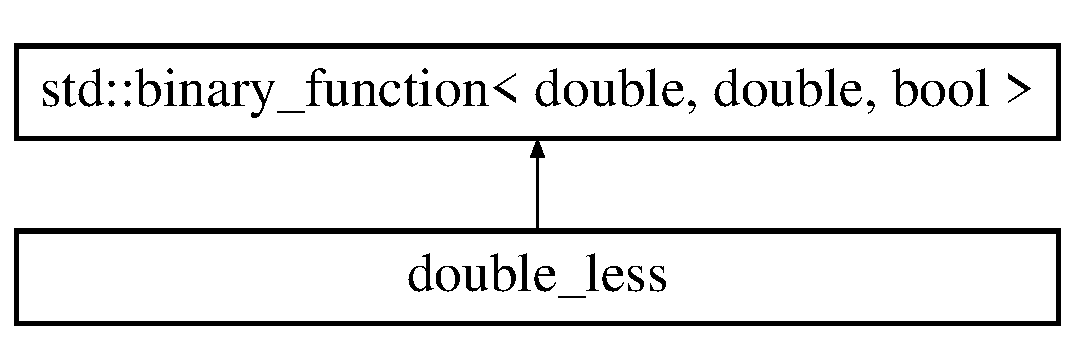
\includegraphics[height=2.000000cm]{classdouble__less}
\end{center}
\end{figure}
\subsection*{Public Member Functions}
\begin{DoxyCompactItemize}
\item 
bool {\bfseries operator()} (const double \&left, const double \&right) const 
\end{DoxyCompactItemize}


\subsection{Detailed Description}
\char`\"{}less\char`\"{} interface for double values. 

The documentation for this class was generated from the following file\+:\begin{DoxyCompactItemize}
\item 
safe\+\_\+math.\+h\end{DoxyCompactItemize}

\section{stemming\+:\+:english\+\_\+stem$<$ string\+\_\+typeT $>$ Class Template Reference}
\label{classstemming_1_1english__stem}\index{stemming\+::english\+\_\+stem$<$ string\+\_\+type\+T $>$@{stemming\+::english\+\_\+stem$<$ string\+\_\+type\+T $>$}}


English stemmer.  




{\ttfamily \#include $<$english\+\_\+stem.\+h$>$}

Inheritance diagram for stemming\+:\+:english\+\_\+stem$<$ string\+\_\+typeT $>$\+:\begin{figure}[H]
\begin{center}
\leavevmode
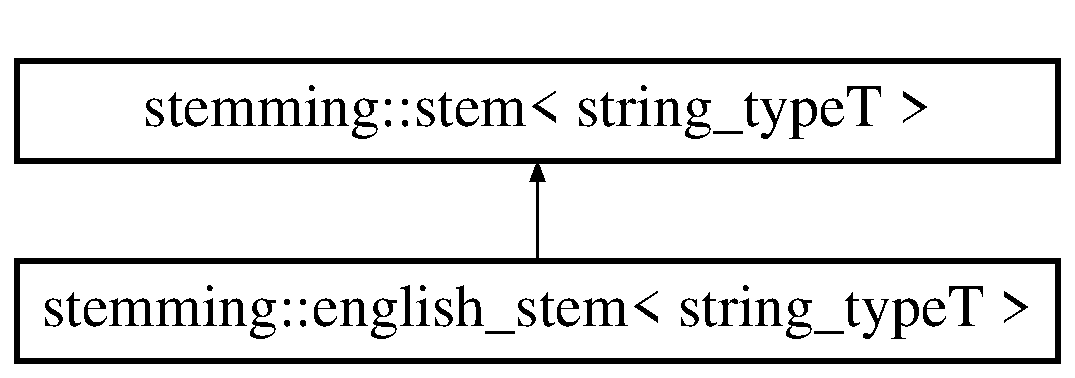
\includegraphics[height=2.000000cm]{classstemming_1_1english__stem}
\end{center}
\end{figure}
\subsection*{Public Member Functions}
\begin{DoxyCompactItemize}
\item 
void {\bf operator()} (string\+\_\+typeT \&text)
\end{DoxyCompactItemize}
\subsection*{Additional Inherited Members}


\subsection{Detailed Description}
\subsubsection*{template$<$typename string\+\_\+typeT = std\+::wstring$>$\\*
class stemming\+::english\+\_\+stem$<$ string\+\_\+type\+T $>$}

English stemmer. 

\begin{DoxyParagraph}{Overview\+:}
I have made more than one attempt to improve the structure of the Porter algorithm by making it follow the pattern of ending removal of the Romance language stemmers. It is not hard to see why one should want to do this\+: step 1b of the Porter stemmer removes ed and ing, which are i-\/suffixes ($\ast$) attached to verbs. If these suffixes are removed, there should be no need to remove d-\/suffixes which are not verbal, although it will try to do so. This seems to be a deficiency in the Porter stemmer, not shared by the Romance stemmers. Again, the divisions between steps 2, 3 and 4 seem rather arbitrary, and are not found in the Romance stemmers. Nevertheless, these attempts at improvement have been abandoned. They seem to lead to a more complicated algorithm with no very obvious improvements. A reason for not taking note of the outcome of step 1b may be that English endings do not determine word categories quite as strongly as endings in the Romance languages. For example, condition and position in French have to be nouns, but in English they can be verbs as well as nouns, We are all conditioned by advertising They are positioning themselves differently today A possible reason for having separate steps 2, 3 and 4 is that d-\/suffix combinations in English are quite complex, a point which has been made elsewhere. But it is hardly surprising that after twenty years of use of the Porter stemmer, certain improvements do suggest themselves, and a new algorithm for English is therefore offered here. (It could be called the \textquotesingle{}Porter2\textquotesingle{} stemmer to distinguish it from the Porter stemmer, from which it derives.) The changes are not so very extensive\+: (1) terminating y is changed to i rather less often, (2) suffix us does not lose its s, (3) a few additional suffixes are included for removal, including (4) suffix ly. In addition, a small list of exceptional forms is included. In December 2001 there were two further adjustments\+: (5) Steps 5a and 5b of the old Porter stemmer were combined into a single step. This means that undoubling final ll is not done with removal of final e. (6) In Step 3 ative is removed only when in region R2. To begin with, here is the basic algorithm without reference to the exceptional forms. An exact comparison with the Porter algorithm needs to be done quite carefully if done at all. Here we indicate by $\ast$ points of departure, and by + additional features. In the sample vocabulary, Porter and Porter2 stem slightly under 5\% of words to different forms. Dr. Martin Porter Define a vowel as one of
\begin{DoxyItemize}
\item a e i o u y Define a double as one of
\item bb dd ff gg mm nn pp rr tt Define a valid li-\/ending as one of
\item c d e g h k m n r t Define a short syllable in a word as either (a) a vowel followed by a non-\/vowel other than w, x or Y and preceded by a non-\/vowel, or $\ast$ (b) a vowel at the beginning of the word followed by a non-\/vowel. So rap, trap, entrap end with a short syllable, and ow, on, at are classed as short syllables. But uproot, bestow, disturb do not end with a short syllable. A word is called short if it consists of a short syllable preceded by zero or more consonants. R1 is the region after the first non-\/vowel following a vowel, or the end of the word if there is no such non-\/vowel. R2 is the region after the first non-\/vowel following a vowel in R1, or the end of the word if there is no such non-\/vowel. If the word has two letters or less, leave it as it is. Otherwise, do each of the following operations, Set initial y, or y after a vowel, to Y, and then establish the regions R1 and R2.
\end{DoxyItemize}
\end{DoxyParagraph}
\begin{DoxyParagraph}{Algorithm\+:}
{\bfseries Step 1a\+:} Search for the longest among the following suffixes, and perform the action indicated\+:
\begin{DoxyItemize}
\item sses
\begin{DoxyItemize}
\item Replace by ss.
\end{DoxyItemize}
\item ied+ ies$\ast$
\begin{DoxyItemize}
\item Replace by i if preceded by just one letter, otherwise by ie (so ties -\/$>$ tie, cries -\/$>$ cri).
\end{DoxyItemize}
\item s
\begin{DoxyItemize}
\item Delete if the preceding word part contains a vowel not immediately before the s (so gas and this retain the s, gaps and kiwis lose it).
\end{DoxyItemize}
\item us+ ss
\begin{DoxyItemize}
\item Do nothing. {\bfseries Step 1b\+:} Search for the longest among the following suffixes, and perform the action indicated\+:
\end{DoxyItemize}
\item eed eedly+
\begin{DoxyItemize}
\item Replace by ee if in R1.
\end{DoxyItemize}
\item ed edly+ ing ingly+
\begin{DoxyItemize}
\item Delete if the preceding word part contains a vowel, and then
\item If the word ends at, bl or iz add e (so luxuriat -\/$>$ luxuriate), or
\item If the word ends with a double remove the last letter (so hopp -\/$>$ hop), or
\item If the word is short, add e (so hop -\/$>$ hope). {\bfseries Step 1c\+:} Replace suffix y or Y by i if preceded by a non-\/vowel which is not the first letter of the word (so cry -\/$>$ cri, by -\/$>$ by, say -\/$>$ say) {\bfseries Step 2\+:} Search for the longest among the following suffixes, and, if found and in R1, perform the action indicated\+:
\end{DoxyItemize}
\item tional
\begin{DoxyItemize}
\item Replace by tion.
\end{DoxyItemize}
\item enci
\begin{DoxyItemize}
\item Replace by ence.
\end{DoxyItemize}
\item anci
\begin{DoxyItemize}
\item Replace by ance
\end{DoxyItemize}
\item abli
\begin{DoxyItemize}
\item Replace by able.
\end{DoxyItemize}
\item entli
\begin{DoxyItemize}
\item Replace by ent.
\end{DoxyItemize}
\item izer ization
\begin{DoxyItemize}
\item Replace by ize.
\end{DoxyItemize}
\item ational ation ator
\begin{DoxyItemize}
\item Replace by ate.
\end{DoxyItemize}
\item alism aliti alli
\begin{DoxyItemize}
\item Replace by al.
\end{DoxyItemize}
\item fulness
\begin{DoxyItemize}
\item Replace by ful.
\end{DoxyItemize}
\item ousli ousness
\begin{DoxyItemize}
\item Replace by ous.
\end{DoxyItemize}
\item iveness iviti
\begin{DoxyItemize}
\item Replace by ive.
\end{DoxyItemize}
\item biliti bli+
\begin{DoxyItemize}
\item Replace by ble.
\end{DoxyItemize}
\item ogi+
\begin{DoxyItemize}
\item Replace by og if preceded by l.
\end{DoxyItemize}
\item fulli+
\begin{DoxyItemize}
\item Replace by ful.
\end{DoxyItemize}
\item lessli+
\begin{DoxyItemize}
\item Replace by less.
\end{DoxyItemize}
\item li+
\begin{DoxyItemize}
\item Delete if preceded by a valid li-\/ending. {\bfseries Step 3\+:} Search for the longest among the following suffixes, and, if found and in R1, perform the action indicated\+:
\end{DoxyItemize}
\item tional+
\begin{DoxyItemize}
\item Replace by tion.
\end{DoxyItemize}
\item ational+
\begin{DoxyItemize}
\item Replace by ate.
\end{DoxyItemize}
\item alize
\begin{DoxyItemize}
\item Replace by al.
\end{DoxyItemize}
\item icate iciti ical
\begin{DoxyItemize}
\item Replace by ic.
\end{DoxyItemize}
\item ful ness
\begin{DoxyItemize}
\item Delete.
\end{DoxyItemize}
\item ative$\ast$
\begin{DoxyItemize}
\item Delete if in R2. {\bfseries Step 4\+:} Search for the longest among the following suffixes, and, if found and in R2, perform the action indicated\+:
\end{DoxyItemize}
\item al ance ence er ic able ible ant ement ment ent ism ate iti ous ive ize
\begin{DoxyItemize}
\item Delete
\end{DoxyItemize}
\item ion
\begin{DoxyItemize}
\item Delete if preceded by s or t. {\bfseries Step 5\+:} Search for the following suffixes, and, if found, perform the action indicated\+:
\end{DoxyItemize}
\item e
\begin{DoxyItemize}
\item Delete if in R2, or in R1 and not preceded by a short syllable.
\end{DoxyItemize}
\item l
\begin{DoxyItemize}
\item Delete if in R2 and preceded by l. 
\end{DoxyItemize}
\end{DoxyItemize}
\end{DoxyParagraph}


\subsection{Member Function Documentation}
\index{stemming\+::english\+\_\+stem@{stemming\+::english\+\_\+stem}!operator()@{operator()}}
\index{operator()@{operator()}!stemming\+::english\+\_\+stem@{stemming\+::english\+\_\+stem}}
\subsubsection[{operator()(string\+\_\+type\+T \&text)}]{\setlength{\rightskip}{0pt plus 5cm}template$<$typename string\+\_\+typeT  = std\+::wstring$>$ void {\bf stemming\+::english\+\_\+stem}$<$ string\+\_\+typeT $>$\+::operator() (
\begin{DoxyParamCaption}
\item[{string\+\_\+typeT \&}]{text}
\end{DoxyParamCaption}
)\hspace{0.3cm}{\ttfamily [inline]}}\label{classstemming_1_1english__stem_a8163a8cc4186b749665d616cbf11c492}

\begin{DoxyParams}[1]{Parameters}
\mbox{\tt in,out}  & {\em text} & English string to stem. \\
\hline
\end{DoxyParams}


The documentation for this class was generated from the following file\+:\begin{DoxyCompactItemize}
\item 
/home/coder/\+C\+S\+E2341-\/17\+S-\/\+Lose-\/lose-\/situation/\+F\+Project/english\+\_\+stem.\+h\end{DoxyCompactItemize}

\section{string\+\_\+util\+:\+:equal\+\_\+basic\+\_\+string\+\_\+i\+\_\+compare$<$ T $>$ Class Template Reference}
\label{classstring__util_1_1equal__basic__string__i__compare}\index{string\+\_\+util\+::equal\+\_\+basic\+\_\+string\+\_\+i\+\_\+compare$<$ T $>$@{string\+\_\+util\+::equal\+\_\+basic\+\_\+string\+\_\+i\+\_\+compare$<$ T $>$}}


Inheritance diagram for string\+\_\+util\+:\+:equal\+\_\+basic\+\_\+string\+\_\+i\+\_\+compare$<$ T $>$\+:
% FIG 0


Collaboration diagram for string\+\_\+util\+:\+:equal\+\_\+basic\+\_\+string\+\_\+i\+\_\+compare$<$ T $>$\+:
% FIG 1
\subsection*{Public Member Functions}
\begin{DoxyCompactItemize}
\item 
bool {\bfseries operator()} (const T \&a\+\_\+, const T \&b\+\_\+) const \label{classstring__util_1_1equal__basic__string__i__compare_a29fabe519d28908f5b72dcb799cac64f}

\end{DoxyCompactItemize}


The documentation for this class was generated from the following file\+:\begin{DoxyCompactItemize}
\item 
string\+\_\+util.\+h\end{DoxyCompactItemize}

\section{string\+\_\+util\+:\+:equal\+\_\+string\+\_\+compare$<$ T $>$ Class Template Reference}
\label{classstring__util_1_1equal__string__compare}\index{string\+\_\+util\+::equal\+\_\+string\+\_\+compare$<$ T $>$@{string\+\_\+util\+::equal\+\_\+string\+\_\+compare$<$ T $>$}}


Inheritance diagram for string\+\_\+util\+:\+:equal\+\_\+string\+\_\+compare$<$ T $>$\+:
% FIG 0


Collaboration diagram for string\+\_\+util\+:\+:equal\+\_\+string\+\_\+compare$<$ T $>$\+:
% FIG 1
\subsection*{Public Member Functions}
\begin{DoxyCompactItemize}
\item 
bool {\bfseries operator()} (const T $\ast$a\+\_\+, const T $\ast$b\+\_\+) const \label{classstring__util_1_1equal__string__compare_aedfb40c0515b97043369af03da1d72ed}

\end{DoxyCompactItemize}


The documentation for this class was generated from the following file\+:\begin{DoxyCompactItemize}
\item 
string\+\_\+util.\+h\end{DoxyCompactItemize}

\section{string\+\_\+util\+:\+:equal\+\_\+string\+\_\+i\+\_\+compare$<$ T $>$ Class Template Reference}
\label{classstring__util_1_1equal__string__i__compare}\index{string\+\_\+util\+::equal\+\_\+string\+\_\+i\+\_\+compare$<$ T $>$@{string\+\_\+util\+::equal\+\_\+string\+\_\+i\+\_\+compare$<$ T $>$}}
Inheritance diagram for string\+\_\+util\+:\+:equal\+\_\+string\+\_\+i\+\_\+compare$<$ T $>$\+:\begin{figure}[H]
\begin{center}
\leavevmode
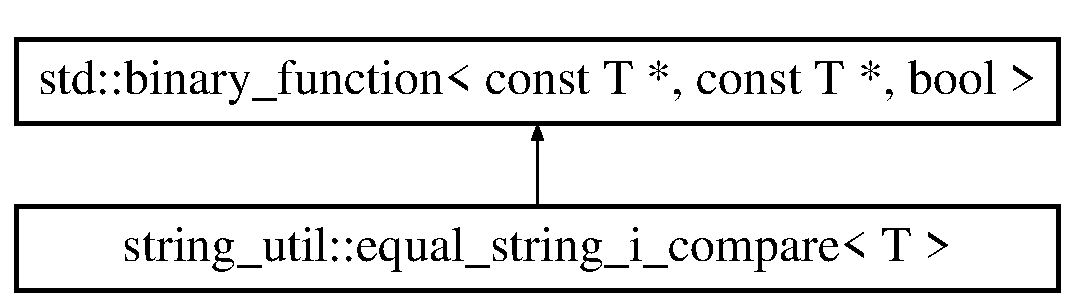
\includegraphics[height=2.000000cm]{classstring__util_1_1equal__string__i__compare}
\end{center}
\end{figure}
\subsection*{Public Member Functions}
\begin{DoxyCompactItemize}
\item 
bool {\bfseries operator()} (const T $\ast$a\+\_\+, const T $\ast$b\+\_\+) const \label{classstring__util_1_1equal__string__i__compare_af8c94159bbb8903c7cf7b71941a7d2bc}

\end{DoxyCompactItemize}


The documentation for this class was generated from the following file\+:\begin{DoxyCompactItemize}
\item 
/home/coder/\+C\+S\+E2341-\/17\+S-\/\+Lose-\/lose-\/situation/\+F\+Project/string\+\_\+util.\+h\end{DoxyCompactItemize}

\section{hashy Class Reference}
\label{classhashy}\index{hashy@{hashy}}
Inheritance diagram for hashy\+:\begin{figure}[H]
\begin{center}
\leavevmode
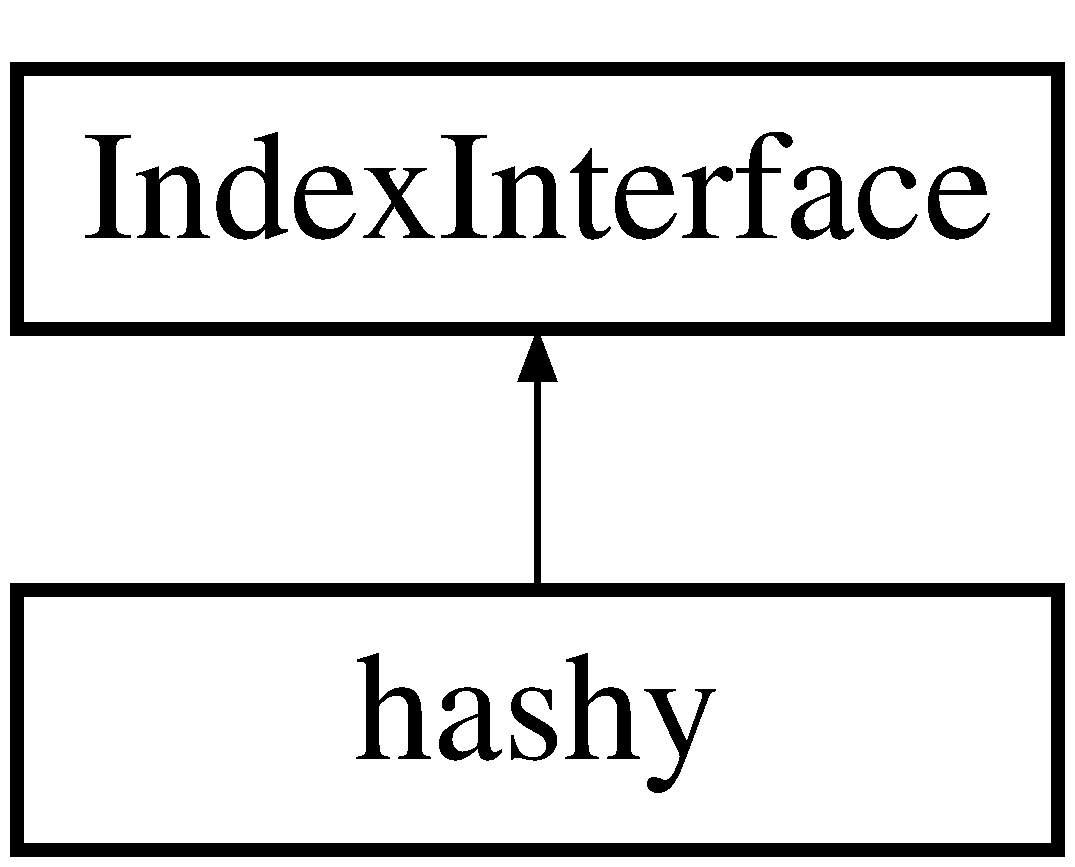
\includegraphics[height=2.000000cm]{classhashy}
\end{center}
\end{figure}
\subsection*{Public Member Functions}
\begin{DoxyCompactItemize}
\item 
{\bf hashy} ()\label{classhashy_ab050f001c1a89c1e15fb1739626c8951}

\begin{DoxyCompactList}\small\item\em This is the constructor for the custom hash table. \end{DoxyCompactList}\item 
int {\bf Hashy} (string key)
\begin{DoxyCompactList}\small\item\em Hashy. \end{DoxyCompactList}\item 
void {\bfseries add\+Index} (string \&word, string \&name)\label{classhashy_ab6e0bf2ad21ff3ecfb313fdb0ad5c8f0}

\item 
int {\bfseries Num\+Items\+In\+Index} (int index)\label{classhashy_aeeb63d39a0c003a2a9b8c21dc6025621}

\item 
void {\bfseries display} ()\label{classhashy_aa45c52806c5d41632dfd06f981d2f077}

\item 
void {\bfseries display\+Index} (int index)\label{classhashy_a4d6553a650fa179be75d43d6bf0937a8}

\item 
vector$<$ {\bf document} $>$ $\ast$ {\bfseries find\+Index} (string word)\label{classhashy_a1896f27d06ef1312b49d6756b7df9886}

\item 
virtual void {\bfseries read\+Index} ()\label{classhashy_a967409a70ff79b9e327bd199144ff974}

\item 
virtual void {\bfseries write\+Index} ()\label{classhashy_a9eee50b1514d733aad262ae74b190121}

\item 
virtual void {\bfseries insert\+From\+File} (string \&word, string \&doc, int \&count)\label{classhashy_a83616aa2459834e846439b8c11895a6a}

\item 
vector$<$ std\+::string $>$ {\bfseries split} (const std\+::string \&s, char delim)\label{classhashy_a5241877dd707ededf7023bae50fa17d6}

\item 
virtual vector$<$ {\bf document} $>$ {\bfseries topwords} ()\label{classhashy_adbe9acb0d7ab3caaf956f61b1f93bb2c}

\item 
virtual int {\bfseries total\+Words\+Indexed} ()\label{classhashy_ab763dc0125d94ed8f54bc83c8821f71e}

\end{DoxyCompactItemize}


\subsection{Member Function Documentation}
\index{hashy@{hashy}!Hashy@{Hashy}}
\index{Hashy@{Hashy}!hashy@{hashy}}
\subsubsection[{Hashy(string key)}]{\setlength{\rightskip}{0pt plus 5cm}int hashy\+::\+Hashy (
\begin{DoxyParamCaption}
\item[{string}]{key}
\end{DoxyParamCaption}
)}\label{classhashy_ae7ff1a1b27254330aa13d815bd12c885}


Hashy. 


\begin{DoxyParams}{Parameters}
{\em word} & key \\
\hline
\end{DoxyParams}
\begin{DoxyReturn}{Returns}
int 
\end{DoxyReturn}


The documentation for this class was generated from the following files\+:\begin{DoxyCompactItemize}
\item 
hash.\+h\item 
hash.\+cpp\end{DoxyCompactItemize}

\section{index\+\_\+node Struct Reference}
\label{structindex__node}\index{index\+\_\+node@{index\+\_\+node}}
\subsection*{Public Attributes}
\begin{DoxyCompactItemize}
\item 
string {\bfseries word\+\_\+key}\label{structindex__node_a1a2e9b2dbf3e0208a16f4ca907c9e578}

\item 
{\bf index\+\_\+node} $\ast$ {\bfseries left}\label{structindex__node_a45b8fb67fb23923d9201a838d0afa54e}

\item 
{\bf index\+\_\+node} $\ast$ {\bfseries right}\label{structindex__node_a79288aaf4380e0689ba1191f632f1919}

\item 
vector$<$ {\bf document} $>$ {\bfseries documents}\label{structindex__node_ac30a2d3c128b8a88193eccf05efd1ba2}

\item 
int {\bfseries height}\label{structindex__node_a711a4ee7677aec85f96014f5b44dacd7}

\end{DoxyCompactItemize}


The documentation for this struct was generated from the following file\+:\begin{DoxyCompactItemize}
\item 
avltreeindex.\+h\end{DoxyCompactItemize}

\section{indexextractor Class Reference}
\label{classindexextractor}\index{indexextractor@{indexextractor}}


The indexextractor class.  




{\ttfamily \#include $<$indexextractor.\+h$>$}

\subsection*{Public Member Functions}
\begin{DoxyCompactItemize}
\item 
{\bf indexextractor} (string)
\begin{DoxyCompactList}\small\item\em The Index\+Extractor class stems the words and removes stopwords. The code makes use of the .......... \end{DoxyCompactList}\item 
void {\bf use\+Stop\+Words} (string)\label{classindexextractor_a8b235e64a7c1fa2b73be3b87dce8d1f5}

\begin{DoxyCompactList}\small\item\em \doxyref{indexextractor\+::use\+Stop\+Words}{p.}{classindexextractor_a8b235e64a7c1fa2b73be3b87dce8d1f5} adds the stop words from a file \end{DoxyCompactList}\item 
bool {\bf is\+Stop\+Word} (string \&)\label{classindexextractor_a7f0d3c2aedcdeee8b3797582e06bfefc}

\begin{DoxyCompactList}\small\item\em \doxyref{indexextractor\+::is\+Stop\+Word}{p.}{classindexextractor_a7f0d3c2aedcdeee8b3797582e06bfefc} This checks if it is in the stop words set \end{DoxyCompactList}\item 
string {\bf get\+Stemmed} (string \&)\label{classindexextractor_a5b6ed2949c02655b2fd4e0204ed31a25}

\begin{DoxyCompactList}\small\item\em \doxyref{indexextractor\+::get\+Stemmed}{p.}{classindexextractor_a5b6ed2949c02655b2fd4e0204ed31a25} This gets the stemmed version of the word \end{DoxyCompactList}\end{DoxyCompactItemize}


\subsection{Detailed Description}
The indexextractor class. 

\subsection{Constructor \& Destructor Documentation}
\index{indexextractor@{indexextractor}!indexextractor@{indexextractor}}
\index{indexextractor@{indexextractor}!indexextractor@{indexextractor}}
\subsubsection[{indexextractor(string)}]{\setlength{\rightskip}{0pt plus 5cm}indexextractor\+::indexextractor (
\begin{DoxyParamCaption}
\item[{string}]{stoptxt}
\end{DoxyParamCaption}
)}\label{classindexextractor_a650a58859c23488d46e47a377766b560}


The Index\+Extractor class stems the words and removes stopwords. The code makes use of the .......... 

C\+SE 2341 Index\+Extractor.\+cpp \begin{DoxyAuthor}{Author}
Aviraj Shina (owner) 
\end{DoxyAuthor}
\begin{DoxyVersion}{Version}
1.\+0 05/07/17 \doxyref{indexextractor\+::indexextractor}{p.}{classindexextractor_a650a58859c23488d46e47a377766b560} This class is repsonsible for stemming and stop words 
\end{DoxyVersion}


The documentation for this class was generated from the following files\+:\begin{DoxyCompactItemize}
\item 
indexextractor.\+h\item 
indexextractor.\+cpp\end{DoxyCompactItemize}

\section{Index\+Handler Class Reference}
\label{class_index_handler}\index{Index\+Handler@{Index\+Handler}}


The \doxyref{Index\+Handler}{p.}{class_index_handler} class.  




{\ttfamily \#include $<$indexhandler.\+h$>$}

\subsection*{Public Member Functions}
\begin{DoxyCompactItemize}
\item 
{\bf Index\+Handler} (char type)
\begin{DoxyCompactList}\small\item\em The \doxyref{Index\+Handler}{p.}{class_index_handler} class creates and stores the inverted index file. It uses the custom data structures to write and read the inverted index. \end{DoxyCompactList}\item 
void {\bf write\+Index} ()\label{class_index_handler_af4e152fb943fc9fd3962e008bd9e6ea5}

\begin{DoxyCompactList}\small\item\em \doxyref{Index\+Handler\+::write\+Index}{p.}{class_index_handler_af4e152fb943fc9fd3962e008bd9e6ea5} This writes the inverted index file to the .txt file from the appropriate data structure. \end{DoxyCompactList}\item 
void {\bf add\+Index} (string, string)
\begin{DoxyCompactList}\small\item\em \doxyref{Index\+Handler\+::add\+Index}{p.}{class_index_handler_ad4bfa5c8de41b1b32a46db8094510d46} This adds the word and the P\+Df name to the chosen data structure. \end{DoxyCompactList}\item 
vector$<$ {\bf document} $>$ $\ast$ {\bf get\+Docs} (string)
\begin{DoxyCompactList}\small\item\em \doxyref{Index\+Handler\+::get\+Docs}{p.}{class_index_handler_a8d4cdec1dd190ba28dc8e743333ca597} This returns the name of all of the P\+D\+Fs containing the requested word. \end{DoxyCompactList}\item 
int {\bfseries get\+Document\+Frequency} (string word, string docname)\label{class_index_handler_adba159334381d1fa51741defbeaa7a34}

\item 
int {\bfseries get\+Corpus\+Frequency} (string word)\label{class_index_handler_a64ed60231ddbd004bef0a8b36a941947}

\item 
void {\bf display\+Indices} ()\label{class_index_handler_a62629856602056eea2172d8c207fb4de}

\begin{DoxyCompactList}\small\item\em \doxyref{Index\+Handler\+::display\+Indices}{p.}{class_index_handler_a62629856602056eea2172d8c207fb4de} This dispays the indicies of the appropriate data structure. \end{DoxyCompactList}\item 
void {\bf read\+Index} ()\label{class_index_handler_a8a0cd8e4f2fe194a5ab11ab2922c39a4}

\begin{DoxyCompactList}\small\item\em \doxyref{Index\+Handler\+::read\+Index}{p.}{class_index_handler_a8a0cd8e4f2fe194a5ab11ab2922c39a4} This reads the data from the inverted index file and into the appropriate data structure. \end{DoxyCompactList}\item 
vector$<$ {\bf document} $>$ {\bf top\+Fifty} ()
\begin{DoxyCompactList}\small\item\em \doxyref{Index\+Handler\+::top\+Fifty}{p.}{class_index_handler_acbcc15002e12ab79d6fe05d7e8dc8833} This returns the top fifty words and their count. \end{DoxyCompactList}\item 
int {\bf total\+Words\+Indexed} ()
\begin{DoxyCompactList}\small\item\em \doxyref{Index\+Handler\+::total\+Words\+Indexed}{p.}{class_index_handler_ab23ff6f1883b84bb7fa8732e598ac403} This returns the total number of words indexed. \end{DoxyCompactList}\end{DoxyCompactItemize}


\subsection{Detailed Description}
The \doxyref{Index\+Handler}{p.}{class_index_handler} class. 

\subsection{Constructor \& Destructor Documentation}
\index{Index\+Handler@{Index\+Handler}!Index\+Handler@{Index\+Handler}}
\index{Index\+Handler@{Index\+Handler}!Index\+Handler@{Index\+Handler}}
\subsubsection[{Index\+Handler(char type)}]{\setlength{\rightskip}{0pt plus 5cm}Index\+Handler\+::\+Index\+Handler (
\begin{DoxyParamCaption}
\item[{char}]{type}
\end{DoxyParamCaption}
)}\label{class_index_handler_a222c2e9f12fef0e242c7870836df88e8}


The \doxyref{Index\+Handler}{p.}{class_index_handler} class creates and stores the inverted index file. It uses the custom data structures to write and read the inverted index. 

C\+SE 2341 Index\+Handler.\+h \begin{DoxyAuthor}{Author}
Aviraj Shina (owner) 

Patrick Yienger 
\end{DoxyAuthor}
\begin{DoxyVersion}{Version}
1.\+0 05/07/17 \doxyref{Index\+Handler\+::\+Index\+Handler}{p.}{class_index_handler_a222c2e9f12fef0e242c7870836df88e8} The index handler constructor. This initialaizes the chosen data structure. 
\end{DoxyVersion}

\begin{DoxyParams}{Parameters}
{\em type} & The data structure to be initalized. \\
\hline
\end{DoxyParams}


\subsection{Member Function Documentation}
\index{Index\+Handler@{Index\+Handler}!add\+Index@{add\+Index}}
\index{add\+Index@{add\+Index}!Index\+Handler@{Index\+Handler}}
\subsubsection[{add\+Index(string, string)}]{\setlength{\rightskip}{0pt plus 5cm}void Index\+Handler\+::add\+Index (
\begin{DoxyParamCaption}
\item[{string}]{word, }
\item[{string}]{docname}
\end{DoxyParamCaption}
)}\label{class_index_handler_ad4bfa5c8de41b1b32a46db8094510d46}


\doxyref{Index\+Handler\+::add\+Index}{p.}{class_index_handler_ad4bfa5c8de41b1b32a46db8094510d46} This adds the word and the P\+Df name to the chosen data structure. 


\begin{DoxyParams}{Parameters}
{\em word} & The word to be added. \\
\hline
{\em docname} & The P\+DF name to be added. \\
\hline
\end{DoxyParams}
\index{Index\+Handler@{Index\+Handler}!get\+Docs@{get\+Docs}}
\index{get\+Docs@{get\+Docs}!Index\+Handler@{Index\+Handler}}
\subsubsection[{get\+Docs(string)}]{\setlength{\rightskip}{0pt plus 5cm}vector$<$ {\bf document} $>$ $\ast$ Index\+Handler\+::get\+Docs (
\begin{DoxyParamCaption}
\item[{string}]{word}
\end{DoxyParamCaption}
)}\label{class_index_handler_a8d4cdec1dd190ba28dc8e743333ca597}


\doxyref{Index\+Handler\+::get\+Docs}{p.}{class_index_handler_a8d4cdec1dd190ba28dc8e743333ca597} This returns the name of all of the P\+D\+Fs containing the requested word. 


\begin{DoxyParams}{Parameters}
{\em word} & The word requested. \\
\hline
\end{DoxyParams}
\begin{DoxyReturn}{Returns}
vector$<$document$>$ The vector of document object that stores the count and P\+DF name of the requested word. 
\end{DoxyReturn}
\index{Index\+Handler@{Index\+Handler}!top\+Fifty@{top\+Fifty}}
\index{top\+Fifty@{top\+Fifty}!Index\+Handler@{Index\+Handler}}
\subsubsection[{top\+Fifty()}]{\setlength{\rightskip}{0pt plus 5cm}vector$<$ {\bf document} $>$ Index\+Handler\+::top\+Fifty (
\begin{DoxyParamCaption}
{}
\end{DoxyParamCaption}
)}\label{class_index_handler_acbcc15002e12ab79d6fe05d7e8dc8833}


\doxyref{Index\+Handler\+::top\+Fifty}{p.}{class_index_handler_acbcc15002e12ab79d6fe05d7e8dc8833} This returns the top fifty words and their count. 

\begin{DoxyReturn}{Returns}
vector$<$document$>$ This returns the vector of document objects containing the word and the count. 
\end{DoxyReturn}
\index{Index\+Handler@{Index\+Handler}!total\+Words\+Indexed@{total\+Words\+Indexed}}
\index{total\+Words\+Indexed@{total\+Words\+Indexed}!Index\+Handler@{Index\+Handler}}
\subsubsection[{total\+Words\+Indexed()}]{\setlength{\rightskip}{0pt plus 5cm}int Index\+Handler\+::total\+Words\+Indexed (
\begin{DoxyParamCaption}
{}
\end{DoxyParamCaption}
)}\label{class_index_handler_ab23ff6f1883b84bb7fa8732e598ac403}


\doxyref{Index\+Handler\+::total\+Words\+Indexed}{p.}{class_index_handler_ab23ff6f1883b84bb7fa8732e598ac403} This returns the total number of words indexed. 

\begin{DoxyReturn}{Returns}
total\+Words\+Indexed 
\end{DoxyReturn}


The documentation for this class was generated from the following files\+:\begin{DoxyCompactItemize}
\item 
/home/coder/\+C\+S\+E2341-\/17\+S-\/\+Lose-\/lose-\/situation/\+F\+Project/indexhandler.\+h\item 
/home/coder/\+C\+S\+E2341-\/17\+S-\/\+Lose-\/lose-\/situation/\+F\+Project/indexhandler.\+cpp\end{DoxyCompactItemize}

\section{Index\+Interface Class Reference}
\label{class_index_interface}\index{Index\+Interface@{Index\+Interface}}
Inheritance diagram for Index\+Interface\+:\begin{figure}[H]
\begin{center}
\leavevmode
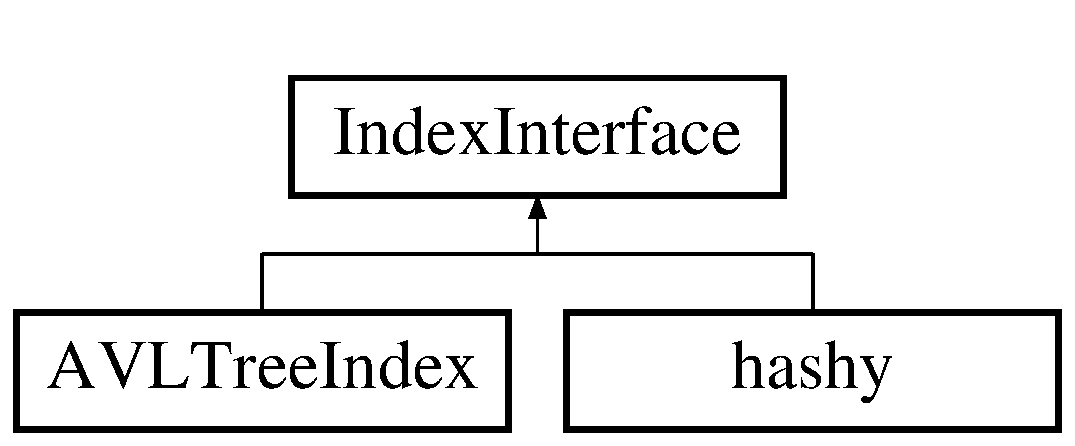
\includegraphics[height=2.000000cm]{class_index_interface}
\end{center}
\end{figure}
\subsection*{Public Member Functions}
\begin{DoxyCompactItemize}
\item 
virtual vector$<$ {\bf document} $>$ $\ast$ {\bfseries find\+Index} (string key)=0\label{class_index_interface_a2f50625affbeda31e1314664f4a1af98}

\item 
virtual void {\bfseries add\+Index} (string \&word, string \&doc)=0\label{class_index_interface_ae3a511e458f11529f3c8cb82dcf81e23}

\item 
virtual void {\bfseries display} ()=0\label{class_index_interface_a09a2aef2e093bf1d4b34bffa89382aa5}

\item 
virtual void {\bfseries read\+Index} ()=0\label{class_index_interface_ab17e509ad40bfc8c0f90e8382c8e9931}

\item 
virtual void {\bfseries write\+Index} ()=0\label{class_index_interface_a6d924312167449866fdc747839cc37eb}

\item 
virtual vector$<$ {\bf document} $>$ {\bfseries topwords} ()=0\label{class_index_interface_ac48997ed829d72743a7d96f95d6c69fe}

\item 
virtual int {\bfseries total\+Words\+Indexed} ()=0\label{class_index_interface_a5a267a6d18eb64b8d5928b1c3e9f8cd9}

\end{DoxyCompactItemize}


The documentation for this class was generated from the following file\+:\begin{DoxyCompactItemize}
\item 
indexinterface.\+h\end{DoxyCompactItemize}

\section{item Struct Reference}
\label{structitem}\index{item@{item}}


The hashy class is the custom implementation of the Hash\+Table. The basic hash parts of the code was based off of the series of videos by Paul Programming.  




{\ttfamily \#include $<$hash.\+h$>$}

\subsection*{Public Attributes}
\begin{DoxyCompactItemize}
\item 
string {\bfseries word\+\_\+key}\label{structitem_ac8277a05ff6123953e155ce6509abfbb}

\item 
int {\bfseries count}\label{structitem_a84ad511a7e7fc725743a4399fa240c61}

\item 
string {\bfseries doc\+Name}\label{structitem_ab0e6ffba7b90e2d2f248eb89ec245e75}

\item 
vector$<$ {\bf item} $>$ {\bfseries vec}\label{structitem_a9cfe089919ee381e330a884914751bff}

\end{DoxyCompactItemize}


\subsection{Detailed Description}
The hashy class is the custom implementation of the Hash\+Table. The basic hash parts of the code was based off of the series of videos by Paul Programming. 

C\+SE 2341 \doxyref{hash.\+h}{p.}{hash_8h_source} \begin{DoxyAuthor}{Author}
Parick Yienger (owner) 
\end{DoxyAuthor}
\begin{DoxyVersion}{Version}
1.\+0 05/07/17 The item struct This is a struct that contains the word, count, and P\+D\+F\+Name. It also uses a vector in the top index on the hash table to handle collisions. 
\end{DoxyVersion}


The documentation for this struct was generated from the following file\+:\begin{DoxyCompactItemize}
\item 
hash.\+h\end{DoxyCompactItemize}

\section{string\+\_\+util\+:\+:less\+\_\+basic\+\_\+string\+\_\+compare$<$ T $>$ Class Template Reference}
\label{classstring__util_1_1less__basic__string__compare}\index{string\+\_\+util\+::less\+\_\+basic\+\_\+string\+\_\+compare$<$ T $>$@{string\+\_\+util\+::less\+\_\+basic\+\_\+string\+\_\+compare$<$ T $>$}}
Inheritance diagram for string\+\_\+util\+:\+:less\+\_\+basic\+\_\+string\+\_\+compare$<$ T $>$\+:\begin{figure}[H]
\begin{center}
\leavevmode
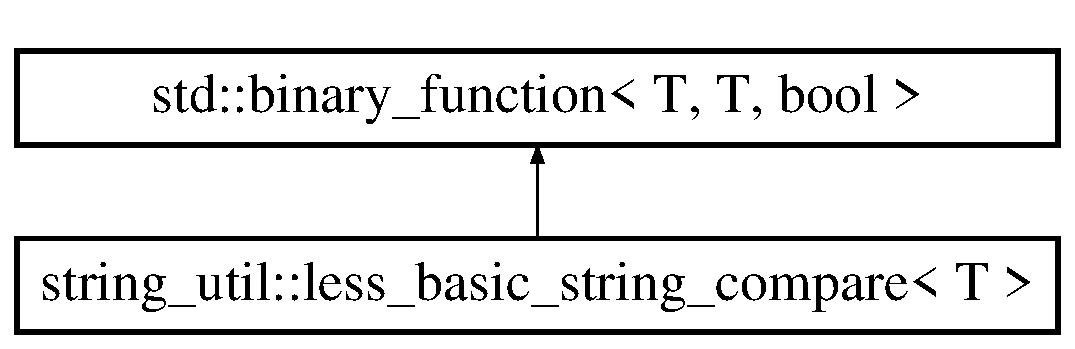
\includegraphics[height=2.000000cm]{classstring__util_1_1less__basic__string__compare}
\end{center}
\end{figure}
\subsection*{Public Member Functions}
\begin{DoxyCompactItemize}
\item 
bool {\bfseries operator()} (const T \&a\+\_\+, const T \&b\+\_\+) const \label{classstring__util_1_1less__basic__string__compare_a259341e58f36d8aaf75f2415de0df4d8}

\end{DoxyCompactItemize}


The documentation for this class was generated from the following file\+:\begin{DoxyCompactItemize}
\item 
/home/coder/\+C\+S\+E2341-\/17\+S-\/\+Lose-\/lose-\/situation/\+F\+Project/string\+\_\+util.\+h\end{DoxyCompactItemize}

\section{string\+\_\+util\+:\+:less\+\_\+string\+\_\+compare$<$ T $>$ Class Template Reference}
\label{classstring__util_1_1less__string__compare}\index{string\+\_\+util\+::less\+\_\+string\+\_\+compare$<$ T $>$@{string\+\_\+util\+::less\+\_\+string\+\_\+compare$<$ T $>$}}


Inheritance diagram for string\+\_\+util\+:\+:less\+\_\+string\+\_\+compare$<$ T $>$\+:
% FIG 0


Collaboration diagram for string\+\_\+util\+:\+:less\+\_\+string\+\_\+compare$<$ T $>$\+:
% FIG 1
\subsection*{Public Member Functions}
\begin{DoxyCompactItemize}
\item 
bool {\bfseries operator()} (const T $\ast$a\+\_\+, const T $\ast$b\+\_\+) const \label{classstring__util_1_1less__string__compare_aa97df82edd8f7e33e5715acf71759337}

\end{DoxyCompactItemize}


The documentation for this class was generated from the following file\+:\begin{DoxyCompactItemize}
\item 
string\+\_\+util.\+h\end{DoxyCompactItemize}

\section{string\+\_\+util\+:\+:less\+\_\+string\+\_\+i\+\_\+compare$<$ T $>$ Class Template Reference}
\label{classstring__util_1_1less__string__i__compare}\index{string\+\_\+util\+::less\+\_\+string\+\_\+i\+\_\+compare$<$ T $>$@{string\+\_\+util\+::less\+\_\+string\+\_\+i\+\_\+compare$<$ T $>$}}
Inheritance diagram for string\+\_\+util\+:\+:less\+\_\+string\+\_\+i\+\_\+compare$<$ T $>$\+:\begin{figure}[H]
\begin{center}
\leavevmode
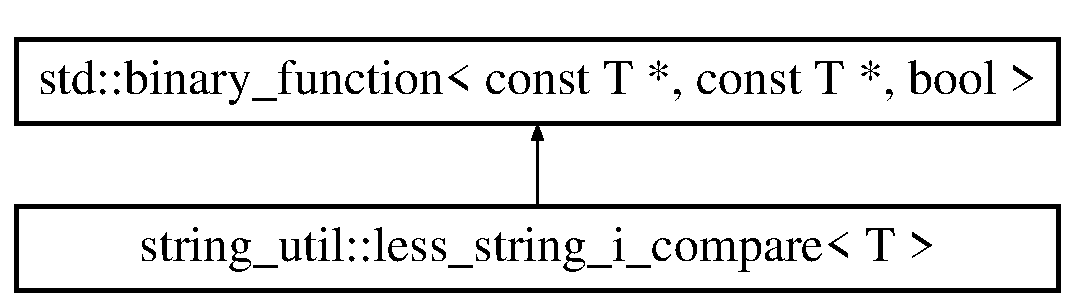
\includegraphics[height=2.000000cm]{classstring__util_1_1less__string__i__compare}
\end{center}
\end{figure}
\subsection*{Public Member Functions}
\begin{DoxyCompactItemize}
\item 
bool {\bfseries operator()} (const T $\ast$a\+\_\+, const T $\ast$b\+\_\+) const \label{classstring__util_1_1less__string__i__compare_ae2dd6a625b07bc51060805b30e7547a1}

\end{DoxyCompactItemize}


The documentation for this class was generated from the following file\+:\begin{DoxyCompactItemize}
\item 
string\+\_\+util.\+h\end{DoxyCompactItemize}

\section{string\+\_\+util\+:\+:less\+\_\+string\+\_\+n\+\_\+compare$<$ T $>$ Class Template Reference}
\label{classstring__util_1_1less__string__n__compare}\index{string\+\_\+util\+::less\+\_\+string\+\_\+n\+\_\+compare$<$ T $>$@{string\+\_\+util\+::less\+\_\+string\+\_\+n\+\_\+compare$<$ T $>$}}
Inheritance diagram for string\+\_\+util\+:\+:less\+\_\+string\+\_\+n\+\_\+compare$<$ T $>$\+:\begin{figure}[H]
\begin{center}
\leavevmode
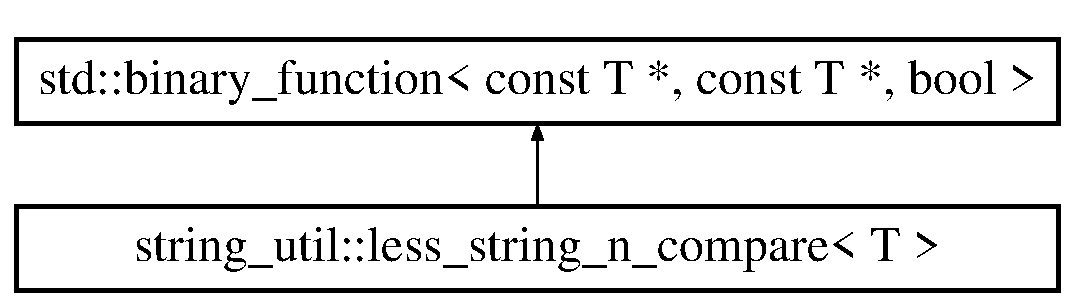
\includegraphics[height=2.000000cm]{classstring__util_1_1less__string__n__compare}
\end{center}
\end{figure}
\subsection*{Public Member Functions}
\begin{DoxyCompactItemize}
\item 
{\bfseries less\+\_\+string\+\_\+n\+\_\+compare} (size\+\_\+t comparison\+\_\+size)\label{classstring__util_1_1less__string__n__compare_a42b269c0aa27c5ace8b3eeb782f6d335}

\item 
bool {\bfseries operator()} (const T $\ast$a\+\_\+, const T $\ast$b\+\_\+) const \label{classstring__util_1_1less__string__n__compare_ab6f6bb1fbd6421cb848bba88ce18f6e0}

\end{DoxyCompactItemize}


The documentation for this class was generated from the following file\+:\begin{DoxyCompactItemize}
\item 
/home/coder/\+C\+S\+E2341-\/17\+S-\/\+Lose-\/lose-\/situation/\+F\+Project/string\+\_\+util.\+h\end{DoxyCompactItemize}

\section{string\+\_\+util\+:\+:less\+\_\+string\+\_\+natural\+\_\+order\+\_\+i\+\_\+compare$<$ T $>$ Class Template Reference}
\label{classstring__util_1_1less__string__natural__order__i__compare}\index{string\+\_\+util\+::less\+\_\+string\+\_\+natural\+\_\+order\+\_\+i\+\_\+compare$<$ T $>$@{string\+\_\+util\+::less\+\_\+string\+\_\+natural\+\_\+order\+\_\+i\+\_\+compare$<$ T $>$}}
Inheritance diagram for string\+\_\+util\+:\+:less\+\_\+string\+\_\+natural\+\_\+order\+\_\+i\+\_\+compare$<$ T $>$\+:\begin{figure}[H]
\begin{center}
\leavevmode
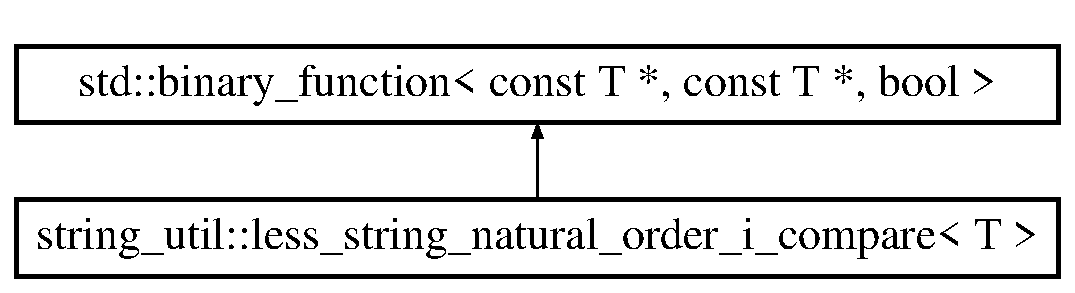
\includegraphics[height=2.000000cm]{classstring__util_1_1less__string__natural__order__i__compare}
\end{center}
\end{figure}
\subsection*{Public Member Functions}
\begin{DoxyCompactItemize}
\item 
bool {\bfseries operator()} (const T $\ast$a\+\_\+, const T $\ast$b\+\_\+) const \label{classstring__util_1_1less__string__natural__order__i__compare_a213ba84bcb81fa025951194acbdb899c}

\end{DoxyCompactItemize}


The documentation for this class was generated from the following file\+:\begin{DoxyCompactItemize}
\item 
/home/coder/\+C\+S\+E2341-\/17\+S-\/\+Lose-\/lose-\/situation/\+F\+Project/string\+\_\+util.\+h\end{DoxyCompactItemize}

\section{string\+\_\+util\+:\+:less\+\_\+string\+\_\+ni\+\_\+compare$<$ T $>$ Class Template Reference}
\label{classstring__util_1_1less__string__ni__compare}\index{string\+\_\+util\+::less\+\_\+string\+\_\+ni\+\_\+compare$<$ T $>$@{string\+\_\+util\+::less\+\_\+string\+\_\+ni\+\_\+compare$<$ T $>$}}
Inheritance diagram for string\+\_\+util\+:\+:less\+\_\+string\+\_\+ni\+\_\+compare$<$ T $>$\+:\begin{figure}[H]
\begin{center}
\leavevmode
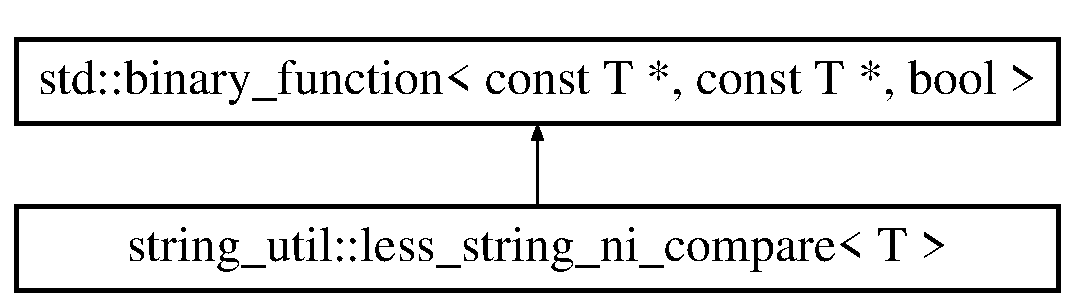
\includegraphics[height=2.000000cm]{classstring__util_1_1less__string__ni__compare}
\end{center}
\end{figure}
\subsection*{Public Member Functions}
\begin{DoxyCompactItemize}
\item 
{\bfseries less\+\_\+string\+\_\+ni\+\_\+compare} (size\+\_\+t comparison\+\_\+size)\label{classstring__util_1_1less__string__ni__compare_aec49bc79089ab2e54ff4752bbbabe6bf}

\item 
bool {\bfseries operator()} (const T $\ast$a\+\_\+, const T $\ast$b\+\_\+) const \label{classstring__util_1_1less__string__ni__compare_a6050f7d7b4998343cc5c46dca8b28bcc}

\end{DoxyCompactItemize}


The documentation for this class was generated from the following file\+:\begin{DoxyCompactItemize}
\item 
string\+\_\+util.\+h\end{DoxyCompactItemize}

\section{stemming\+:\+:no\+\_\+op\+\_\+stem$<$ string\+\_\+typeT $>$ Class Template Reference}
\label{classstemming_1_1no__op__stem}\index{stemming\+::no\+\_\+op\+\_\+stem$<$ string\+\_\+type\+T $>$@{stemming\+::no\+\_\+op\+\_\+stem$<$ string\+\_\+type\+T $>$}}
\subsection*{Public Member Functions}
\begin{DoxyCompactItemize}
\item 
void {\bf operator()} (const string\+\_\+typeT \&) const \label{classstemming_1_1no__op__stem_a5e95ea3afb739e7bea6b14a3e9150c89}

\begin{DoxyCompactList}\small\item\em No-\/op stemming of declared string type. \end{DoxyCompactList}\item 
{\footnotesize template$<$typename T $>$ }\\void {\bf operator()} (const T \&) const \label{classstemming_1_1no__op__stem_a8109dda5e97b7c138f9aa9ec9ea4ee9f}

\begin{DoxyCompactList}\small\item\em No-\/op stemming of flexible string type. \end{DoxyCompactList}\end{DoxyCompactItemize}


The documentation for this class was generated from the following file\+:\begin{DoxyCompactItemize}
\item 
/home/coder/\+C\+S\+E2341-\/17\+S-\/\+Lose-\/lose-\/situation/\+F\+Project/stemming.\+h\end{DoxyCompactItemize}

\section{Query\+Engine Class Reference}
\label{class_query_engine}\index{Query\+Engine@{Query\+Engine}}


The \doxyref{Query\+Engine}{p.}{class_query_engine} uses the inverted file index and searches it given a properly formatted Boolean query. It also ranks the results using tf/idf statistics.  




{\ttfamily \#include $<$queryengine.\+h$>$}

\subsection*{Public Member Functions}
\begin{DoxyCompactItemize}
\item 
{\bf Query\+Engine} ({\bf Index\+Handler} $\ast$, {\bf Document\+Parser} $\ast$)
\begin{DoxyCompactList}\small\item\em The \doxyref{Query\+Engine}{p.}{class_query_engine} uses the inverted file index and searches it given a properly formatted Boolean query. It also ranks the results using tf/idf statistics. \end{DoxyCompactList}\item 
vector$<$ {\bf document} $>$ {\bf query\+Search} (string query)
\begin{DoxyCompactList}\small\item\em \doxyref{Query\+Engine\+::query\+Search}{p.}{class_query_engine_aea1c3b1b81ab4755bb9450c73080ba58} This searches the inverted index file for a given boolean query. It calls the search method to earch for the words and returning the proper results based on whether a union, intersection or difference was required. \end{DoxyCompactList}\item 
vector$<$ {\bf document} $>$ {\bf search} (string word)
\begin{DoxyCompactList}\small\item\em \doxyref{Query\+Engine\+::search}{p.}{class_query_engine_a1a9e0cf429284793b690db04de09fd5f} This searches the inverted index file for a word, returning the results. \end{DoxyCompactList}\item 
vector$<$ {\bf document} $>$ {\bf get\+Intersection} (vector$<$ {\bf document} $>$ l, vector$<$ {\bf document} $>$ r)
\begin{DoxyCompactList}\small\item\em \doxyref{Query\+Engine\+::get\+Intersection}{p.}{class_query_engine_a5acd0880e616f8a0c4e126294fe516b8} This returns the intersection of two queries. \end{DoxyCompactList}\item 
vector$<$ {\bf document} $>$ {\bf get\+Union} (vector$<$ {\bf document} $>$ l, vector$<$ {\bf document} $>$ r)
\begin{DoxyCompactList}\small\item\em \doxyref{Query\+Engine\+::get\+Union}{p.}{class_query_engine_aee8574303264380c75ef2e02b0f76acf} This returns the union of two queries. \end{DoxyCompactList}\item 
vector$<$ {\bf document} $>$ {\bf get\+Difference} (vector$<$ {\bf document} $>$ r, vector$<$ {\bf document} $>$ l)
\begin{DoxyCompactList}\small\item\em \doxyref{Query\+Engine\+::get\+Difference}{p.}{class_query_engine_a57ef6547912ba509e2589b7b6cfe0d93} This returns the difference of two queries. \end{DoxyCompactList}\item 
void {\bf find\+T\+D\+I\+Fs} (vector$<$ {\bf document} $>$ \&currdocs)
\begin{DoxyCompactList}\small\item\em \doxyref{Query\+Engine\+::find\+T\+D\+I\+Fs}{p.}{class_query_engine_a8f580bd2a38cc08c68a2845f380d9547} This caculates the tf/idf values of the query results. \end{DoxyCompactList}\item 
void {\bf relevency\+Sort} (vector$<$ {\bf document} $>$ \&currdocs)
\begin{DoxyCompactList}\small\item\em \doxyref{Query\+Engine\+::relevency\+Sort}{p.}{class_query_engine_a11f70f58daaaa7dee67e52cc415bd13f} This sorts the vector$<$document$>$ by tf/idf value. \end{DoxyCompactList}\end{DoxyCompactItemize}
\subsection*{Public Attributes}
\begin{DoxyCompactItemize}
\item 
int {\bfseries file\+Size} =0\label{class_query_engine_a562077633097b8ccc4324df971ee23db}

\end{DoxyCompactItemize}


\subsection{Detailed Description}
The \doxyref{Query\+Engine}{p.}{class_query_engine} uses the inverted file index and searches it given a properly formatted Boolean query. It also ranks the results using tf/idf statistics. 

C\+SE 2341 Query\+Engine.\+h \begin{DoxyAuthor}{Author}
Aviraj Shina (owner) 
\end{DoxyAuthor}
\begin{DoxyVersion}{Version}
1.\+0 05/07/17 The \doxyref{Query\+Engine}{p.}{class_query_engine} class 
\end{DoxyVersion}


\subsection{Constructor \& Destructor Documentation}
\index{Query\+Engine@{Query\+Engine}!Query\+Engine@{Query\+Engine}}
\index{Query\+Engine@{Query\+Engine}!Query\+Engine@{Query\+Engine}}
\subsubsection[{Query\+Engine(\+Index\+Handler $\ast$, Document\+Parser $\ast$)}]{\setlength{\rightskip}{0pt plus 5cm}Query\+Engine\+::\+Query\+Engine (
\begin{DoxyParamCaption}
\item[{{\bf Index\+Handler} $\ast$}]{i, }
\item[{{\bf Document\+Parser} $\ast$}]{d}
\end{DoxyParamCaption}
)}\label{class_query_engine_a4f10c7d88f75039ac139209ad60c4867}


The \doxyref{Query\+Engine}{p.}{class_query_engine} uses the inverted file index and searches it given a properly formatted Boolean query. It also ranks the results using tf/idf statistics. 

C\+SE 2341 Query\+Engine.\+h \begin{DoxyAuthor}{Author}
Aviraj Shina (owner) 
\end{DoxyAuthor}
\begin{DoxyVersion}{Version}
1.\+0 05/07/17 \doxyref{Query\+Engine\+::\+Query\+Engine}{p.}{class_query_engine_a4f10c7d88f75039ac139209ad60c4867} The constructor for the query engine. 
\end{DoxyVersion}

\begin{DoxyParams}{Parameters}
{\em i} & The index handler object. \\
\hline
{\em d} & The documpen parser object. \\
\hline
\end{DoxyParams}


\subsection{Member Function Documentation}
\index{Query\+Engine@{Query\+Engine}!find\+T\+D\+I\+Fs@{find\+T\+D\+I\+Fs}}
\index{find\+T\+D\+I\+Fs@{find\+T\+D\+I\+Fs}!Query\+Engine@{Query\+Engine}}
\subsubsection[{find\+T\+D\+I\+Fs(vector$<$ document $>$ \&currdocs)}]{\setlength{\rightskip}{0pt plus 5cm}void Query\+Engine\+::find\+T\+D\+I\+Fs (
\begin{DoxyParamCaption}
\item[{vector$<$ {\bf document} $>$ \&}]{currdocs}
\end{DoxyParamCaption}
)}\label{class_query_engine_a8f580bd2a38cc08c68a2845f380d9547}


\doxyref{Query\+Engine\+::find\+T\+D\+I\+Fs}{p.}{class_query_engine_a8f580bd2a38cc08c68a2845f380d9547} This caculates the tf/idf values of the query results. 


\begin{DoxyParams}{Parameters}
{\em currdocs} & The vector$<$document$>$ to caculate the tf/idf for. \\
\hline
\end{DoxyParams}
\index{Query\+Engine@{Query\+Engine}!get\+Difference@{get\+Difference}}
\index{get\+Difference@{get\+Difference}!Query\+Engine@{Query\+Engine}}
\subsubsection[{get\+Difference(vector$<$ document $>$ r, vector$<$ document $>$ l)}]{\setlength{\rightskip}{0pt plus 5cm}vector$<$ {\bf document} $>$ Query\+Engine\+::get\+Difference (
\begin{DoxyParamCaption}
\item[{vector$<$ {\bf document} $>$}]{r, }
\item[{vector$<$ {\bf document} $>$}]{l}
\end{DoxyParamCaption}
)}\label{class_query_engine_a57ef6547912ba509e2589b7b6cfe0d93}


\doxyref{Query\+Engine\+::get\+Difference}{p.}{class_query_engine_a57ef6547912ba509e2589b7b6cfe0d93} This returns the difference of two queries. 


\begin{DoxyParams}{Parameters}
{\em l} & The vector$<$document$>$ of the first query. \\
\hline
{\em r} & The vector$<$document$>$ of the secnd query. \\
\hline
\end{DoxyParams}
\begin{DoxyReturn}{Returns}
vector$<$document$>$ The difference of the first and second query. 
\end{DoxyReturn}
\index{Query\+Engine@{Query\+Engine}!get\+Intersection@{get\+Intersection}}
\index{get\+Intersection@{get\+Intersection}!Query\+Engine@{Query\+Engine}}
\subsubsection[{get\+Intersection(vector$<$ document $>$ l, vector$<$ document $>$ r)}]{\setlength{\rightskip}{0pt plus 5cm}vector$<$ {\bf document} $>$ Query\+Engine\+::get\+Intersection (
\begin{DoxyParamCaption}
\item[{vector$<$ {\bf document} $>$}]{l, }
\item[{vector$<$ {\bf document} $>$}]{r}
\end{DoxyParamCaption}
)}\label{class_query_engine_a5acd0880e616f8a0c4e126294fe516b8}


\doxyref{Query\+Engine\+::get\+Intersection}{p.}{class_query_engine_a5acd0880e616f8a0c4e126294fe516b8} This returns the intersection of two queries. 


\begin{DoxyParams}{Parameters}
{\em l} & The vector$<$document$>$ of the first query. \\
\hline
{\em r} & The vector$<$document$>$ of the secnd query. \\
\hline
\end{DoxyParams}
\begin{DoxyReturn}{Returns}
vector$<$document$>$ The intersection of the first and second query. 
\end{DoxyReturn}
\index{Query\+Engine@{Query\+Engine}!get\+Union@{get\+Union}}
\index{get\+Union@{get\+Union}!Query\+Engine@{Query\+Engine}}
\subsubsection[{get\+Union(vector$<$ document $>$ l, vector$<$ document $>$ r)}]{\setlength{\rightskip}{0pt plus 5cm}vector$<$ {\bf document} $>$ Query\+Engine\+::get\+Union (
\begin{DoxyParamCaption}
\item[{vector$<$ {\bf document} $>$}]{l, }
\item[{vector$<$ {\bf document} $>$}]{r}
\end{DoxyParamCaption}
)}\label{class_query_engine_aee8574303264380c75ef2e02b0f76acf}


\doxyref{Query\+Engine\+::get\+Union}{p.}{class_query_engine_aee8574303264380c75ef2e02b0f76acf} This returns the union of two queries. 


\begin{DoxyParams}{Parameters}
{\em l} & The vector$<$document$>$ of the first query. \\
\hline
{\em r} & The vector$<$document$>$ of the secnd query. \\
\hline
\end{DoxyParams}
\begin{DoxyReturn}{Returns}
vector$<$document$>$ The union of the first and second query. 
\end{DoxyReturn}
\index{Query\+Engine@{Query\+Engine}!query\+Search@{query\+Search}}
\index{query\+Search@{query\+Search}!Query\+Engine@{Query\+Engine}}
\subsubsection[{query\+Search(string query)}]{\setlength{\rightskip}{0pt plus 5cm}vector$<$ {\bf document} $>$ Query\+Engine\+::query\+Search (
\begin{DoxyParamCaption}
\item[{string}]{query}
\end{DoxyParamCaption}
)}\label{class_query_engine_aea1c3b1b81ab4755bb9450c73080ba58}


\doxyref{Query\+Engine\+::query\+Search}{p.}{class_query_engine_aea1c3b1b81ab4755bb9450c73080ba58} This searches the inverted index file for a given boolean query. It calls the search method to earch for the words and returning the proper results based on whether a union, intersection or difference was required. 


\begin{DoxyParams}{Parameters}
{\em query} & The query to search for. \\
\hline
\end{DoxyParams}
\begin{DoxyReturn}{Returns}
vector$<$document$>$ A vector of document objects containing the results of the search sorted by tf/idf values. 
\end{DoxyReturn}
\index{Query\+Engine@{Query\+Engine}!relevency\+Sort@{relevency\+Sort}}
\index{relevency\+Sort@{relevency\+Sort}!Query\+Engine@{Query\+Engine}}
\subsubsection[{relevency\+Sort(vector$<$ document $>$ \&currdocs)}]{\setlength{\rightskip}{0pt plus 5cm}void Query\+Engine\+::relevency\+Sort (
\begin{DoxyParamCaption}
\item[{vector$<$ {\bf document} $>$ \&}]{currdocs}
\end{DoxyParamCaption}
)}\label{class_query_engine_a11f70f58daaaa7dee67e52cc415bd13f}


\doxyref{Query\+Engine\+::relevency\+Sort}{p.}{class_query_engine_a11f70f58daaaa7dee67e52cc415bd13f} This sorts the vector$<$document$>$ by tf/idf value. 


\begin{DoxyParams}{Parameters}
{\em currdocs} & The vector$<$document$>$ to be sorted. \\
\hline
\end{DoxyParams}
\index{Query\+Engine@{Query\+Engine}!search@{search}}
\index{search@{search}!Query\+Engine@{Query\+Engine}}
\subsubsection[{search(string word)}]{\setlength{\rightskip}{0pt plus 5cm}vector$<$ {\bf document} $>$ Query\+Engine\+::search (
\begin{DoxyParamCaption}
\item[{string}]{word}
\end{DoxyParamCaption}
)}\label{class_query_engine_a1a9e0cf429284793b690db04de09fd5f}


\doxyref{Query\+Engine\+::search}{p.}{class_query_engine_a1a9e0cf429284793b690db04de09fd5f} This searches the inverted index file for a word, returning the results. 


\begin{DoxyParams}{Parameters}
{\em word} & The word to search for. \\
\hline
\end{DoxyParams}
\begin{DoxyReturn}{Returns}
vector$<$document$>$ A vector of document objects containing the results of the search. 
\end{DoxyReturn}


The documentation for this class was generated from the following files\+:\begin{DoxyCompactItemize}
\item 
/home/coder/\+C\+S\+E2341-\/17\+S-\/\+Lose-\/lose-\/situation/\+F\+Project/queryengine.\+h\item 
/home/coder/\+C\+S\+E2341-\/17\+S-\/\+Lose-\/lose-\/situation/\+F\+Project/queryengine.\+cpp\end{DoxyCompactItemize}

\section{raw\+Output\+Extractor Class Reference}
\label{classraw_output_extractor}\index{raw\+Output\+Extractor@{raw\+Output\+Extractor}}


{\ttfamily \#include $<$rawoutputextractor.\+h$>$}

\subsection*{Public Member Functions}
\begin{DoxyCompactItemize}
\item 
{\bfseries raw\+Output\+Extractor} ({\bf Index\+Handler} $\ast$, {\bf indexextractor} $\ast$)\label{classraw_output_extractor_a9f1429b521b00d304082bb6b6e7aa810}

\item 
int {\bfseries get\+Total\+Pages} ()\label{classraw_output_extractor_a306ee3750845f8343c312524ab56119f}

\item 
string {\bfseries get\+Doc\+Name} ()\label{classraw_output_extractor_aaa6eefc03308e4ab23e5a07fd14ffc94}

\item 
int {\bfseries get\+Word\+Count} ()\label{classraw_output_extractor_a96366fc0b002b56285146c0a813ad76f}

\item 
void {\bfseries Init} (const char $\ast$psz\+Input)\label{classraw_output_extractor_a085aa59c775749e1f56363e8c195f3ef}

\end{DoxyCompactItemize}
\subsection*{Public Attributes}
\begin{DoxyCompactItemize}
\item 
{\bf Index\+Handler} $\ast$ {\bfseries ih}\label{classraw_output_extractor_ad067d96f81f783c6f5bc20227806250b}

\item 
{\bf indexextractor} $\ast$ {\bfseries ie}\label{classraw_output_extractor_a60443cbf3cec7845e65acb58fefe369e}

\item 
string {\bfseries mm}\label{classraw_output_extractor_a2423c51cd2139ea3da4239b620a3e5ab}

\item 
vector$<$ string $>$ {\bfseries a}\label{classraw_output_extractor_a7466d30c2340396fcde7a185e4405e26}

\item 
int {\bfseries word\+Count} =0\label{classraw_output_extractor_a44ba737833045854b190a30fab86f8bd}

\item 
string {\bfseries docs\+Name}\label{classraw_output_extractor_a10e7d598053ca6ffaf7f053eb8f39127}

\end{DoxyCompactItemize}


\subsection{Detailed Description}
This class uses the Po\+Do\+Fo lib to parse a P\+DF file and to write all text it finds in this P\+DF document to stdout. 

The documentation for this class was generated from the following files\+:\begin{DoxyCompactItemize}
\item 
rawoutputextractor.\+h\item 
rawoutputextractor.\+cpp\end{DoxyCompactItemize}

\section{Search\+Engine Class Reference}
\label{class_search_engine}\index{Search\+Engine@{Search\+Engine}}


The \doxyref{Search\+Engine}{p.}{class_search_engine} class.  




{\ttfamily \#include $<$searchengine.\+h$>$}

\subsection*{Public Member Functions}
\begin{DoxyCompactItemize}
\item 
{\bfseries Search\+Engine} (string docpath, char)\label{class_search_engine_a96042d7c914e9dec875f9f34efd42746}

\item 
{\bf Search\+Engine} ()
\begin{DoxyCompactList}\small\item\em The \doxyref{Search\+Engine}{p.}{class_search_engine} class uses the various class to create a P\+DF Search Engine. The class makes use of the \doxyref{Document\+Parser}{p.}{class_document_parser}, \doxyref{Index\+Handler}{p.}{class_index_handler}, and Query\+Engie class to perform all of the various tasks of the Mantience mode and Query mode of the user interface. \end{DoxyCompactList}\item 
vector$<$ {\bf document} $>$ {\bf display\+\_\+search\+\_\+results} (string word)
\begin{DoxyCompactList}\small\item\em \doxyref{Search\+Engine\+::display\+\_\+search\+\_\+results}{p.}{class_search_engine_a28b5caaf6c40264037ffab938c0a6916} This searches the inverted file index for a query and displays the results. \end{DoxyCompactList}\item 
void {\bfseries relevency\+Sort} (vector$<$ {\bf document} $>$ \&)\label{class_search_engine_abf44270499162aeb6b78ad9f72c89825}

\item 
void {\bf write\+Index} ()\label{class_search_engine_ad480df2432da22ce6556ada835112a4b}

\begin{DoxyCompactList}\small\item\em \doxyref{Search\+Engine\+::write\+Index}{p.}{class_search_engine_ad480df2432da22ce6556ada835112a4b} This writes the index from the appropriate data structure and into the inverted file index. \end{DoxyCompactList}\item 
void {\bf read\+Index} ()\label{class_search_engine_aefc6f13183bc05854205ca0dd1f2e22e}

\begin{DoxyCompactList}\small\item\em \doxyref{Search\+Engine\+::read\+Index}{p.}{class_search_engine_aefc6f13183bc05854205ca0dd1f2e22e} This reads the index from the inverted index file and into the appropriate data structure. \end{DoxyCompactList}\item 
void {\bf clear\+Index} ()\label{class_search_engine_a543e75d77f79c981b0c85bf3e6c4aa32}

\begin{DoxyCompactList}\small\item\em \doxyref{Search\+Engine\+::clear\+Index}{p.}{class_search_engine_a543e75d77f79c981b0c85bf3e6c4aa32} This clears the inverted file index (.txt file). \end{DoxyCompactList}\item 
int {\bf get\+Total\+Pages} ()
\begin{DoxyCompactList}\small\item\em \doxyref{Search\+Engine\+::get\+Total\+Pages}{p.}{class_search_engine_a213e139ff06e4a786eb0d4291ab36b3a} Returns the total page count. \end{DoxyCompactList}\item 
int {\bf num\+Words\+Indexed} ()
\begin{DoxyCompactList}\small\item\em \doxyref{Search\+Engine\+::num\+Words\+Indexed}{p.}{class_search_engine_aec2f16d453e857875e62777117b173a3} Returns the total indexed word count. \end{DoxyCompactList}\item 
vector$<$ {\bf document} $>$ {\bf topfifty} ()
\begin{DoxyCompactList}\small\item\em \doxyref{Search\+Engine\+::topfifty}{p.}{class_search_engine_a6e4fb46ec3e35b4fcd3e479b21398983} Returns the top fifty most common words. \end{DoxyCompactList}\item 
bool {\bf add\+Documents\+To\+Index} (string docpath)
\begin{DoxyCompactList}\small\item\em \doxyref{Search\+Engine\+::add\+Documents\+To\+Index}{p.}{class_search_engine_ac34ccd88ddb26e15843036a63f80ca22} Allows the user to choose between using a Hash table or A\+V\+L\+Tree to create the inverted index file. This also initalizes the \doxyref{Index\+Handler}{p.}{class_index_handler}, Documentparser, and \doxyref{Query\+Engine}{p.}{class_query_engine} objects to allow the Search Engine access to their functions. It also updtes the tf/idf, inverted file index, page count, word count, and top fifty words. \end{DoxyCompactList}\item 
void {\bf choose\+Structure} (char type)
\begin{DoxyCompactList}\small\item\em \doxyref{Search\+Engine\+::choose\+Structure}{p.}{class_search_engine_ab1b68eb5a1887426b044f041546cbbb2} Allows the user to choose between using a Hash table or A\+V\+L\+Tree to create the inverted index file. This also initalizes the \doxyref{Index\+Handler}{p.}{class_index_handler}, Documentparser, and \doxyref{Query\+Engine}{p.}{class_query_engine} objects to allow the Search Engine access to their functions. It also updtes the tf/idf, inverted file index, page count, word count, and top fifty words. \end{DoxyCompactList}\item 
void {\bfseries find\+T\+D\+I\+Fs} (vector$<$ {\bf document} $>$ \&currdocs)\label{class_search_engine_a3d873d763983aff96bfa5b53a5ce1857}

\item 
int {\bf read\+Total\+Pages} ()
\begin{DoxyCompactList}\small\item\em \doxyref{Search\+Engine\+::read\+Total\+Pages}{p.}{class_search_engine_aa5eeb7c14f04c71458626a4e42fb7f90} This outputs the total number of pages stored from the P\+D\+Fs on the inverted index. \end{DoxyCompactList}\item 
void {\bf clear\+Total\+Pages} ()\label{class_search_engine_a32cc85f13141666446a3970dccbf2b3f}

\begin{DoxyCompactList}\small\item\em \doxyref{Search\+Engine\+::clear\+Total\+Pages}{p.}{class_search_engine_a32cc85f13141666446a3970dccbf2b3f} This clears the total number of pages .txt file. \end{DoxyCompactList}\item 
void {\bf clear\+Word\+Txt} ()\label{class_search_engine_a7cbf38d7d2d78b8f85fcb722df5d509f}

\begin{DoxyCompactList}\small\item\em \doxyref{Search\+Engine\+::clear\+Word\+Txt}{p.}{class_search_engine_a7cbf38d7d2d78b8f85fcb722df5d509f} This clears the total indexed word count .txt file. \end{DoxyCompactList}\item 
void {\bf clear} ()\label{class_search_engine_a0fff04096cc03d5812306d35621556a0}

\begin{DoxyCompactList}\small\item\em \doxyref{Search\+Engine\+::clear}{p.}{class_search_engine_a0fff04096cc03d5812306d35621556a0} Allows the user to clear all of the stored data. It cleares the inverted file index, the total page count, the total indexed word count, the file paths, the bookmarks and the search history. \end{DoxyCompactList}\item 
bool {\bf display\+Raw\+File} (string file\+Path)
\begin{DoxyCompactList}\small\item\em \doxyref{Search\+Engine\+::display\+Raw\+File}{p.}{class_search_engine_ad995e4339f832125cd4de230bbf4343f} This dispalys the raw text of a requested P\+DF. \end{DoxyCompactList}\item 
void {\bf display\+Top50} ()\label{class_search_engine_a7afe7195e04733c109e8b3cd3d38c7be}

\begin{DoxyCompactList}\small\item\em \doxyref{Search\+Engine\+::display\+Top50}{p.}{class_search_engine_a7afe7195e04733c109e8b3cd3d38c7be} This displays the top fifty words from the P\+D\+Fs on the inverted index. \end{DoxyCompactList}\item 
void {\bf write\+File\+Path\+To\+T\+X\+T\+File} ()\label{class_search_engine_ab7e13d869a81e670969fc6f081340692}

\begin{DoxyCompactList}\small\item\em \doxyref{Search\+Engine\+::write\+File\+Path\+To\+T\+X\+T\+File}{p.}{class_search_engine_ab7e13d869a81e670969fc6f081340692} This writes the file paths to a text file allowing the path to be stored. \end{DoxyCompactList}\item 
vector$<$ string $>$ {\bf read\+File\+Path\+From\+T\+X\+T\+File} ()
\begin{DoxyCompactList}\small\item\em \doxyref{Search\+Engine\+::read\+File\+Path\+From\+T\+X\+T\+File}{p.}{class_search_engine_a010df9478350578057cf319fad1f6eea} This reads the file paths from the .txt file of file paths. \end{DoxyCompactList}\item 
void {\bf clear\+File\+Path} ()\label{class_search_engine_a898495849f799fdde2d626980e00882c}

\begin{DoxyCompactList}\small\item\em \doxyref{Search\+Engine\+::clear\+File\+Path}{p.}{class_search_engine_a898495849f799fdde2d626980e00882c} This clears the file path .txt file. \end{DoxyCompactList}\item 
void {\bfseries write\+Bookmark} (string book, string query)\label{class_search_engine_ac6a8ee08a20a31f6ba06fb1a85e695ad}

\item 
void {\bf read\+Bookmarks} ()\label{class_search_engine_ae5ad9234b0e6c8ebb408bb01693b9f33}

\begin{DoxyCompactList}\small\item\em \doxyref{Search\+Engine\+::read\+Bookmarks}{p.}{class_search_engine_ae5ad9234b0e6c8ebb408bb01693b9f33} This reads the bookmarks from the .txt file and adds them to the bookmark vector. \end{DoxyCompactList}\item 
void {\bf add\+Bookmark} (string book, string query)
\begin{DoxyCompactList}\small\item\em \doxyref{Search\+Engine\+::add\+Bookmark}{p.}{class_search_engine_afe7ea87d4ab4ff654d38b71624d12312} This adds bookmarks to the .txt file. \end{DoxyCompactList}\item 
void {\bf add\+To\+History} (string query)
\begin{DoxyCompactList}\small\item\em \doxyref{Search\+Engine\+::add\+To\+History}{p.}{class_search_engine_a1b8486fd4b7e4169e8a9dc61dab4346b} This adds the query to the search history. \end{DoxyCompactList}\item 
void {\bf clear\+History} ()\label{class_search_engine_a5ddd80c981473501dab71fa019356c46}

\begin{DoxyCompactList}\small\item\em \doxyref{Search\+Engine\+::clear\+History}{p.}{class_search_engine_a5ddd80c981473501dab71fa019356c46} This clears the history .txt file. \end{DoxyCompactList}\item 
void {\bf display\+History} ()\label{class_search_engine_a1c690004902e31c701f584fdbdec5438}

\begin{DoxyCompactList}\small\item\em \doxyref{Search\+Engine\+::display\+History}{p.}{class_search_engine_a1c690004902e31c701f584fdbdec5438} This displays the search history. \end{DoxyCompactList}\item 
void {\bf clear\+Bookmarks} ()\label{class_search_engine_addcad78e40a60301848ceb89426d64d3}

\begin{DoxyCompactList}\small\item\em Search\+Engine\+::clear\+Bookmarks\+This clears the bookmarks .txt file. \end{DoxyCompactList}\item 
vector$<$ {\bf bookmark} $>$ {\bf display\+Bookmarks} ()
\begin{DoxyCompactList}\small\item\em \doxyref{Search\+Engine\+::display\+Bookmarks}{p.}{class_search_engine_ab461f4ce41e02d2405ce8fad949a49bb} This displays the bookmarks. \end{DoxyCompactList}\end{DoxyCompactItemize}
\subsection*{Public Attributes}
\begin{DoxyCompactItemize}
\item 
int {\bfseries total\+Pages} =0\label{class_search_engine_a833ba7e860c954284b64a83e1e3556d8}

\end{DoxyCompactItemize}


\subsection{Detailed Description}
The \doxyref{Search\+Engine}{p.}{class_search_engine} class. 

\subsection{Constructor \& Destructor Documentation}
\index{Search\+Engine@{Search\+Engine}!Search\+Engine@{Search\+Engine}}
\index{Search\+Engine@{Search\+Engine}!Search\+Engine@{Search\+Engine}}
\subsubsection[{Search\+Engine()}]{\setlength{\rightskip}{0pt plus 5cm}Search\+Engine\+::\+Search\+Engine (
\begin{DoxyParamCaption}
{}
\end{DoxyParamCaption}
)}\label{class_search_engine_ab129d2c96c29c6dcf4a28abbe4168f6c}


The \doxyref{Search\+Engine}{p.}{class_search_engine} class uses the various class to create a P\+DF Search Engine. The class makes use of the \doxyref{Document\+Parser}{p.}{class_document_parser}, \doxyref{Index\+Handler}{p.}{class_index_handler}, and Query\+Engie class to perform all of the various tasks of the Mantience mode and Query mode of the user interface. 

C\+SE 2341 Search\+Engine.\+cpp \begin{DoxyAuthor}{Author}
Aviraj Shina (owner) 

Patrick Yienger 
\end{DoxyAuthor}
\begin{DoxyVersion}{Version}
1.\+0 05/07/17 Search\+Engine\+::\+Search\+Engine The search engine constructor. 
\end{DoxyVersion}


\subsection{Member Function Documentation}
\index{Search\+Engine@{Search\+Engine}!add\+Bookmark@{add\+Bookmark}}
\index{add\+Bookmark@{add\+Bookmark}!Search\+Engine@{Search\+Engine}}
\subsubsection[{add\+Bookmark(string book, string query)}]{\setlength{\rightskip}{0pt plus 5cm}void Search\+Engine\+::add\+Bookmark (
\begin{DoxyParamCaption}
\item[{string}]{book, }
\item[{string}]{query}
\end{DoxyParamCaption}
)}\label{class_search_engine_afe7ea87d4ab4ff654d38b71624d12312}


\doxyref{Search\+Engine\+::add\+Bookmark}{p.}{class_search_engine_afe7ea87d4ab4ff654d38b71624d12312} This adds bookmarks to the .txt file. 


\begin{DoxyParams}{Parameters}
{\em book} & The bookmark to be added. \\
\hline
{\em query} & The query the bookmark was from. \\
\hline
\end{DoxyParams}
\index{Search\+Engine@{Search\+Engine}!add\+Documents\+To\+Index@{add\+Documents\+To\+Index}}
\index{add\+Documents\+To\+Index@{add\+Documents\+To\+Index}!Search\+Engine@{Search\+Engine}}
\subsubsection[{add\+Documents\+To\+Index(string docpath)}]{\setlength{\rightskip}{0pt plus 5cm}bool Search\+Engine\+::add\+Documents\+To\+Index (
\begin{DoxyParamCaption}
\item[{string}]{docpath}
\end{DoxyParamCaption}
)}\label{class_search_engine_ac34ccd88ddb26e15843036a63f80ca22}


\doxyref{Search\+Engine\+::add\+Documents\+To\+Index}{p.}{class_search_engine_ac34ccd88ddb26e15843036a63f80ca22} Allows the user to choose between using a Hash table or A\+V\+L\+Tree to create the inverted index file. This also initalizes the \doxyref{Index\+Handler}{p.}{class_index_handler}, Documentparser, and \doxyref{Query\+Engine}{p.}{class_query_engine} objects to allow the Search Engine access to their functions. It also updtes the tf/idf, inverted file index, page count, word count, and top fifty words. 


\begin{DoxyParams}{Parameters}
{\em type} & The user choice \\
\hline
\end{DoxyParams}
\begin{DoxyReturn}{Returns}
bool The flag for a sucessful text extract. 
\end{DoxyReturn}
\index{Search\+Engine@{Search\+Engine}!add\+To\+History@{add\+To\+History}}
\index{add\+To\+History@{add\+To\+History}!Search\+Engine@{Search\+Engine}}
\subsubsection[{add\+To\+History(string query)}]{\setlength{\rightskip}{0pt plus 5cm}void Search\+Engine\+::add\+To\+History (
\begin{DoxyParamCaption}
\item[{string}]{query}
\end{DoxyParamCaption}
)}\label{class_search_engine_a1b8486fd4b7e4169e8a9dc61dab4346b}


\doxyref{Search\+Engine\+::add\+To\+History}{p.}{class_search_engine_a1b8486fd4b7e4169e8a9dc61dab4346b} This adds the query to the search history. 


\begin{DoxyParams}{Parameters}
{\em query} & The query to be added. \\
\hline
\end{DoxyParams}
\index{Search\+Engine@{Search\+Engine}!choose\+Structure@{choose\+Structure}}
\index{choose\+Structure@{choose\+Structure}!Search\+Engine@{Search\+Engine}}
\subsubsection[{choose\+Structure(char type)}]{\setlength{\rightskip}{0pt plus 5cm}void Search\+Engine\+::choose\+Structure (
\begin{DoxyParamCaption}
\item[{char}]{type}
\end{DoxyParamCaption}
)}\label{class_search_engine_ab1b68eb5a1887426b044f041546cbbb2}


\doxyref{Search\+Engine\+::choose\+Structure}{p.}{class_search_engine_ab1b68eb5a1887426b044f041546cbbb2} Allows the user to choose between using a Hash table or A\+V\+L\+Tree to create the inverted index file. This also initalizes the \doxyref{Index\+Handler}{p.}{class_index_handler}, Documentparser, and \doxyref{Query\+Engine}{p.}{class_query_engine} objects to allow the Search Engine access to their functions. It also updtes the tf/idf, inverted file index, page count, word count, and top fifty words. 


\begin{DoxyParams}{Parameters}
{\em type} & The user choice \\
\hline
\end{DoxyParams}
\index{Search\+Engine@{Search\+Engine}!display\+\_\+search\+\_\+results@{display\+\_\+search\+\_\+results}}
\index{display\+\_\+search\+\_\+results@{display\+\_\+search\+\_\+results}!Search\+Engine@{Search\+Engine}}
\subsubsection[{display\+\_\+search\+\_\+results(string word)}]{\setlength{\rightskip}{0pt plus 5cm}vector$<$ {\bf document} $>$ Search\+Engine\+::display\+\_\+search\+\_\+results (
\begin{DoxyParamCaption}
\item[{string}]{word}
\end{DoxyParamCaption}
)}\label{class_search_engine_a28b5caaf6c40264037ffab938c0a6916}


\doxyref{Search\+Engine\+::display\+\_\+search\+\_\+results}{p.}{class_search_engine_a28b5caaf6c40264037ffab938c0a6916} This searches the inverted file index for a query and displays the results. 


\begin{DoxyParams}{Parameters}
{\em word} & The query to search for. \\
\hline
\end{DoxyParams}
\begin{DoxyReturn}{Returns}
vector$<$document$>$ The vector containing the document objects from the query search. 
\end{DoxyReturn}
\index{Search\+Engine@{Search\+Engine}!display\+Bookmarks@{display\+Bookmarks}}
\index{display\+Bookmarks@{display\+Bookmarks}!Search\+Engine@{Search\+Engine}}
\subsubsection[{display\+Bookmarks()}]{\setlength{\rightskip}{0pt plus 5cm}vector$<$ {\bf bookmark} $>$ Search\+Engine\+::display\+Bookmarks (
\begin{DoxyParamCaption}
{}
\end{DoxyParamCaption}
)}\label{class_search_engine_ab461f4ce41e02d2405ce8fad949a49bb}


\doxyref{Search\+Engine\+::display\+Bookmarks}{p.}{class_search_engine_ab461f4ce41e02d2405ce8fad949a49bb} This displays the bookmarks. 

\begin{DoxyReturn}{Returns}
vector$<$bookmarks$>$ The vector of bookmark objects that were displayed. 
\end{DoxyReturn}
\index{Search\+Engine@{Search\+Engine}!display\+Raw\+File@{display\+Raw\+File}}
\index{display\+Raw\+File@{display\+Raw\+File}!Search\+Engine@{Search\+Engine}}
\subsubsection[{display\+Raw\+File(string file\+Path)}]{\setlength{\rightskip}{0pt plus 5cm}bool Search\+Engine\+::display\+Raw\+File (
\begin{DoxyParamCaption}
\item[{string}]{file\+Path}
\end{DoxyParamCaption}
)}\label{class_search_engine_ad995e4339f832125cd4de230bbf4343f}


\doxyref{Search\+Engine\+::display\+Raw\+File}{p.}{class_search_engine_ad995e4339f832125cd4de230bbf4343f} This dispalys the raw text of a requested P\+DF. 


\begin{DoxyParams}{Parameters}
{\em file\+Path} & The path to the requested P\+DF \\
\hline
\end{DoxyParams}
\begin{DoxyReturn}{Returns}
bool The flag for a successful text extract. 
\end{DoxyReturn}
\index{Search\+Engine@{Search\+Engine}!get\+Total\+Pages@{get\+Total\+Pages}}
\index{get\+Total\+Pages@{get\+Total\+Pages}!Search\+Engine@{Search\+Engine}}
\subsubsection[{get\+Total\+Pages()}]{\setlength{\rightskip}{0pt plus 5cm}int Search\+Engine\+::get\+Total\+Pages (
\begin{DoxyParamCaption}
{}
\end{DoxyParamCaption}
)}\label{class_search_engine_a213e139ff06e4a786eb0d4291ab36b3a}


\doxyref{Search\+Engine\+::get\+Total\+Pages}{p.}{class_search_engine_a213e139ff06e4a786eb0d4291ab36b3a} Returns the total page count. 

\begin{DoxyReturn}{Returns}
pages The total page count. 
\end{DoxyReturn}
\index{Search\+Engine@{Search\+Engine}!num\+Words\+Indexed@{num\+Words\+Indexed}}
\index{num\+Words\+Indexed@{num\+Words\+Indexed}!Search\+Engine@{Search\+Engine}}
\subsubsection[{num\+Words\+Indexed()}]{\setlength{\rightskip}{0pt plus 5cm}int Search\+Engine\+::num\+Words\+Indexed (
\begin{DoxyParamCaption}
{}
\end{DoxyParamCaption}
)}\label{class_search_engine_aec2f16d453e857875e62777117b173a3}


\doxyref{Search\+Engine\+::num\+Words\+Indexed}{p.}{class_search_engine_aec2f16d453e857875e62777117b173a3} Returns the total indexed word count. 

\begin{DoxyReturn}{Returns}
total\+Words\+Indexed 
\end{DoxyReturn}
\index{Search\+Engine@{Search\+Engine}!read\+File\+Path\+From\+T\+X\+T\+File@{read\+File\+Path\+From\+T\+X\+T\+File}}
\index{read\+File\+Path\+From\+T\+X\+T\+File@{read\+File\+Path\+From\+T\+X\+T\+File}!Search\+Engine@{Search\+Engine}}
\subsubsection[{read\+File\+Path\+From\+T\+X\+T\+File()}]{\setlength{\rightskip}{0pt plus 5cm}vector$<$ string $>$ Search\+Engine\+::read\+File\+Path\+From\+T\+X\+T\+File (
\begin{DoxyParamCaption}
{}
\end{DoxyParamCaption}
)}\label{class_search_engine_a010df9478350578057cf319fad1f6eea}


\doxyref{Search\+Engine\+::read\+File\+Path\+From\+T\+X\+T\+File}{p.}{class_search_engine_a010df9478350578057cf319fad1f6eea} This reads the file paths from the .txt file of file paths. 

\begin{DoxyReturn}{Returns}
vector$<$string$>$ The vector of the file paths. 
\end{DoxyReturn}
\index{Search\+Engine@{Search\+Engine}!read\+Total\+Pages@{read\+Total\+Pages}}
\index{read\+Total\+Pages@{read\+Total\+Pages}!Search\+Engine@{Search\+Engine}}
\subsubsection[{read\+Total\+Pages()}]{\setlength{\rightskip}{0pt plus 5cm}int Search\+Engine\+::read\+Total\+Pages (
\begin{DoxyParamCaption}
{}
\end{DoxyParamCaption}
)}\label{class_search_engine_aa5eeb7c14f04c71458626a4e42fb7f90}


\doxyref{Search\+Engine\+::read\+Total\+Pages}{p.}{class_search_engine_aa5eeb7c14f04c71458626a4e42fb7f90} This outputs the total number of pages stored from the P\+D\+Fs on the inverted index. 

\begin{DoxyReturn}{Returns}
total\+Pages 
\end{DoxyReturn}
\index{Search\+Engine@{Search\+Engine}!topfifty@{topfifty}}
\index{topfifty@{topfifty}!Search\+Engine@{Search\+Engine}}
\subsubsection[{topfifty()}]{\setlength{\rightskip}{0pt plus 5cm}vector$<$ {\bf document} $>$ Search\+Engine\+::topfifty (
\begin{DoxyParamCaption}
{}
\end{DoxyParamCaption}
)}\label{class_search_engine_a6e4fb46ec3e35b4fcd3e479b21398983}


\doxyref{Search\+Engine\+::topfifty}{p.}{class_search_engine_a6e4fb46ec3e35b4fcd3e479b21398983} Returns the top fifty most common words. 

\begin{DoxyReturn}{Returns}
top50 The vector$<$document$>$ containing the top fifty words and their count. 
\end{DoxyReturn}


The documentation for this class was generated from the following files\+:\begin{DoxyCompactItemize}
\item 
searchengine.\+h\item 
searchengine.\+cpp\end{DoxyCompactItemize}

\section{stemming\+:\+:stem$<$ string\+\_\+typeT $>$ Class Template Reference}
\label{classstemming_1_1stem}\index{stemming\+::stem$<$ string\+\_\+type\+T $>$@{stemming\+::stem$<$ string\+\_\+type\+T $>$}}


The base class for language-\/specific stemmers.  




{\ttfamily \#include $<$stemming.\+h$>$}

Inheritance diagram for stemming\+:\+:stem$<$ string\+\_\+typeT $>$\+:\begin{figure}[H]
\begin{center}
\leavevmode
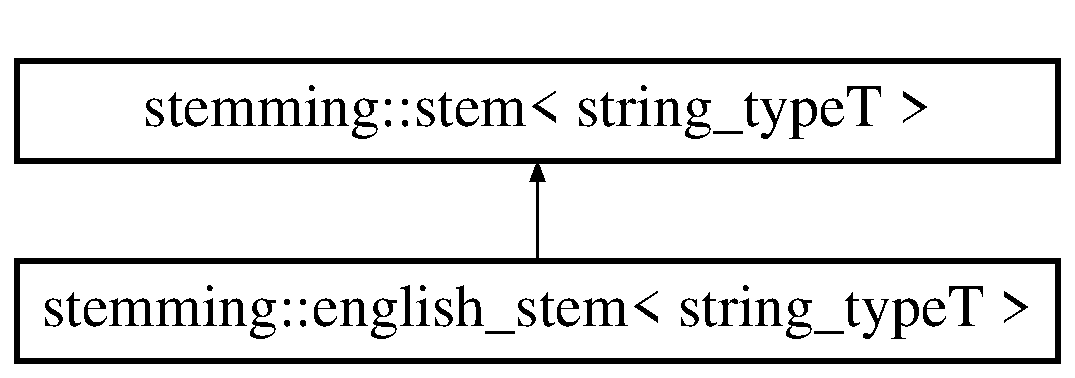
\includegraphics[height=2.000000cm]{classstemming_1_1stem}
\end{center}
\end{figure}
\subsection*{Protected Member Functions}
\begin{DoxyCompactItemize}
\item 
void {\bfseries find\+\_\+r1} (const string\+\_\+typeT \&text, const wchar\+\_\+t $\ast$vowel\+\_\+list)\label{classstemming_1_1stem_a364b7a76f683d5244715638069a4fa93}

\item 
void {\bfseries find\+\_\+r2} (const string\+\_\+typeT \&text, const wchar\+\_\+t $\ast$vowel\+\_\+list)\label{classstemming_1_1stem_ab381c0d6a6291c2c21515e9398e83085}

\item 
void {\bfseries find\+\_\+spanish\+\_\+rv} (const string\+\_\+typeT \&text, const wchar\+\_\+t $\ast$vowel\+\_\+list)\label{classstemming_1_1stem_ae6cb258098ba91462d421977b1eed8e7}

\item 
void {\bfseries find\+\_\+french\+\_\+rv} (const string\+\_\+typeT \&text, const wchar\+\_\+t $\ast$vowel\+\_\+list)\label{classstemming_1_1stem_a9626e49b982eda0d8ec3bb861d864b42}

\item 
void {\bfseries find\+\_\+russian\+\_\+rv} (const string\+\_\+typeT \&text, const wchar\+\_\+t $\ast$vowel\+\_\+list)\label{classstemming_1_1stem_a53dcfe6b18fe5b5882474f222190ef1b}

\item 
void {\bfseries update\+\_\+r\+\_\+sections} (const string\+\_\+typeT \&text)\label{classstemming_1_1stem_a9dcc3d89844ecd5c81eabf80936a0209}

\item 
bool {\bf is\+\_\+apostrophe} (const wchar\+\_\+t \&ch) const 
\item 
void {\bfseries trim\+\_\+western\+\_\+punctuation} (string\+\_\+typeT \&text) const \label{classstemming_1_1stem_a36818a956dd34c388fa9942ed46e28b4}

\item 
bool {\bf is\+\_\+suffix} (const string\+\_\+typeT \&text, const wchar\+\_\+t suffix1L, const wchar\+\_\+t suffix1U) const \label{classstemming_1_1stem_ac318ddd46a716673edf3678c47d3035c}

\begin{DoxyCompactList}\small\item\em is\+\_\+suffix for one character \end{DoxyCompactList}\item 
bool {\bf is\+\_\+suffix} (const string\+\_\+typeT \&text, const wchar\+\_\+t suffix1L, const wchar\+\_\+t suffix1U, const wchar\+\_\+t suffix2L, const wchar\+\_\+t suffix2U) const \label{classstemming_1_1stem_aad4dff424a3ae8a82dcfe6adac7c9d30}

\begin{DoxyCompactList}\small\item\em is\+\_\+suffix for two characters \end{DoxyCompactList}\item 
bool {\bf is\+\_\+suffix} (const string\+\_\+typeT \&text, const wchar\+\_\+t suffix1L, const wchar\+\_\+t suffix1U, const wchar\+\_\+t suffix2L, const wchar\+\_\+t suffix2U, const wchar\+\_\+t suffix3L, const wchar\+\_\+t suffix3U) const \label{classstemming_1_1stem_abbe6496d43b49dab0745e6d6b4e2831d}

\begin{DoxyCompactList}\small\item\em is\+\_\+suffix for three characters \end{DoxyCompactList}\item 
bool {\bf is\+\_\+suffix} (const string\+\_\+typeT \&text, const wchar\+\_\+t suffix1L, const wchar\+\_\+t suffix1U, const wchar\+\_\+t suffix2L, const wchar\+\_\+t suffix2U, const wchar\+\_\+t suffix3L, const wchar\+\_\+t suffix3U, const wchar\+\_\+t suffix4L, const wchar\+\_\+t suffix4U) const \label{classstemming_1_1stem_a694dd20e52adc89edadf120bf92a28ff}

\begin{DoxyCompactList}\small\item\em is\+\_\+suffix for four characters \end{DoxyCompactList}\item 
bool {\bf is\+\_\+suffix} (const string\+\_\+typeT \&text, const wchar\+\_\+t suffix1L, const wchar\+\_\+t suffix1U, const wchar\+\_\+t suffix2L, const wchar\+\_\+t suffix2U, const wchar\+\_\+t suffix3L, const wchar\+\_\+t suffix3U, const wchar\+\_\+t suffix4L, const wchar\+\_\+t suffix4U, const wchar\+\_\+t suffix5L, const wchar\+\_\+t suffix5U) const \label{classstemming_1_1stem_a001757aa7530b8acea05df8405def025}

\begin{DoxyCompactList}\small\item\em is\+\_\+suffix for five characters \end{DoxyCompactList}\item 
bool {\bf is\+\_\+suffix} (const string\+\_\+typeT \&text, const wchar\+\_\+t suffix1L, const wchar\+\_\+t suffix1U, const wchar\+\_\+t suffix2L, const wchar\+\_\+t suffix2U, const wchar\+\_\+t suffix3L, const wchar\+\_\+t suffix3U, const wchar\+\_\+t suffix4L, const wchar\+\_\+t suffix4U, const wchar\+\_\+t suffix5L, const wchar\+\_\+t suffix5U, const wchar\+\_\+t suffix6L, const wchar\+\_\+t suffix6U) const \label{classstemming_1_1stem_abe83f7592028b43f5cec9ce35ae1d9df}

\begin{DoxyCompactList}\small\item\em is\+\_\+suffix for six characters \end{DoxyCompactList}\item 
bool {\bf is\+\_\+suffix} (const string\+\_\+typeT \&text, const wchar\+\_\+t suffix1L, const wchar\+\_\+t suffix1U, const wchar\+\_\+t suffix2L, const wchar\+\_\+t suffix2U, const wchar\+\_\+t suffix3L, const wchar\+\_\+t suffix3U, const wchar\+\_\+t suffix4L, const wchar\+\_\+t suffix4U, const wchar\+\_\+t suffix5L, const wchar\+\_\+t suffix5U, const wchar\+\_\+t suffix6L, const wchar\+\_\+t suffix6U, const wchar\+\_\+t suffix7L, const wchar\+\_\+t suffix7U) const \label{classstemming_1_1stem_a79f18e256337d37054c80de470660a65}

\begin{DoxyCompactList}\small\item\em is\+\_\+suffix for seven characters \end{DoxyCompactList}\item 
bool {\bf is\+\_\+suffix} (const string\+\_\+typeT \&text, const wchar\+\_\+t suffix1L, const wchar\+\_\+t suffix1U, const wchar\+\_\+t suffix2L, const wchar\+\_\+t suffix2U, const wchar\+\_\+t suffix3L, const wchar\+\_\+t suffix3U, const wchar\+\_\+t suffix4L, const wchar\+\_\+t suffix4U, const wchar\+\_\+t suffix5L, const wchar\+\_\+t suffix5U, const wchar\+\_\+t suffix6L, const wchar\+\_\+t suffix6U, const wchar\+\_\+t suffix7L, const wchar\+\_\+t suffix7U, const wchar\+\_\+t suffix8L, const wchar\+\_\+t suffix8U) const \label{classstemming_1_1stem_aa18daf5b33d220d93dff22d6e591edd6}

\begin{DoxyCompactList}\small\item\em is\+\_\+suffix for eight characters \end{DoxyCompactList}\item 
bool {\bf is\+\_\+suffix} (const string\+\_\+typeT \&text, const wchar\+\_\+t suffix1L, const wchar\+\_\+t suffix1U, const wchar\+\_\+t suffix2L, const wchar\+\_\+t suffix2U, const wchar\+\_\+t suffix3L, const wchar\+\_\+t suffix3U, const wchar\+\_\+t suffix4L, const wchar\+\_\+t suffix4U, const wchar\+\_\+t suffix5L, const wchar\+\_\+t suffix5U, const wchar\+\_\+t suffix6L, const wchar\+\_\+t suffix6U, const wchar\+\_\+t suffix7L, const wchar\+\_\+t suffix7U, const wchar\+\_\+t suffix8L, const wchar\+\_\+t suffix8U, const wchar\+\_\+t suffix9L, const wchar\+\_\+t suffix9U) const \label{classstemming_1_1stem_ab905150e381f068c6b04eba851bb6263}

\begin{DoxyCompactList}\small\item\em is\+\_\+suffix for nine characters \end{DoxyCompactList}\item 
bool {\bf is\+\_\+partial\+\_\+suffix} (const string\+\_\+typeT \&text, const size\+\_\+t start\+\_\+index, const wchar\+\_\+t suffix1L, const wchar\+\_\+t suffix1U, const wchar\+\_\+t suffix2L, const wchar\+\_\+t suffix2U)\label{classstemming_1_1stem_a2ae63cf92bc4f4f40f0093e4842a235f}

\begin{DoxyCompactList}\small\item\em comparison for two characters \end{DoxyCompactList}\item 
bool {\bf is\+\_\+partial\+\_\+suffix} (const string\+\_\+typeT \&text, const size\+\_\+t start\+\_\+index, const wchar\+\_\+t suffix1L, const wchar\+\_\+t suffix1U, const wchar\+\_\+t suffix2L, const wchar\+\_\+t suffix2U, const wchar\+\_\+t suffix3L, const wchar\+\_\+t suffix3U)\label{classstemming_1_1stem_a728ea4e26737b04d04e02bea863f29e4}

\begin{DoxyCompactList}\small\item\em comparison for three characters \end{DoxyCompactList}\item 
bool {\bf is\+\_\+suffix\+\_\+in\+\_\+rv} (const string\+\_\+typeT \&text, const wchar\+\_\+t suffix1L, const wchar\+\_\+t suffix1U)
\begin{DoxyCompactList}\small\item\em RV suffix functions. \end{DoxyCompactList}\item 
bool {\bf is\+\_\+suffix\+\_\+in\+\_\+rv} (const string\+\_\+typeT \&text, const wchar\+\_\+t suffix1L, const wchar\+\_\+t suffix1U, const wchar\+\_\+t suffix2L, const wchar\+\_\+t suffix2U)\label{classstemming_1_1stem_a359356fbaafc3c7154d94fda6916ffa0}

\begin{DoxyCompactList}\small\item\em RV suffix comparison for two characters. \end{DoxyCompactList}\item 
bool {\bf is\+\_\+suffix\+\_\+in\+\_\+rv} (const string\+\_\+typeT \&text, const wchar\+\_\+t suffix1L, const wchar\+\_\+t suffix1U, const wchar\+\_\+t suffix2L, const wchar\+\_\+t suffix2U, const wchar\+\_\+t suffix3L, const wchar\+\_\+t suffix3U)\label{classstemming_1_1stem_a00fa5d00ff53320a437fe96a5bfa8f44}

\begin{DoxyCompactList}\small\item\em RV suffix comparison for three characters. \end{DoxyCompactList}\item 
bool {\bf is\+\_\+suffix\+\_\+in\+\_\+rv} (const string\+\_\+typeT \&text, const wchar\+\_\+t suffix1L, const wchar\+\_\+t suffix1U, const wchar\+\_\+t suffix2L, const wchar\+\_\+t suffix2U, const wchar\+\_\+t suffix3L, const wchar\+\_\+t suffix3U, const wchar\+\_\+t suffix4L, const wchar\+\_\+t suffix4U)\label{classstemming_1_1stem_acdaff4e73f7f3841beed04775b5d4f21}

\begin{DoxyCompactList}\small\item\em RV suffix comparison for four characters. \end{DoxyCompactList}\item 
bool {\bf is\+\_\+suffix\+\_\+in\+\_\+rv} (const string\+\_\+typeT \&text, const wchar\+\_\+t suffix1L, const wchar\+\_\+t suffix1U, const wchar\+\_\+t suffix2L, const wchar\+\_\+t suffix2U, const wchar\+\_\+t suffix3L, const wchar\+\_\+t suffix3U, const wchar\+\_\+t suffix4L, const wchar\+\_\+t suffix4U, const wchar\+\_\+t suffix5L, const wchar\+\_\+t suffix5U)\label{classstemming_1_1stem_a99ef9b0e80da18c39cc0206a666bd4b1}

\begin{DoxyCompactList}\small\item\em RV suffix comparison for five characters. \end{DoxyCompactList}\item 
bool {\bf is\+\_\+suffix\+\_\+in\+\_\+rv} (const string\+\_\+typeT \&text, const wchar\+\_\+t suffix1L, const wchar\+\_\+t suffix1U, const wchar\+\_\+t suffix2L, const wchar\+\_\+t suffix2U, const wchar\+\_\+t suffix3L, const wchar\+\_\+t suffix3U, const wchar\+\_\+t suffix4L, const wchar\+\_\+t suffix4U, const wchar\+\_\+t suffix5L, const wchar\+\_\+t suffix5U, const wchar\+\_\+t suffix6L, const wchar\+\_\+t suffix6U)\label{classstemming_1_1stem_a527b081fee02f191713a50dbc396f986}

\begin{DoxyCompactList}\small\item\em RV suffix comparison for six characters. \end{DoxyCompactList}\item 
bool {\bf is\+\_\+suffix\+\_\+in\+\_\+rv} (const string\+\_\+typeT \&text, const wchar\+\_\+t suffix1L, const wchar\+\_\+t suffix1U, const wchar\+\_\+t suffix2L, const wchar\+\_\+t suffix2U, const wchar\+\_\+t suffix3L, const wchar\+\_\+t suffix3U, const wchar\+\_\+t suffix4L, const wchar\+\_\+t suffix4U, const wchar\+\_\+t suffix5L, const wchar\+\_\+t suffix5U, const wchar\+\_\+t suffix6L, const wchar\+\_\+t suffix6U, const wchar\+\_\+t suffix7L, const wchar\+\_\+t suffix7U)\label{classstemming_1_1stem_abd6431b54fc5175c29809c627c44a587}

\begin{DoxyCompactList}\small\item\em RV suffix comparison for seven characters. \end{DoxyCompactList}\item 
bool {\bf is\+\_\+suffix\+\_\+in\+\_\+rv} (const string\+\_\+typeT \&text, const wchar\+\_\+t suffix1L, const wchar\+\_\+t suffix1U, const wchar\+\_\+t suffix2L, const wchar\+\_\+t suffix2U, const wchar\+\_\+t suffix3L, const wchar\+\_\+t suffix3U, const wchar\+\_\+t suffix4L, const wchar\+\_\+t suffix4U, const wchar\+\_\+t suffix5L, const wchar\+\_\+t suffix5U, const wchar\+\_\+t suffix6L, const wchar\+\_\+t suffix6U, const wchar\+\_\+t suffix7L, const wchar\+\_\+t suffix7U, const wchar\+\_\+t suffix8L, const wchar\+\_\+t suffix8U)\label{classstemming_1_1stem_a553b6ed34e6b03e2c1ca42ea2db08ba6}

\begin{DoxyCompactList}\small\item\em RV suffix comparison for eight characters. \end{DoxyCompactList}\item 
bool {\bf is\+\_\+suffix\+\_\+in\+\_\+r1} (const string\+\_\+typeT \&text, const wchar\+\_\+t suffix1L, const wchar\+\_\+t suffix1U)
\begin{DoxyCompactList}\small\item\em R1 suffix functions. \end{DoxyCompactList}\item 
bool {\bf is\+\_\+suffix\+\_\+in\+\_\+r1} (const string\+\_\+typeT \&text, const wchar\+\_\+t suffix1L, const wchar\+\_\+t suffix1U, const wchar\+\_\+t suffix2L, const wchar\+\_\+t suffix2U)\label{classstemming_1_1stem_ab8cb2e00b39091f74b1064e1f0314c6f}

\begin{DoxyCompactList}\small\item\em R1 suffix comparison for two characters. \end{DoxyCompactList}\item 
bool {\bf is\+\_\+suffix\+\_\+in\+\_\+r1} (const string\+\_\+typeT \&text, const wchar\+\_\+t suffix1L, const wchar\+\_\+t suffix1U, const wchar\+\_\+t suffix2L, const wchar\+\_\+t suffix2U, const wchar\+\_\+t suffix3L, const wchar\+\_\+t suffix3U)\label{classstemming_1_1stem_a1fe4a63adfa5d4f378a060352d52edc1}

\begin{DoxyCompactList}\small\item\em R1 suffix comparison for three characters. \end{DoxyCompactList}\item 
bool {\bf is\+\_\+suffix\+\_\+in\+\_\+r1} (const string\+\_\+typeT \&text, const wchar\+\_\+t suffix1L, const wchar\+\_\+t suffix1U, const wchar\+\_\+t suffix2L, const wchar\+\_\+t suffix2U, const wchar\+\_\+t suffix3L, const wchar\+\_\+t suffix3U, const wchar\+\_\+t suffix4L, const wchar\+\_\+t suffix4U)\label{classstemming_1_1stem_a3fef2f8916933fa1965928f8e43a1b58}

\begin{DoxyCompactList}\small\item\em R1 suffix comparison for four characters. \end{DoxyCompactList}\item 
bool {\bf is\+\_\+suffix\+\_\+in\+\_\+r1} (const string\+\_\+typeT \&text, const wchar\+\_\+t suffix1L, const wchar\+\_\+t suffix1U, const wchar\+\_\+t suffix2L, const wchar\+\_\+t suffix2U, const wchar\+\_\+t suffix3L, const wchar\+\_\+t suffix3U, const wchar\+\_\+t suffix4L, const wchar\+\_\+t suffix4U, const wchar\+\_\+t suffix5L, const wchar\+\_\+t suffix5U)\label{classstemming_1_1stem_a88f0e5e0cc055f013b6321215eb18ef3}

\begin{DoxyCompactList}\small\item\em R1 suffix comparison for five characters. \end{DoxyCompactList}\item 
bool {\bf is\+\_\+suffix\+\_\+in\+\_\+r1} (const string\+\_\+typeT \&text, const wchar\+\_\+t suffix1L, const wchar\+\_\+t suffix1U, const wchar\+\_\+t suffix2L, const wchar\+\_\+t suffix2U, const wchar\+\_\+t suffix3L, const wchar\+\_\+t suffix3U, const wchar\+\_\+t suffix4L, const wchar\+\_\+t suffix4U, const wchar\+\_\+t suffix5L, const wchar\+\_\+t suffix5U, const wchar\+\_\+t suffix6L, const wchar\+\_\+t suffix6U)\label{classstemming_1_1stem_a19c2ee5166c7a9c81160408438c1f9a0}

\begin{DoxyCompactList}\small\item\em R1 suffix comparison for six characters. \end{DoxyCompactList}\item 
bool {\bf is\+\_\+suffix\+\_\+in\+\_\+r2} (const string\+\_\+typeT \&text, const wchar\+\_\+t suffix1L, const wchar\+\_\+t suffix1U)
\begin{DoxyCompactList}\small\item\em R2 suffix functions. \end{DoxyCompactList}\item 
bool {\bf is\+\_\+suffix\+\_\+in\+\_\+r2} (const string\+\_\+typeT \&text, const wchar\+\_\+t suffix1L, const wchar\+\_\+t suffix1U, const wchar\+\_\+t suffix2L, const wchar\+\_\+t suffix2U)\label{classstemming_1_1stem_a8325bde2b5c8d5676d2b8e2b822b29a4}

\begin{DoxyCompactList}\small\item\em R2 suffix comparison for two characters. \end{DoxyCompactList}\item 
bool {\bf is\+\_\+suffix\+\_\+in\+\_\+r2} (const string\+\_\+typeT \&text, const wchar\+\_\+t suffix1L, const wchar\+\_\+t suffix1U, const wchar\+\_\+t suffix2L, const wchar\+\_\+t suffix2U, const wchar\+\_\+t suffix3L, const wchar\+\_\+t suffix3U)\label{classstemming_1_1stem_ab5c71d01e3285eec2e79521c1b76f79d}

\begin{DoxyCompactList}\small\item\em R2 suffix comparison for three characters. \end{DoxyCompactList}\item 
bool {\bf is\+\_\+suffix\+\_\+in\+\_\+r2} (const string\+\_\+typeT \&text, const wchar\+\_\+t suffix1L, const wchar\+\_\+t suffix1U, const wchar\+\_\+t suffix2L, const wchar\+\_\+t suffix2U, const wchar\+\_\+t suffix3L, const wchar\+\_\+t suffix3U, const wchar\+\_\+t suffix4L, const wchar\+\_\+t suffix4U)\label{classstemming_1_1stem_ac12e9f11d41f69e71c7379387c4564b9}

\begin{DoxyCompactList}\small\item\em R2 suffix comparison for four characters. \end{DoxyCompactList}\item 
bool {\bf is\+\_\+suffix\+\_\+in\+\_\+r2} (const string\+\_\+typeT \&text, const wchar\+\_\+t suffix1L, const wchar\+\_\+t suffix1U, const wchar\+\_\+t suffix2L, const wchar\+\_\+t suffix2U, const wchar\+\_\+t suffix3L, const wchar\+\_\+t suffix3U, const wchar\+\_\+t suffix4L, const wchar\+\_\+t suffix4U, const wchar\+\_\+t suffix5L, const wchar\+\_\+t suffix5U)\label{classstemming_1_1stem_aca8fba0d6b27d8da969508adc281cfa5}

\begin{DoxyCompactList}\small\item\em R2 suffix comparison for five characters. \end{DoxyCompactList}\item 
bool {\bf is\+\_\+suffix\+\_\+in\+\_\+r2} (string\+\_\+typeT \&text, const wchar\+\_\+t suffix1L, const wchar\+\_\+t suffix1U, const wchar\+\_\+t suffix2L, const wchar\+\_\+t suffix2U, const wchar\+\_\+t suffix3L, const wchar\+\_\+t suffix3U, const wchar\+\_\+t suffix4L, const wchar\+\_\+t suffix4U, const wchar\+\_\+t suffix5L, const wchar\+\_\+t suffix5U, const wchar\+\_\+t suffix6L, const wchar\+\_\+t suffix6U)\label{classstemming_1_1stem_ad85a9757083c5fcbd6300367df2a648b}

\begin{DoxyCompactList}\small\item\em R2 suffix comparison for six characters. \end{DoxyCompactList}\item 
bool {\bf is\+\_\+suffix\+\_\+in\+\_\+r2} (const string\+\_\+typeT \&text, const wchar\+\_\+t suffix1L, const wchar\+\_\+t suffix1U, const wchar\+\_\+t suffix2L, const wchar\+\_\+t suffix2U, const wchar\+\_\+t suffix3L, const wchar\+\_\+t suffix3U, const wchar\+\_\+t suffix4L, const wchar\+\_\+t suffix4U, const wchar\+\_\+t suffix5L, const wchar\+\_\+t suffix5U, const wchar\+\_\+t suffix6L, const wchar\+\_\+t suffix6U, const wchar\+\_\+t suffix7L, const wchar\+\_\+t suffix7U)\label{classstemming_1_1stem_a65e9882d17885e66208840b277fcee2e}

\begin{DoxyCompactList}\small\item\em R2 suffix comparison for seven characters. \end{DoxyCompactList}\item 
bool {\bfseries delete\+\_\+if\+\_\+is\+\_\+in\+\_\+r1} (string\+\_\+typeT \&text, const wchar\+\_\+t suffix1L, const wchar\+\_\+t suffix1U, const bool success\+\_\+on\+\_\+find=true)\label{classstemming_1_1stem_a3bda630783eae1661f00fc5d2b51ce5c}

\item 
bool {\bfseries delete\+\_\+if\+\_\+is\+\_\+in\+\_\+r1} (string\+\_\+typeT \&text, const wchar\+\_\+t suffix1L, const wchar\+\_\+t suffix1U, const wchar\+\_\+t suffix2L, const wchar\+\_\+t suffix2U, const bool success\+\_\+on\+\_\+find=true)\label{classstemming_1_1stem_a843e54b874cbb56a5d5997987137c933}

\item 
bool {\bfseries delete\+\_\+if\+\_\+is\+\_\+in\+\_\+r1} (string\+\_\+typeT \&text, const wchar\+\_\+t suffix1L, const wchar\+\_\+t suffix1U, const wchar\+\_\+t suffix2L, const wchar\+\_\+t suffix2U, const wchar\+\_\+t suffix3L, const wchar\+\_\+t suffix3U, const bool success\+\_\+on\+\_\+find=true)\label{classstemming_1_1stem_af5c33c5c4644373cd85390c7e3282084}

\item 
bool {\bfseries delete\+\_\+if\+\_\+is\+\_\+in\+\_\+r1} (string\+\_\+typeT \&text, const wchar\+\_\+t suffix1L, const wchar\+\_\+t suffix1U, const wchar\+\_\+t suffix2L, const wchar\+\_\+t suffix2U, const wchar\+\_\+t suffix3L, const wchar\+\_\+t suffix3U, const wchar\+\_\+t suffix4L, const wchar\+\_\+t suffix4U, const bool success\+\_\+on\+\_\+find=true)\label{classstemming_1_1stem_a6be1595a7c29fec666ff808701be3eb2}

\item 
bool {\bfseries delete\+\_\+if\+\_\+is\+\_\+in\+\_\+r1} (string\+\_\+typeT \&text, const wchar\+\_\+t suffix1L, const wchar\+\_\+t suffix1U, const wchar\+\_\+t suffix2L, const wchar\+\_\+t suffix2U, const wchar\+\_\+t suffix3L, const wchar\+\_\+t suffix3U, const wchar\+\_\+t suffix4L, const wchar\+\_\+t suffix4U, const wchar\+\_\+t suffix5L, const wchar\+\_\+t suffix5U, const bool success\+\_\+on\+\_\+find=true)\label{classstemming_1_1stem_abac9ef13a80efee3dad9b72476f7cd49}

\item 
bool {\bfseries delete\+\_\+if\+\_\+is\+\_\+in\+\_\+r1} (string\+\_\+typeT \&text, const wchar\+\_\+t suffix1L, const wchar\+\_\+t suffix1U, const wchar\+\_\+t suffix2L, const wchar\+\_\+t suffix2U, const wchar\+\_\+t suffix3L, const wchar\+\_\+t suffix3U, const wchar\+\_\+t suffix4L, const wchar\+\_\+t suffix4U, const wchar\+\_\+t suffix5L, const wchar\+\_\+t suffix5U, const wchar\+\_\+t suffix6L, const wchar\+\_\+t suffix6U, const bool success\+\_\+on\+\_\+find=true)\label{classstemming_1_1stem_a3fbbd1cbf322889ba4e4940d87449bb0}

\item 
bool {\bfseries delete\+\_\+if\+\_\+is\+\_\+in\+\_\+r1} (string\+\_\+typeT \&text, const wchar\+\_\+t suffix1L, const wchar\+\_\+t suffix1U, const wchar\+\_\+t suffix2L, const wchar\+\_\+t suffix2U, const wchar\+\_\+t suffix3L, const wchar\+\_\+t suffix3U, const wchar\+\_\+t suffix4L, const wchar\+\_\+t suffix4U, const wchar\+\_\+t suffix5L, const wchar\+\_\+t suffix5U, const wchar\+\_\+t suffix6L, const wchar\+\_\+t suffix6U, const wchar\+\_\+t suffix7L, const wchar\+\_\+t suffix7U, const bool success\+\_\+on\+\_\+find=true)\label{classstemming_1_1stem_acdf0457bd3392f1ac23dadef5515cebd}

\item 
bool {\bfseries delete\+\_\+if\+\_\+is\+\_\+in\+\_\+r2} (string\+\_\+typeT \&text, const wchar\+\_\+t suffix1L, const wchar\+\_\+t suffix1U, const bool success\+\_\+on\+\_\+find=true)\label{classstemming_1_1stem_a722e75e6404934da2f0c9c00ffded48a}

\item 
bool {\bfseries delete\+\_\+if\+\_\+is\+\_\+in\+\_\+r2} (string\+\_\+typeT \&text, const wchar\+\_\+t suffix1L, const wchar\+\_\+t suffix1U, const wchar\+\_\+t suffix2L, const wchar\+\_\+t suffix2U, const bool success\+\_\+on\+\_\+find=true)\label{classstemming_1_1stem_a33bf1854d1748ba97e30ad798f828b0e}

\item 
bool {\bfseries delete\+\_\+if\+\_\+is\+\_\+in\+\_\+r2} (string\+\_\+typeT \&text, const wchar\+\_\+t suffix1L, const wchar\+\_\+t suffix1U, const wchar\+\_\+t suffix2L, const wchar\+\_\+t suffix2U, const wchar\+\_\+t suffix3L, const wchar\+\_\+t suffix3U, const bool success\+\_\+on\+\_\+find=true)\label{classstemming_1_1stem_ac78dd58f01ed17a41eedc33d5b2deedb}

\item 
bool {\bfseries delete\+\_\+if\+\_\+is\+\_\+in\+\_\+r2} (string\+\_\+typeT \&text, const wchar\+\_\+t suffix1L, const wchar\+\_\+t suffix1U, const wchar\+\_\+t suffix2L, const wchar\+\_\+t suffix2U, const wchar\+\_\+t suffix3L, const wchar\+\_\+t suffix3U, const wchar\+\_\+t suffix4L, const wchar\+\_\+t suffix4U, const bool success\+\_\+on\+\_\+find=true)\label{classstemming_1_1stem_a3a79fd0ac96d009d0c93f1bec847c2ff}

\item 
bool {\bf delete\+\_\+if\+\_\+is\+\_\+in\+\_\+r2} (string\+\_\+typeT \&text, const wchar\+\_\+t suffix1L, const wchar\+\_\+t suffix1U, const wchar\+\_\+t suffix2L, const wchar\+\_\+t suffix2U, const wchar\+\_\+t suffix3L, const wchar\+\_\+t suffix3U, const wchar\+\_\+t suffix4L, const wchar\+\_\+t suffix4U, const wchar\+\_\+t suffix5L, const wchar\+\_\+t suffix5U, const bool success\+\_\+on\+\_\+find=true)\label{classstemming_1_1stem_a222f7af1124d34e58b3c38fa4b2ee669}

\begin{DoxyCompactList}\small\item\em R2 deletion for five character suffix. \end{DoxyCompactList}\item 
bool {\bf delete\+\_\+if\+\_\+is\+\_\+in\+\_\+r2} (string\+\_\+typeT \&text, const wchar\+\_\+t suffix1L, const wchar\+\_\+t suffix1U, const wchar\+\_\+t suffix2L, const wchar\+\_\+t suffix2U, const wchar\+\_\+t suffix3L, const wchar\+\_\+t suffix3U, const wchar\+\_\+t suffix4L, const wchar\+\_\+t suffix4U, const wchar\+\_\+t suffix5L, const wchar\+\_\+t suffix5U, const wchar\+\_\+t suffix6L, const wchar\+\_\+t suffix6U, const bool success\+\_\+on\+\_\+find=true)\label{classstemming_1_1stem_a95aca52d1f624638130a9d1c66570edb}

\begin{DoxyCompactList}\small\item\em R2 deletion for six character suffix. \end{DoxyCompactList}\item 
bool {\bf delete\+\_\+if\+\_\+is\+\_\+in\+\_\+r2} (string\+\_\+typeT \&text, const wchar\+\_\+t suffix1L, const wchar\+\_\+t suffix1U, const wchar\+\_\+t suffix2L, const wchar\+\_\+t suffix2U, const wchar\+\_\+t suffix3L, const wchar\+\_\+t suffix3U, const wchar\+\_\+t suffix4L, const wchar\+\_\+t suffix4U, const wchar\+\_\+t suffix5L, const wchar\+\_\+t suffix5U, const wchar\+\_\+t suffix6L, const wchar\+\_\+t suffix6U, const wchar\+\_\+t suffix7L, const wchar\+\_\+t suffix7U, const bool success\+\_\+on\+\_\+find=true)\label{classstemming_1_1stem_a9542e67a264c728cfb636767dc75a07c}

\begin{DoxyCompactList}\small\item\em R2 deletion for seven character suffix. \end{DoxyCompactList}\item 
bool {\bf delete\+\_\+if\+\_\+is\+\_\+in\+\_\+r2} (string\+\_\+typeT \&text, const wchar\+\_\+t suffix1L, const wchar\+\_\+t suffix1U, const wchar\+\_\+t suffix2L, const wchar\+\_\+t suffix2U, const wchar\+\_\+t suffix3L, const wchar\+\_\+t suffix3U, const wchar\+\_\+t suffix4L, const wchar\+\_\+t suffix4U, const wchar\+\_\+t suffix5L, const wchar\+\_\+t suffix5U, const wchar\+\_\+t suffix6L, const wchar\+\_\+t suffix6U, const wchar\+\_\+t suffix7L, const wchar\+\_\+t suffix7U, const wchar\+\_\+t suffix8L, const wchar\+\_\+t suffix8U, const bool success\+\_\+on\+\_\+find=true)\label{classstemming_1_1stem_a9bbc2192839ce8ebcf88d0220cfa2441}

\begin{DoxyCompactList}\small\item\em R2 deletion for eight character suffix. \end{DoxyCompactList}\item 
bool {\bfseries delete\+\_\+if\+\_\+is\+\_\+in\+\_\+rv} (string\+\_\+typeT \&text, const wchar\+\_\+t suffix1L, const wchar\+\_\+t suffix1U, const bool success\+\_\+on\+\_\+find=true)\label{classstemming_1_1stem_a3754d998db70ac20861ab3e87c3e5f25}

\item 
bool {\bfseries delete\+\_\+if\+\_\+is\+\_\+in\+\_\+rv} (string\+\_\+typeT \&text, const wchar\+\_\+t suffix1L, const wchar\+\_\+t suffix1U, const wchar\+\_\+t suffix2L, const wchar\+\_\+t suffix2U, const bool success\+\_\+on\+\_\+find=true)\label{classstemming_1_1stem_a5d0a95806d9264f7238bf425311d1dfc}

\item 
bool {\bfseries delete\+\_\+if\+\_\+is\+\_\+in\+\_\+rv} (string\+\_\+typeT \&text, const wchar\+\_\+t suffix1L, const wchar\+\_\+t suffix1U, const wchar\+\_\+t suffix2L, const wchar\+\_\+t suffix2U, const wchar\+\_\+t suffix3L, const wchar\+\_\+t suffix3U, const bool success\+\_\+on\+\_\+find=true)\label{classstemming_1_1stem_a70623a86bd9b759befe998a364d2bad2}

\item 
bool {\bfseries delete\+\_\+if\+\_\+is\+\_\+in\+\_\+rv} (string\+\_\+typeT \&text, const wchar\+\_\+t suffix1L, const wchar\+\_\+t suffix1U, const wchar\+\_\+t suffix2L, const wchar\+\_\+t suffix2U, const wchar\+\_\+t suffix3L, const wchar\+\_\+t suffix3U, const wchar\+\_\+t suffix4L, const wchar\+\_\+t suffix4U, const bool success\+\_\+on\+\_\+find=true)\label{classstemming_1_1stem_aa14e355385422f170a184e1e2182c6b0}

\item 
bool {\bfseries delete\+\_\+if\+\_\+is\+\_\+in\+\_\+rv} (string\+\_\+typeT \&text, const wchar\+\_\+t suffix1L, const wchar\+\_\+t suffix1U, const wchar\+\_\+t suffix2L, const wchar\+\_\+t suffix2U, const wchar\+\_\+t suffix3L, const wchar\+\_\+t suffix3U, const wchar\+\_\+t suffix4L, const wchar\+\_\+t suffix4U, const wchar\+\_\+t suffix5L, const wchar\+\_\+t suffix5U, const bool success\+\_\+on\+\_\+find=true)\label{classstemming_1_1stem_adb10d6f58dca24420ce2b1fd7e58928f}

\item 
bool {\bfseries delete\+\_\+if\+\_\+is\+\_\+in\+\_\+rv} (string\+\_\+typeT \&text, const wchar\+\_\+t suffix1L, const wchar\+\_\+t suffix1U, const wchar\+\_\+t suffix2L, const wchar\+\_\+t suffix2U, const wchar\+\_\+t suffix3L, const wchar\+\_\+t suffix3U, const wchar\+\_\+t suffix4L, const wchar\+\_\+t suffix4U, const wchar\+\_\+t suffix5L, const wchar\+\_\+t suffix5U, const wchar\+\_\+t suffix6L, const wchar\+\_\+t suffix6U, const bool success\+\_\+on\+\_\+find=true)\label{classstemming_1_1stem_a2102feb734da90e80172d1f34102c8cd}

\item 
bool {\bfseries delete\+\_\+if\+\_\+is\+\_\+in\+\_\+rv} (string\+\_\+typeT \&text, const wchar\+\_\+t suffix1L, const wchar\+\_\+t suffix1U, const wchar\+\_\+t suffix2L, const wchar\+\_\+t suffix2U, const wchar\+\_\+t suffix3L, const wchar\+\_\+t suffix3U, const wchar\+\_\+t suffix4L, const wchar\+\_\+t suffix4U, const wchar\+\_\+t suffix5L, const wchar\+\_\+t suffix5U, const wchar\+\_\+t suffix6L, const wchar\+\_\+t suffix6U, const wchar\+\_\+t suffix7L, const wchar\+\_\+t suffix7U, const bool success\+\_\+on\+\_\+find=true)\label{classstemming_1_1stem_acc427221d55bf93e113f2811eedca74a}

\item 
bool {\bfseries delete\+\_\+if\+\_\+is\+\_\+in\+\_\+rv} (string\+\_\+typeT \&text, const wchar\+\_\+t suffix1L, const wchar\+\_\+t suffix1U, const wchar\+\_\+t suffix2L, const wchar\+\_\+t suffix2U, const wchar\+\_\+t suffix3L, const wchar\+\_\+t suffix3U, const wchar\+\_\+t suffix4L, const wchar\+\_\+t suffix4U, const wchar\+\_\+t suffix5L, const wchar\+\_\+t suffix5U, const wchar\+\_\+t suffix6L, const wchar\+\_\+t suffix6U, const wchar\+\_\+t suffix7L, const wchar\+\_\+t suffix7U, const wchar\+\_\+t suffix8L, const wchar\+\_\+t suffix8U, const bool success\+\_\+on\+\_\+find=true)\label{classstemming_1_1stem_ab0b50197480905de68f3be29714860d7}

\item 
void {\bfseries remove\+\_\+german\+\_\+umlauts} (string\+\_\+typeT \&text)\label{classstemming_1_1stem_a760765796790f28c1acfa3b1e603781d}

\item 
void {\bfseries italian\+\_\+acutes\+\_\+to\+\_\+graves} (string\+\_\+typeT \&text)\label{classstemming_1_1stem_a85e349feabc837fa38ceb40cbfe8f16e}

\item 
void {\bf hash\+\_\+dutch\+\_\+yi} (string\+\_\+typeT \&text, const wchar\+\_\+t $\ast$vowel\+\_\+string)\label{classstemming_1_1stem_ad7324f61a80140d122da1c087289b737}

\begin{DoxyCompactList}\small\item\em Hash initial y, y after a vowel, and i between vowels into hashed character. \end{DoxyCompactList}\item 
void {\bfseries unhash\+\_\+dutch\+\_\+yi} (string\+\_\+typeT \&text)\label{classstemming_1_1stem_a00a03f9e29573b89ff269e3832aa019b}

\item 
void {\bf hash\+\_\+german\+\_\+yu} (string\+\_\+typeT \&text, const wchar\+\_\+t $\ast$vowel\+\_\+string)\label{classstemming_1_1stem_a2ab335f89cb2e65564a7985156d6ce19}

\begin{DoxyCompactList}\small\item\em Hash \textquotesingle{}u\textquotesingle{} and \textquotesingle{}y\textquotesingle{} between vowels. \end{DoxyCompactList}\item 
void {\bfseries unhash\+\_\+german\+\_\+yu} (string\+\_\+typeT \&text)\label{classstemming_1_1stem_a70ee7015775ebb7d8b98a1724f94448e}

\item 
void {\bf hash\+\_\+french\+\_\+yui} (string\+\_\+typeT \&text, const wchar\+\_\+t $\ast$vowel\+\_\+string)
\item 
void {\bfseries unhash\+\_\+french\+\_\+yui} (string\+\_\+typeT \&text)\label{classstemming_1_1stem_a11e5585424ce623ee7842a039bdfb7cb}

\item 
void {\bfseries hash\+\_\+y} (string\+\_\+typeT \&text, const wchar\+\_\+t $\ast$vowel\+\_\+string)\label{classstemming_1_1stem_ab7cc895f7a16b9bec4a4c4614111ecb3}

\item 
void {\bfseries unhash\+\_\+y} (string\+\_\+typeT \&text)\label{classstemming_1_1stem_acc93df08d3d68d2468aa3e7cf23c7089}

\item 
void {\bf hash\+\_\+italian\+\_\+ui} (string\+\_\+typeT \&text, const wchar\+\_\+t $\ast$vowel\+\_\+string)\label{classstemming_1_1stem_a11d05105fc3e03bd5f2ff581bc4eb6fe}

\begin{DoxyCompactList}\small\item\em Hash u after q, and u, i between vowels. \end{DoxyCompactList}\item 
void {\bfseries unhash\+\_\+italian\+\_\+ui} (string\+\_\+typeT \&text)\label{classstemming_1_1stem_ab4f2f7360665b96d941ba614dc3d5092}

\item 
void {\bfseries remove\+\_\+dutch\+\_\+umlauts} (string\+\_\+typeT \&text)\label{classstemming_1_1stem_a44d995c39f2a31089ae3505fb483cbfa}

\item 
void {\bfseries remove\+\_\+dutch\+\_\+acutes} (string\+\_\+typeT \&text)\label{classstemming_1_1stem_a42ba7697636adbf2d757c360a981920f}

\item 
void {\bfseries remove\+\_\+spanish\+\_\+acutes} (string\+\_\+typeT \&text)\label{classstemming_1_1stem_a0b3535733088736897f35f8d925c92e9}

\item 
size\+\_\+t {\bfseries get\+\_\+r1} () const \label{classstemming_1_1stem_a09ab497dfe31fc007c70d7f7d790fa51}

\item 
void {\bfseries set\+\_\+r1} (const size\+\_\+t val)\label{classstemming_1_1stem_a87fa173343063b5e85722edefe493ab5}

\item 
size\+\_\+t {\bfseries get\+\_\+r2} () const \label{classstemming_1_1stem_a90aba2c99e1fa12883eba32211089f3b}

\item 
void {\bfseries set\+\_\+r2} (const size\+\_\+t val)\label{classstemming_1_1stem_a032bb774988c5b8f6fae7cf28b59d485}

\item 
size\+\_\+t {\bfseries get\+\_\+rv} () const \label{classstemming_1_1stem_aefa75f006e0b4b623a2608dc23dff605}

\item 
void {\bfseries set\+\_\+rv} (const size\+\_\+t val)\label{classstemming_1_1stem_a1fda692e873dfcae7048679ffdb29a5e}

\item 
void {\bfseries reset\+\_\+r\+\_\+values} ()\label{classstemming_1_1stem_acefba08458c6a8cc00a733afb3a064ed}

\end{DoxyCompactItemize}


\subsection{Detailed Description}
\subsubsection*{template$<$typename string\+\_\+typeT = std\+::wstring$>$\\*
class stemming\+::stem$<$ string\+\_\+type\+T $>$}

The base class for language-\/specific stemmers. 

The template argument for the stemmers are the type of std\+::basic\+\_\+string that you are trying to stem, by default std\+::wstring (Unicode strings). As long as the char type of your basic\+\_\+string is wchar\+\_\+t, then you can use any type of basic\+\_\+string. This is to say, if your basic\+\_\+string has a custom char\+\_\+traits or allocator, then just specify it in your template argument to the stemmer.

\begin{DoxyParagraph}{Example\+:}

\begin{DoxyCode}
\textcolor{keyword}{typedef} std::basic\_string<wchar\_t, myTraits, myAllocator> myString;
myString word(L\textcolor{stringliteral}{"documentation"});
stemming::english_stem<myString> StemEnglish;
StemEnglish(word);
\end{DoxyCode}
 
\end{DoxyParagraph}


\subsection{Member Function Documentation}
\index{stemming\+::stem@{stemming\+::stem}!hash\+\_\+french\+\_\+yui@{hash\+\_\+french\+\_\+yui}}
\index{hash\+\_\+french\+\_\+yui@{hash\+\_\+french\+\_\+yui}!stemming\+::stem@{stemming\+::stem}}
\subsubsection[{hash\+\_\+french\+\_\+yui(string\+\_\+type\+T \&text, const wchar\+\_\+t $\ast$vowel\+\_\+string)}]{\setlength{\rightskip}{0pt plus 5cm}template$<$typename string\+\_\+typeT  = std\+::wstring$>$ void {\bf stemming\+::stem}$<$ string\+\_\+typeT $>$\+::hash\+\_\+french\+\_\+yui (
\begin{DoxyParamCaption}
\item[{string\+\_\+typeT \&}]{text, }
\item[{const wchar\+\_\+t $\ast$}]{vowel\+\_\+string}
\end{DoxyParamCaption}
)\hspace{0.3cm}{\ttfamily [inline]}, {\ttfamily [protected]}}\label{classstemming_1_1stem_a0fa77155cef02f4efa2a537450ef4004}
Hash u or i preceded and followed by a vowel, and y preceded or followed by a vowel. u after q is also hashed. For example, jouer -\/$>$ jo\+Uer ennuie -\/$>$ ennu\+Ie yeux -\/$>$ Yeux quand -\/$>$ q\+Uand \index{stemming\+::stem@{stemming\+::stem}!is\+\_\+apostrophe@{is\+\_\+apostrophe}}
\index{is\+\_\+apostrophe@{is\+\_\+apostrophe}!stemming\+::stem@{stemming\+::stem}}
\subsubsection[{is\+\_\+apostrophe(const wchar\+\_\+t \&ch) const }]{\setlength{\rightskip}{0pt plus 5cm}template$<$typename string\+\_\+typeT  = std\+::wstring$>$ bool {\bf stemming\+::stem}$<$ string\+\_\+typeT $>$\+::is\+\_\+apostrophe (
\begin{DoxyParamCaption}
\item[{const wchar\+\_\+t \&}]{ch}
\end{DoxyParamCaption}
) const\hspace{0.3cm}{\ttfamily [inline]}, {\ttfamily [protected]}}\label{classstemming_1_1stem_a0b423c8a1a53ec586da4613472d61e34}
Determines if a character is an apostrophe (includes straight single quotes). 
\begin{DoxyParams}{Parameters}
{\em ch} & The letter to be analyzed. \\
\hline
\end{DoxyParams}
\index{stemming\+::stem@{stemming\+::stem}!is\+\_\+suffix\+\_\+in\+\_\+r1@{is\+\_\+suffix\+\_\+in\+\_\+r1}}
\index{is\+\_\+suffix\+\_\+in\+\_\+r1@{is\+\_\+suffix\+\_\+in\+\_\+r1}!stemming\+::stem@{stemming\+::stem}}
\subsubsection[{is\+\_\+suffix\+\_\+in\+\_\+r1(const string\+\_\+type\+T \&text, const wchar\+\_\+t suffix1\+L, const wchar\+\_\+t suffix1\+U)}]{\setlength{\rightskip}{0pt plus 5cm}template$<$typename string\+\_\+typeT  = std\+::wstring$>$ bool {\bf stemming\+::stem}$<$ string\+\_\+typeT $>$\+::is\+\_\+suffix\+\_\+in\+\_\+r1 (
\begin{DoxyParamCaption}
\item[{const string\+\_\+typeT \&}]{text, }
\item[{const wchar\+\_\+t}]{suffix1L, }
\item[{const wchar\+\_\+t}]{suffix1U}
\end{DoxyParamCaption}
)\hspace{0.3cm}{\ttfamily [inline]}, {\ttfamily [protected]}}\label{classstemming_1_1stem_aefe544e653b27bd5c1fab7b5a18d80a1}


R1 suffix functions. 

R1 suffix comparison for one character \index{stemming\+::stem@{stemming\+::stem}!is\+\_\+suffix\+\_\+in\+\_\+r2@{is\+\_\+suffix\+\_\+in\+\_\+r2}}
\index{is\+\_\+suffix\+\_\+in\+\_\+r2@{is\+\_\+suffix\+\_\+in\+\_\+r2}!stemming\+::stem@{stemming\+::stem}}
\subsubsection[{is\+\_\+suffix\+\_\+in\+\_\+r2(const string\+\_\+type\+T \&text, const wchar\+\_\+t suffix1\+L, const wchar\+\_\+t suffix1\+U)}]{\setlength{\rightskip}{0pt plus 5cm}template$<$typename string\+\_\+typeT  = std\+::wstring$>$ bool {\bf stemming\+::stem}$<$ string\+\_\+typeT $>$\+::is\+\_\+suffix\+\_\+in\+\_\+r2 (
\begin{DoxyParamCaption}
\item[{const string\+\_\+typeT \&}]{text, }
\item[{const wchar\+\_\+t}]{suffix1L, }
\item[{const wchar\+\_\+t}]{suffix1U}
\end{DoxyParamCaption}
)\hspace{0.3cm}{\ttfamily [inline]}, {\ttfamily [protected]}}\label{classstemming_1_1stem_ac2c9cace7e6d90ca0b8c08f2ca2809e3}


R2 suffix functions. 

R2 suffix comparison for one character \index{stemming\+::stem@{stemming\+::stem}!is\+\_\+suffix\+\_\+in\+\_\+rv@{is\+\_\+suffix\+\_\+in\+\_\+rv}}
\index{is\+\_\+suffix\+\_\+in\+\_\+rv@{is\+\_\+suffix\+\_\+in\+\_\+rv}!stemming\+::stem@{stemming\+::stem}}
\subsubsection[{is\+\_\+suffix\+\_\+in\+\_\+rv(const string\+\_\+type\+T \&text, const wchar\+\_\+t suffix1\+L, const wchar\+\_\+t suffix1\+U)}]{\setlength{\rightskip}{0pt plus 5cm}template$<$typename string\+\_\+typeT  = std\+::wstring$>$ bool {\bf stemming\+::stem}$<$ string\+\_\+typeT $>$\+::is\+\_\+suffix\+\_\+in\+\_\+rv (
\begin{DoxyParamCaption}
\item[{const string\+\_\+typeT \&}]{text, }
\item[{const wchar\+\_\+t}]{suffix1L, }
\item[{const wchar\+\_\+t}]{suffix1U}
\end{DoxyParamCaption}
)\hspace{0.3cm}{\ttfamily [inline]}, {\ttfamily [protected]}}\label{classstemming_1_1stem_a2c92d7447b5cc97d0fca165d2b0e7d68}


RV suffix functions. 

RV suffix comparison for one character 

The documentation for this class was generated from the following file\+:\begin{DoxyCompactItemize}
\item 
/home/coder/\+C\+S\+E2341-\/17\+S-\/\+Lose-\/lose-\/situation/\+F\+Project/stemming.\+h\end{DoxyCompactItemize}

\section{string\+\_\+util\+:\+:string\+\_\+tokenize$<$ T $>$ Class Template Reference}
\label{classstring__util_1_1string__tokenize}\index{string\+\_\+util\+::string\+\_\+tokenize$<$ T $>$@{string\+\_\+util\+::string\+\_\+tokenize$<$ T $>$}}


Tokenizes a string using a set of delimiters.  




{\ttfamily \#include $<$string\+\_\+util.\+h$>$}

\subsection*{Public Member Functions}
\begin{DoxyCompactItemize}
\item 
{\bf string\+\_\+tokenize} (const T \&val, const T \&delim)
\item 
bool {\bf has\+\_\+more\+\_\+tokens} () const 
\item 
bool {\bf has\+\_\+more\+\_\+delimiters} () const 
\item 
T {\bf get\+\_\+next\+\_\+token} ()
\end{DoxyCompactItemize}


\subsection{Detailed Description}
\subsubsection*{template$<$typename T$>$\\*
class string\+\_\+util\+::string\+\_\+tokenize$<$ T $>$}

Tokenizes a string using a set of delimiters. 

\begin{DoxyDate}{Date}
2010 
\end{DoxyDate}


\subsection{Constructor \& Destructor Documentation}
\index{string\+\_\+util\+::string\+\_\+tokenize@{string\+\_\+util\+::string\+\_\+tokenize}!string\+\_\+tokenize@{string\+\_\+tokenize}}
\index{string\+\_\+tokenize@{string\+\_\+tokenize}!string\+\_\+util\+::string\+\_\+tokenize@{string\+\_\+util\+::string\+\_\+tokenize}}
\subsubsection[{string\+\_\+tokenize(const T \&val, const T \&delim)}]{\setlength{\rightskip}{0pt plus 5cm}template$<$typename T $>$ {\bf string\+\_\+util\+::string\+\_\+tokenize}$<$ T $>$\+::{\bf string\+\_\+tokenize} (
\begin{DoxyParamCaption}
\item[{const T \&}]{val, }
\item[{const T \&}]{delim}
\end{DoxyParamCaption}
)\hspace{0.3cm}{\ttfamily [inline]}}\label{classstring__util_1_1string__tokenize_a9fa8071705dcc90643f09e06a9477c84}
Constructor which takes the string to parse and the delimiters to use. 
\begin{DoxyParams}{Parameters}
{\em val} & The string to parse. \\
\hline
{\em delim} & The set of delimiters to separate the string. \\
\hline
\end{DoxyParams}


\subsection{Member Function Documentation}
\index{string\+\_\+util\+::string\+\_\+tokenize@{string\+\_\+util\+::string\+\_\+tokenize}!get\+\_\+next\+\_\+token@{get\+\_\+next\+\_\+token}}
\index{get\+\_\+next\+\_\+token@{get\+\_\+next\+\_\+token}!string\+\_\+util\+::string\+\_\+tokenize@{string\+\_\+util\+::string\+\_\+tokenize}}
\subsubsection[{get\+\_\+next\+\_\+token()}]{\setlength{\rightskip}{0pt plus 5cm}template$<$typename T $>$ T {\bf string\+\_\+util\+::string\+\_\+tokenize}$<$ T $>$\+::get\+\_\+next\+\_\+token (
\begin{DoxyParamCaption}
{}
\end{DoxyParamCaption}
)\hspace{0.3cm}{\ttfamily [inline]}}\label{classstring__util_1_1string__tokenize_a1a8c9f87285c8e4f14419af752d84f37}
\begin{DoxyReturn}{Returns}
The next token from the original string as a string object Note that empty tokens can be returned if there is proceeding or trailing delimiters in the string, or if there are repeated delimiters next to each other. 
\end{DoxyReturn}
\index{string\+\_\+util\+::string\+\_\+tokenize@{string\+\_\+util\+::string\+\_\+tokenize}!has\+\_\+more\+\_\+delimiters@{has\+\_\+more\+\_\+delimiters}}
\index{has\+\_\+more\+\_\+delimiters@{has\+\_\+more\+\_\+delimiters}!string\+\_\+util\+::string\+\_\+tokenize@{string\+\_\+util\+::string\+\_\+tokenize}}
\subsubsection[{has\+\_\+more\+\_\+delimiters() const }]{\setlength{\rightskip}{0pt plus 5cm}template$<$typename T $>$ bool {\bf string\+\_\+util\+::string\+\_\+tokenize}$<$ T $>$\+::has\+\_\+more\+\_\+delimiters (
\begin{DoxyParamCaption}
{}
\end{DoxyParamCaption}
) const\hspace{0.3cm}{\ttfamily [inline]}}\label{classstring__util_1_1string__tokenize_a1406728dca7da668c3173b04dcd76aa1}
\begin{DoxyReturn}{Returns}
Whether or not there are more delimiters in the string. This is useful for seeing if there are any delimiters at all when first loading the string. 
\end{DoxyReturn}
\index{string\+\_\+util\+::string\+\_\+tokenize@{string\+\_\+util\+::string\+\_\+tokenize}!has\+\_\+more\+\_\+tokens@{has\+\_\+more\+\_\+tokens}}
\index{has\+\_\+more\+\_\+tokens@{has\+\_\+more\+\_\+tokens}!string\+\_\+util\+::string\+\_\+tokenize@{string\+\_\+util\+::string\+\_\+tokenize}}
\subsubsection[{has\+\_\+more\+\_\+tokens() const }]{\setlength{\rightskip}{0pt plus 5cm}template$<$typename T $>$ bool {\bf string\+\_\+util\+::string\+\_\+tokenize}$<$ T $>$\+::has\+\_\+more\+\_\+tokens (
\begin{DoxyParamCaption}
{}
\end{DoxyParamCaption}
) const\hspace{0.3cm}{\ttfamily [inline]}}\label{classstring__util_1_1string__tokenize_aa5a47b04db8cb0a89a1abee60433a749}
\begin{DoxyReturn}{Returns}
Whether or not there are more tokens in the string. 
\end{DoxyReturn}


The documentation for this class was generated from the following file\+:\begin{DoxyCompactItemize}
\item 
string\+\_\+util.\+h\end{DoxyCompactItemize}

\section{string\+\_\+util\+:\+:string\+\_\+trim$<$ char\+\_\+typeT $>$ Class Template Reference}
\label{classstring__util_1_1string__trim}\index{string\+\_\+util\+::string\+\_\+trim$<$ char\+\_\+type\+T $>$@{string\+\_\+util\+::string\+\_\+trim$<$ char\+\_\+type\+T $>$}}


trims whitespace from around a string  




{\ttfamily \#include $<$string\+\_\+util.\+h$>$}

\subsection*{Public Member Functions}
\begin{DoxyCompactItemize}
\item 
const char\+\_\+typeT $\ast$ {\bfseries operator()} (const char\+\_\+typeT $\ast$value, size\+\_\+t length=std\+::basic\+\_\+string$<$ char\+\_\+typeT $>$\+::npos)\label{classstring__util_1_1string__trim_a33ce709a5bd7a1fd2d974a0940fc1ff8}

\item 
size\+\_\+t {\bfseries get\+\_\+trimmed\+\_\+string\+\_\+length} () const \label{classstring__util_1_1string__trim_abea837c5d6ef343a91b161d039162ecb}

\end{DoxyCompactItemize}


\subsection{Detailed Description}
\subsubsection*{template$<$typename char\+\_\+typeT$>$\\*
class string\+\_\+util\+::string\+\_\+trim$<$ char\+\_\+type\+T $>$}

trims whitespace from around a string 

The documentation for this class was generated from the following file\+:\begin{DoxyCompactItemize}
\item 
string\+\_\+util.\+h\end{DoxyCompactItemize}

\section{Text\+Extractor Class Reference}
\label{class_text_extractor}\index{Text\+Extractor@{Text\+Extractor}}


The \doxyref{Text\+Extractor}{p.}{class_text_extractor} class.  




{\ttfamily \#include $<$textextractor.\+h$>$}

\subsection*{Public Member Functions}
\begin{DoxyCompactItemize}
\item 
{\bf Text\+Extractor} ({\bf Index\+Handler} $\ast$, {\bf indexextractor} $\ast$)
\begin{DoxyCompactList}\small\item\em \doxyref{Text\+Extractor\+::\+Text\+Extractor}{p.}{class_text_extractor_a10caf1764ade9e474231adf781b367f7} The \doxyref{Text\+Extractor}{p.}{class_text_extractor} constructor. \end{DoxyCompactList}\item 
virtual {\bf $\sim$\+Text\+Extractor} ()\label{class_text_extractor_a4418b3b87b9ef74437473162d0263e68}

\begin{DoxyCompactList}\small\item\em \doxyref{Text\+Extractor\+::$\sim$\+Text\+Extractor}{p.}{class_text_extractor_a4418b3b87b9ef74437473162d0263e68} The \doxyref{Text\+Extractor}{p.}{class_text_extractor} destructor. \end{DoxyCompactList}\item 
int {\bf get\+Total\+Pages} ()
\begin{DoxyCompactList}\small\item\em \doxyref{Text\+Extractor\+::get\+Total\+Pages}{p.}{class_text_extractor_a66e37d8e8161909dc786aa1a6a5f7637} Returns the total number of pages in the pdf. \end{DoxyCompactList}\item 
string {\bf get\+Doc\+Name} ()
\begin{DoxyCompactList}\small\item\em \doxyref{Text\+Extractor\+::get\+Doc\+Name}{p.}{class_text_extractor_a85ca0ccdb54737c6d5ac8dd681d5b1a8} Returns the P\+DF name. \end{DoxyCompactList}\item 
int {\bf get\+Word\+Count} ()
\begin{DoxyCompactList}\small\item\em \doxyref{Text\+Extractor\+::get\+Word\+Count}{p.}{class_text_extractor_a8d3c038e06d44b5c173a53245ef2d7f2} Returns the word count. \end{DoxyCompactList}\item 
void {\bf Init} (const char $\ast$psz\+Input, string doc\+Name)
\begin{DoxyCompactList}\small\item\em \doxyref{Text\+Extractor\+::\+Init}{p.}{class_text_extractor_a5e99ac7195f139e6de81ecb444f220d7} Uses Podofo to extract the text from the given P\+DF. \end{DoxyCompactList}\end{DoxyCompactItemize}
\subsection*{Public Attributes}
\begin{DoxyCompactItemize}
\item 
{\bf Index\+Handler} $\ast$ {\bfseries ih}\label{class_text_extractor_a0394a5aac80ffd832e553a00cd06e768}

\item 
{\bf indexextractor} $\ast$ {\bfseries ie}\label{class_text_extractor_a53dff35095b3b6ac06db8565ed525c31}

\item 
string {\bfseries mm}\label{class_text_extractor_ab336de8579bd37a2623061457aa2c799}

\item 
vector$<$ string $>$ {\bfseries a}\label{class_text_extractor_a3b1a87ce7b4c17c085ea51cb7c2e446f}

\item 
int {\bfseries word\+Count} =0\label{class_text_extractor_ad8e30cc9eb1d54a17ca131b30d216990}

\item 
string {\bfseries docs\+Name}\label{class_text_extractor_acdf61457e2da0bd6a16db3624ba9ef71}

\end{DoxyCompactItemize}


\subsection{Detailed Description}
The \doxyref{Text\+Extractor}{p.}{class_text_extractor} class. 

\subsection{Constructor \& Destructor Documentation}
\index{Text\+Extractor@{Text\+Extractor}!Text\+Extractor@{Text\+Extractor}}
\index{Text\+Extractor@{Text\+Extractor}!Text\+Extractor@{Text\+Extractor}}
\subsubsection[{Text\+Extractor(\+Index\+Handler $\ast$, indexextractor $\ast$)}]{\setlength{\rightskip}{0pt plus 5cm}Text\+Extractor\+::\+Text\+Extractor (
\begin{DoxyParamCaption}
\item[{{\bf Index\+Handler} $\ast$}]{ih, }
\item[{{\bf indexextractor} $\ast$}]{ie}
\end{DoxyParamCaption}
)}\label{class_text_extractor_a10caf1764ade9e474231adf781b367f7}


\doxyref{Text\+Extractor\+::\+Text\+Extractor}{p.}{class_text_extractor_a10caf1764ade9e474231adf781b367f7} The \doxyref{Text\+Extractor}{p.}{class_text_extractor} constructor. 


\begin{DoxyParams}{Parameters}
{\em ih} & The \doxyref{Index\+Handler}{p.}{class_index_handler} object. \\
\hline
{\em ie} & The \doxyref{Index\+Interface}{p.}{class_index_interface} object. \\
\hline
\end{DoxyParams}


\subsection{Member Function Documentation}
\index{Text\+Extractor@{Text\+Extractor}!get\+Doc\+Name@{get\+Doc\+Name}}
\index{get\+Doc\+Name@{get\+Doc\+Name}!Text\+Extractor@{Text\+Extractor}}
\subsubsection[{get\+Doc\+Name()}]{\setlength{\rightskip}{0pt plus 5cm}string Text\+Extractor\+::get\+Doc\+Name (
\begin{DoxyParamCaption}
{}
\end{DoxyParamCaption}
)}\label{class_text_extractor_a85ca0ccdb54737c6d5ac8dd681d5b1a8}


\doxyref{Text\+Extractor\+::get\+Doc\+Name}{p.}{class_text_extractor_a85ca0ccdb54737c6d5ac8dd681d5b1a8} Returns the P\+DF name. 

\begin{DoxyReturn}{Returns}
docs\+Name The P\+DF name. 
\end{DoxyReturn}
\index{Text\+Extractor@{Text\+Extractor}!get\+Total\+Pages@{get\+Total\+Pages}}
\index{get\+Total\+Pages@{get\+Total\+Pages}!Text\+Extractor@{Text\+Extractor}}
\subsubsection[{get\+Total\+Pages()}]{\setlength{\rightskip}{0pt plus 5cm}int Text\+Extractor\+::get\+Total\+Pages (
\begin{DoxyParamCaption}
{}
\end{DoxyParamCaption}
)}\label{class_text_extractor_a66e37d8e8161909dc786aa1a6a5f7637}


\doxyref{Text\+Extractor\+::get\+Total\+Pages}{p.}{class_text_extractor_a66e37d8e8161909dc786aa1a6a5f7637} Returns the total number of pages in the pdf. 

\begin{DoxyReturn}{Returns}
total\+Pages The total number of pages in the pdf. 
\end{DoxyReturn}
\index{Text\+Extractor@{Text\+Extractor}!get\+Word\+Count@{get\+Word\+Count}}
\index{get\+Word\+Count@{get\+Word\+Count}!Text\+Extractor@{Text\+Extractor}}
\subsubsection[{get\+Word\+Count()}]{\setlength{\rightskip}{0pt plus 5cm}int Text\+Extractor\+::get\+Word\+Count (
\begin{DoxyParamCaption}
{}
\end{DoxyParamCaption}
)}\label{class_text_extractor_a8d3c038e06d44b5c173a53245ef2d7f2}


\doxyref{Text\+Extractor\+::get\+Word\+Count}{p.}{class_text_extractor_a8d3c038e06d44b5c173a53245ef2d7f2} Returns the word count. 

\begin{DoxyReturn}{Returns}
word\+Count The word count. 
\end{DoxyReturn}
\index{Text\+Extractor@{Text\+Extractor}!Init@{Init}}
\index{Init@{Init}!Text\+Extractor@{Text\+Extractor}}
\subsubsection[{Init(const char $\ast$psz\+Input, string doc\+Name)}]{\setlength{\rightskip}{0pt plus 5cm}void Text\+Extractor\+::\+Init (
\begin{DoxyParamCaption}
\item[{const char $\ast$}]{psz\+Input, }
\item[{string}]{doc\+Name}
\end{DoxyParamCaption}
)}\label{class_text_extractor_a5e99ac7195f139e6de81ecb444f220d7}


\doxyref{Text\+Extractor\+::\+Init}{p.}{class_text_extractor_a5e99ac7195f139e6de81ecb444f220d7} Uses Podofo to extract the text from the given P\+DF. 


\begin{DoxyParams}{Parameters}
{\em psz\+Input} & The path to the corpus of P\+D\+Fs \\
\hline
{\em doc\+Name} & The name of the pdf to extract text from. \\
\hline
\end{DoxyParams}


The documentation for this class was generated from the following files\+:\begin{DoxyCompactItemize}
\item 
/home/coder/\+C\+S\+E2341-\/17\+S-\/\+Lose-\/lose-\/situation/\+F\+Project/textextractor.\+h\item 
/home/coder/\+C\+S\+E2341-\/17\+S-\/\+Lose-\/lose-\/situation/\+F\+Project/textextractor.\+cpp\end{DoxyCompactItemize}

\section{userinterface Class Reference}
\label{classuserinterface}\index{userinterface@{userinterface}}


The User\+Interface is a command line menu driven class that makes use of the \doxyref{Search\+Engine}{p.}{class_search_engine}. It allows the user to enter into two modes, Maintainence and Query, allows the user many options including adding a new pdf to the inverted index, clearing the index, searching the P\+DF, outputting total pages, outputting total words indexed, outputting the top fifty words, outputting the corpus paths, storing and clearing the search history, storing and clearing bookmarks and outputting the raw text from a selected pdf.  




{\ttfamily \#include $<$userinterface.\+h$>$}

\subsection*{Public Member Functions}
\begin{DoxyCompactItemize}
\item 
{\bf userinterface} ()
\begin{DoxyCompactList}\small\item\em The User\+Interface is a command line menu driven class that makes use of the \doxyref{Search\+Engine}{p.}{class_search_engine}. It allows the user to enter into two modes, Maintainence and Query, allows the user many options including adding a new pdf to the inverted index, clearing the index, searching the P\+DF, outputting total pages, outputting total words indexed, outputting the top fifty words, outputting the corpus paths, storing and clearing the search history, storing and clearing bookmarks and outputting the raw text from a selected pdf. \end{DoxyCompactList}\item 
void {\bf use} ()
\begin{DoxyCompactList}\small\item\em use method runs the user interface. It \end{DoxyCompactList}\end{DoxyCompactItemize}


\subsection{Detailed Description}
The User\+Interface is a command line menu driven class that makes use of the \doxyref{Search\+Engine}{p.}{class_search_engine}. It allows the user to enter into two modes, Maintainence and Query, allows the user many options including adding a new pdf to the inverted index, clearing the index, searching the P\+DF, outputting total pages, outputting total words indexed, outputting the top fifty words, outputting the corpus paths, storing and clearing the search history, storing and clearing bookmarks and outputting the raw text from a selected pdf. 

C\+SE 2341 User\+Interface.\+h \begin{DoxyAuthor}{Author}
Patrick Yienger (owner) 
\end{DoxyAuthor}
\begin{DoxyVersion}{Version}
1.\+0 05/07/17 The userinterface class 
\end{DoxyVersion}


\subsection{Constructor \& Destructor Documentation}
\index{userinterface@{userinterface}!userinterface@{userinterface}}
\index{userinterface@{userinterface}!userinterface@{userinterface}}
\subsubsection[{userinterface()}]{\setlength{\rightskip}{0pt plus 5cm}userinterface\+::userinterface (
\begin{DoxyParamCaption}
{}
\end{DoxyParamCaption}
)}\label{classuserinterface_ae508a6a57646193b154ffedb47c4ab75}


The User\+Interface is a command line menu driven class that makes use of the \doxyref{Search\+Engine}{p.}{class_search_engine}. It allows the user to enter into two modes, Maintainence and Query, allows the user many options including adding a new pdf to the inverted index, clearing the index, searching the P\+DF, outputting total pages, outputting total words indexed, outputting the top fifty words, outputting the corpus paths, storing and clearing the search history, storing and clearing bookmarks and outputting the raw text from a selected pdf. 

C\+SE 2341 User\+Interface.\+cpp \begin{DoxyAuthor}{Author}
Patrick Yienger (owner) 
\end{DoxyAuthor}
\begin{DoxyVersion}{Version}
1.\+0 05/07/17 \doxyref{userinterface\+::userinterface}{p.}{classuserinterface_ae508a6a57646193b154ffedb47c4ab75} The constructor for the user interface. 
\end{DoxyVersion}


\subsection{Member Function Documentation}
\index{userinterface@{userinterface}!use@{use}}
\index{use@{use}!userinterface@{userinterface}}
\subsubsection[{use()}]{\setlength{\rightskip}{0pt plus 5cm}void userinterface\+::use (
\begin{DoxyParamCaption}
{}
\end{DoxyParamCaption}
)}\label{classuserinterface_a3a79e1b650ea9d0553a9dcc6567522e5}


use method runs the user interface. It 

\doxyref{userinterface\+::use}{p.}{classuserinterface_a3a79e1b650ea9d0553a9dcc6567522e5} The method that runs the user interface menu. It allows the user to enter into two modes, Maintainence and Query, allows the user many options including adding a new pdf to the inverted index, clearing the index, searching the P\+DF, outputting total pages, outputting total words indexed, outputting the top fifty words, outputting the corpus paths, storing and clearing the search history, storing and clearing bookmarks and outputting the raw text from a selected pdf. 

The documentation for this class was generated from the following files\+:\begin{DoxyCompactItemize}
\item 
userinterface.\+h\item 
userinterface.\+cpp\end{DoxyCompactItemize}

\section{within$<$ T $>$ Class Template Reference}
\label{classwithin}\index{within$<$ T $>$@{within$<$ T $>$}}


Determines if a value is within a given range.  




{\ttfamily \#include $<$utilities.\+h$>$}

Inheritance diagram for within$<$ T $>$\+:\begin{figure}[H]
\begin{center}
\leavevmode
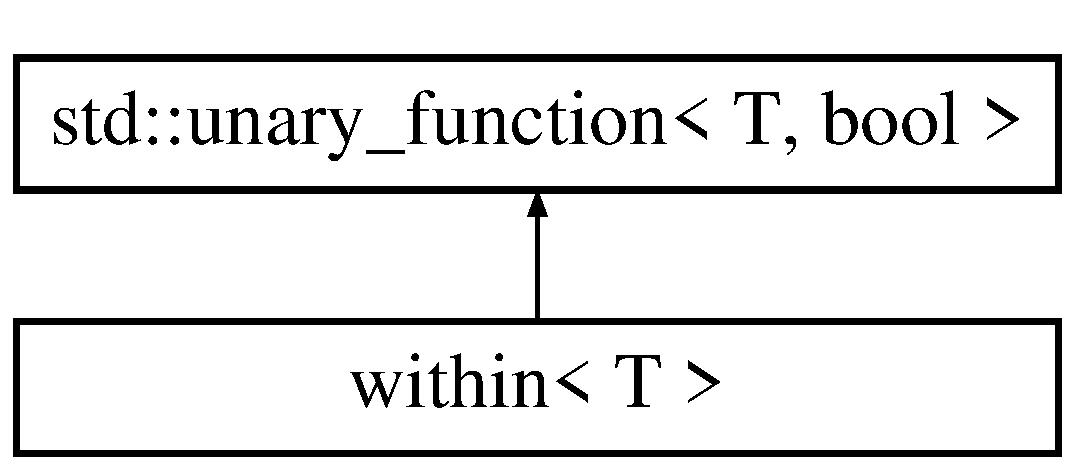
\includegraphics[height=2.000000cm]{classwithin}
\end{center}
\end{figure}
\subsection*{Public Member Functions}
\begin{DoxyCompactItemize}
\item 
{\bf within} (T range\+\_\+begin, T range\+\_\+end)
\item 
bool {\bf operator()} (T value) const 
\end{DoxyCompactItemize}


\subsection{Detailed Description}
\subsubsection*{template$<$typename T$>$\\*
class within$<$ T $>$}

Determines if a value is within a given range. 

The documentation for this class was generated from the following file\+:\begin{DoxyCompactItemize}
\item 
utilities.\+h\end{DoxyCompactItemize}

%--- End generated contents ---

% Index
\backmatter
\newpage
\phantomsection
\clearemptydoublepage
\addcontentsline{toc}{chapter}{Index}
\printindex

\end{document}
